%  library(knitr); setwd(path <- "c:/seiro/docs/external/seishin/lec_slides/2024/"); system("recycle c:/seiro/docs/external/seishin/lec_slides/2024/cache/HK"); knit("HK.rnw", "HK.tex"); system("platex HK"); system("pbibtex HK"); system("dvipdfmx HK")

\input{c:/seiro/settings/Rsetting/knitrPreamble/knitr_beamer_preamble169.rnw}
%\input{c:/seiro/settings/Rsetting/knitrPreamble/knitr_beamer_preamble169_ho.rnw}
%\input{c:/seiro/settings/Rsetting/knitrPreamble/knitr_beamer_preamble.rnw}
%\input{c:/seiro/settings/Rsetting/knitrPreamble/knitr_beamer_preamble_ho.rnw}
\definecolor{bondiaqua}{rgb}{0.0, 0.58, 0.71}
\definecolor{bondibluelight}{rgb}{0.0, 0.3, 0.41}
\definecolor{aqua}{rgb}{0.0, 1.0, 1.0}
\definecolor{bittersweet}{rgb}{1.0, 0.44, 0.37}
\definecolor{azure}{rgb}{0.0, 0.5, 1.0}
%\setbeamercolor{background canvas}{bg=bondibluelight}
\setbeamercolor{background canvas}{bg=darkdarkblue}
\setbeamercolor{normal text}{fg=white}
\setbeamercolor{item}{fg=aqua}
\mode<handout>{\setbeamercolor{item}{fg=aqua!70!black}}
\mode<handout>{\setbeamercolor{background canvas}{bg=white}}
\mode<handout>{\setbeamercolor{normal text}{fg=black}}
%\setbeameroption{show notes} %un-comment to see the notes
\hypersetup{
%linkcolor = lightblue, urlcolor = lightblue
linkcolor = blue!50, urlcolor = green!80
, citecolor = blue!50
}
\usepackage{pgfplots}
\pgfplotsset{compat=1.11} % this sets default coordinate system to axis cs in axis environment
\usetikzlibrary{intersections, arrows, calc, positioning, overlay-beamer-styles}

\setbeamercovered{invisible}
\newcommand{\DescPause}{\hspace{-.25em}\phantom{\thebeamerpauses}\pause}
\newcommand{\tikznode}[2]{%
\ifmmode%
\tikz[remember picture,baseline=(#1.base),inner sep=0pt] \node (#1) {$#2$};%
\else
\tikz[remember picture,baseline=(#1.base),inner sep=0pt] \node (#1) {#2};%
\fi}

\newcounter{angle}
\setcounter{angle}{0}
\usepackage{centernot}
\usepackage{usebib}

\begin{document}
\setlength{\baselineskip}{12pt}






\title[4]{\large 人的資本}
\author[Ito]{Seiro Ito}
\institute[IDE, Sacred Heart]{Institute of Developing Economies, Japan}
\date[Fall, 2022]{Fall, 2022\\\vspace{1ex} Department of International Exchange, Sacred Heart University}
\logo{SHU, IDE}


\frame{\titlepage}
\setcounter{page}{1}

%\setbeamercovered{transparent = 40}
%\setbeamercolor{normal text}{fg=turquoiseaqua2, bg=}
%\setbeamercolor{alerted text}{fg=black, bg=}
%\usebeamercolor{normal text}
%\setbeamercovered{transparent=0}
\def\Perp{\mkern2mu\rotatebox[origin=c]{90}{$\models$}\mkern2mu}



\begin{frame}{}
\hfil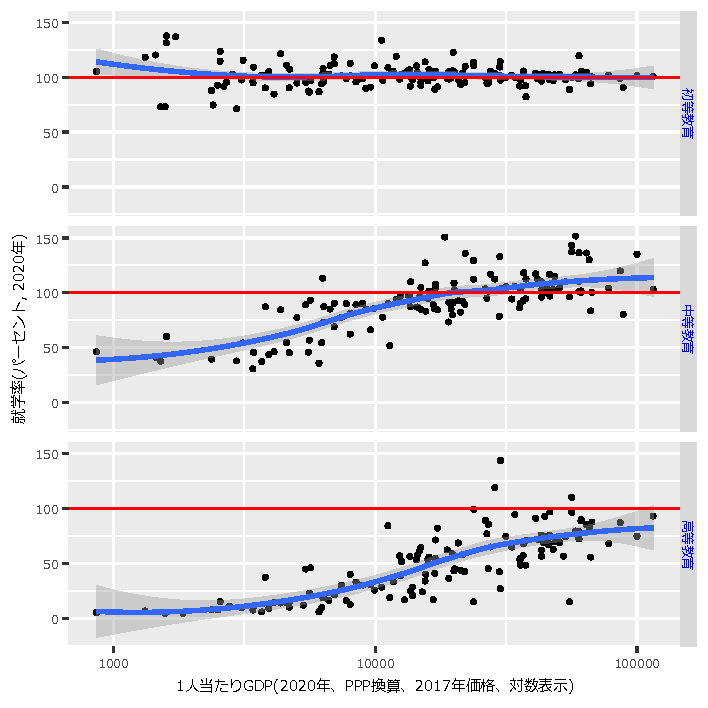
\includegraphics[height = 9cm]{c:/seiro/docs/external/seishin/lec_slides/2024/HK/figure/SG.pdf}
\end{frame}
\begin{frame}{}
\hfil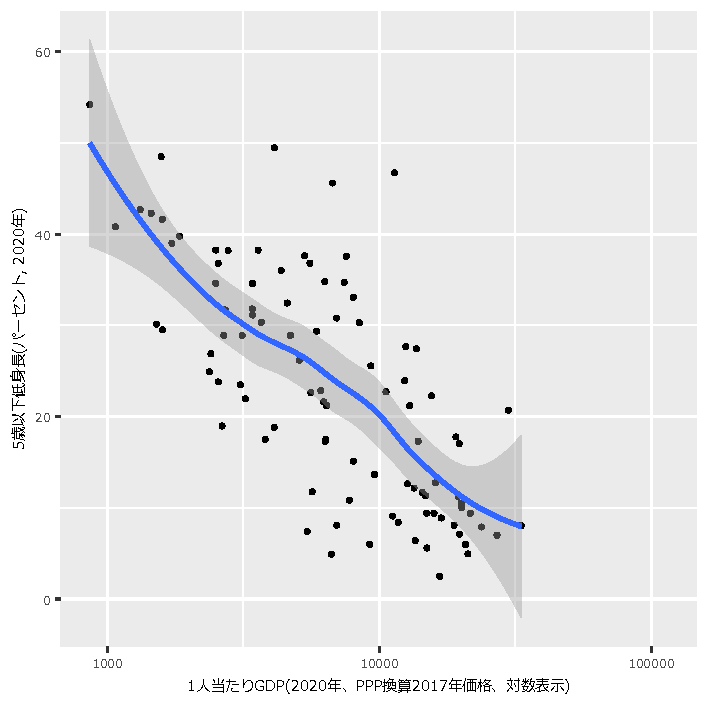
\includegraphics[height = 9cm]{c:/seiro/docs/external/seishin/lec_slides/2024/HK/figure/HG.pdf}
\end{frame}
\begin{frame}{}
\hfil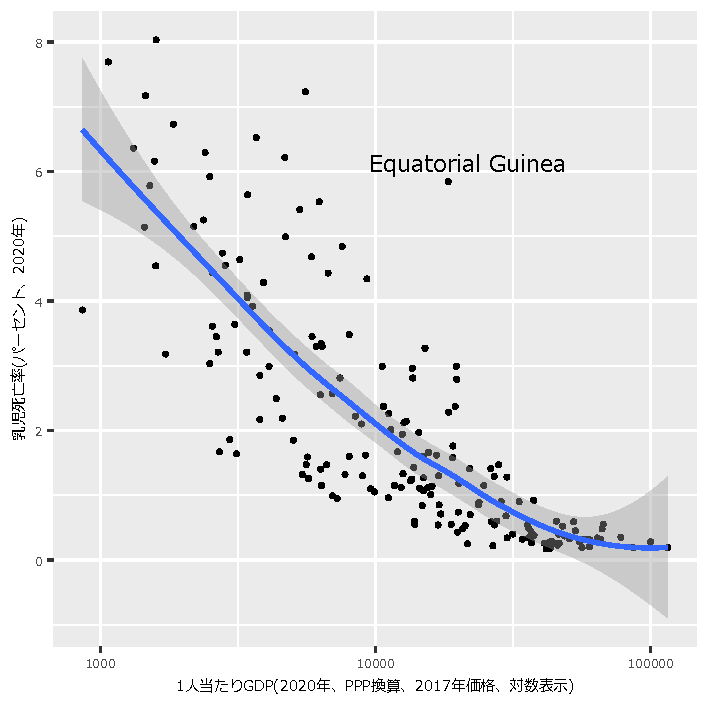
\includegraphics[height = 9cm]{c:/seiro/docs/external/seishin/lec_slides/2024/HK/figure/MG.pdf}
\end{frame}
\begin{frame}[label=WhatIsHumanCapital]{}
人的資本とは\\~\\
\pause
教育、訓練、健康(保健)など、人間の生産性を高める無形資産。\\~\\
\pause
古くはアダム・スミスにその概念が見出されるが、近代になって提唱したのがアメリカの経済発展を研究した\citet{Schultz1960, Schultz1961}、賃金を職歴と教育水準に関連づける実証研究をした\citet{Mincer1974}、最適な人的資本投資に関する理論的貢献をした\citet{Becker1962, Becker1964}など。\\~\\
\pause
教育水準や保健指標が優れているほど所得は高いので、教育や保健の普及が所得を増やすかもしれない...\\~\\
\pause
貧困の罠では経済全体が豊かになるメカニズムとその障壁を考えた\\~\\
このセクションでは、個々の家計が豊かになるメカニズムを人的資本投資を通じて考える
\end{frame}









\begin{frame}{}
\begin{columns}[T]
\column{.75\textwidth}
\onslide<1->{被雇用者1人あたりGDP(労働生産性)\\
\vspace{-0ex}
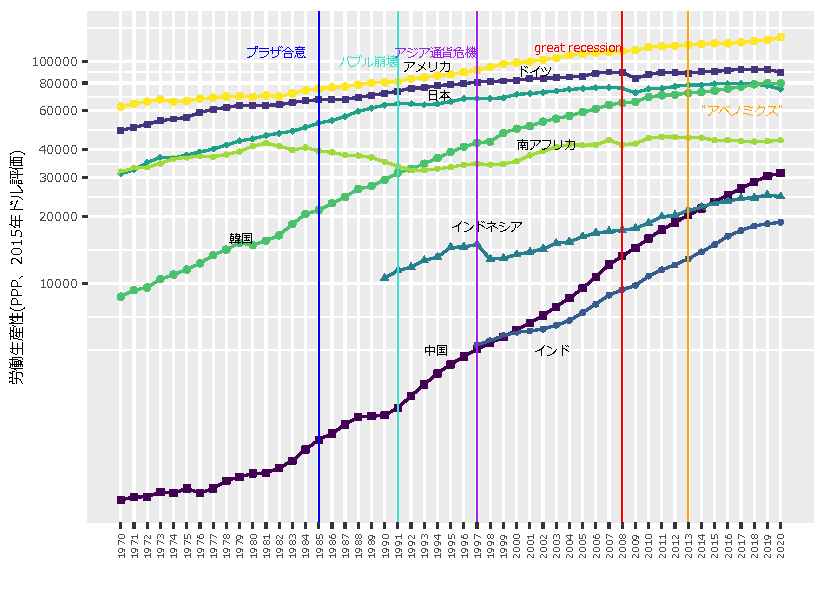
\includegraphics[height = 7.25cm, width = 12cm]{c:/seiro/docs/external/seishin/lec_slides/2024/HK/figure/LabourProductivityPerEmployee.pdf}\\
{\scriptsize 出所: \href{https://stats.oecd.org/Index.aspx?DataSetCode=PDB_LV}{OECD}}
}
\column{.25\textwidth}
\begin{itemize}\footnotesize
\vspace{1.0ex}\setlength{\itemsep}{1.0ex}\setlength{\baselineskip}{9pt}
\onslide<2->{\item	中国、韓国、インドの労働生産性は急速に成長、ただし、インドの水準はまだ低い}
\onslide<3->{\item	南アフリカとインドネシアの労働生産性は低く、成長も遅い}
%\onslide<4->{\item	インドネシア、韓国、アメリカはリーマン後の成長が似ている}
\onslide<4->{\item	リーマン・ショックを引き起こしたアメリカは、ショック後も労働生産性が成長}
\end{itemize}
\end{columns}
\end{frame}

\begin{frame}{}
\begin{columns}[T]
\column{.75\textwidth}
\onslide<1->{被雇用者1人あたりGDP(労働生産性): 現在の高所得国のみ\\
\vspace{-0ex}
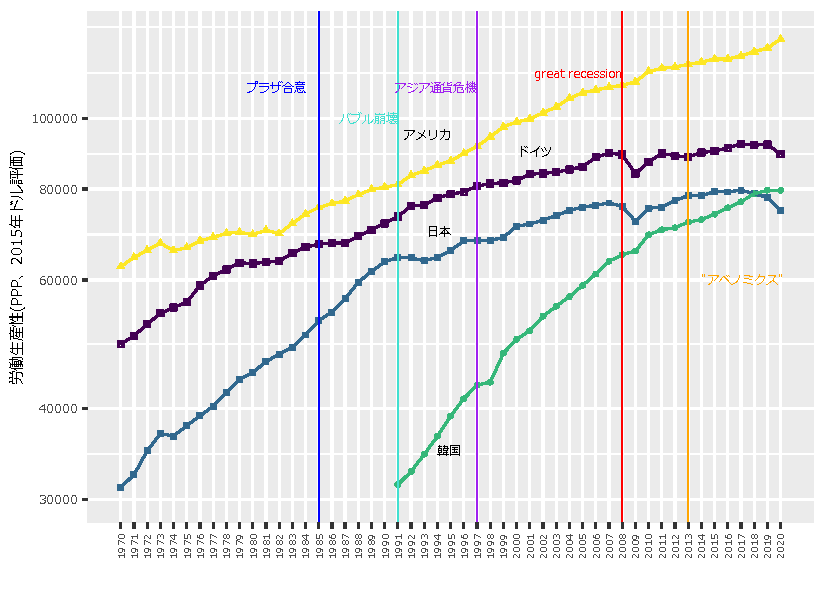
\includegraphics[height = 7.25cm, width = 12cm]{c:/seiro/docs/external/seishin/lec_slides/2024/HK/figure/LabourProductivityPerEmployee2.pdf}\\
{\scriptsize 出所: \href{https://stats.oecd.org/Index.aspx?DataSetCode=PDB_LV}{OECD}}
}
\column{.25\textwidth}
\begin{itemize}\footnotesize
\vspace{1.0ex}\setlength{\itemsep}{1.0ex}\setlength{\baselineskip}{9pt}
\onslide<2->{\item	日本の労働生産性はバブル崩壊後も1996年頃までアメリカと似た成長率、それ以降は差が拡大}
\onslide<3->{\item	1990年代末期は就職氷河期、デフレの始まり(CPI, 1998年9月)}
\onslide<4->{\item	2011年大震災以降、労働生産性は僅かに上昇したが、アベノミクス以降も成長せず、COVID-19蔓延以前の2018年から低下}
\end{itemize}
\end{columns}
\end{frame}

\begin{frame}{}
\begin{columns}[T]
\column{.75\textwidth}
\onslide<1->{1人あたりGDP\\
\vspace{-0ex}
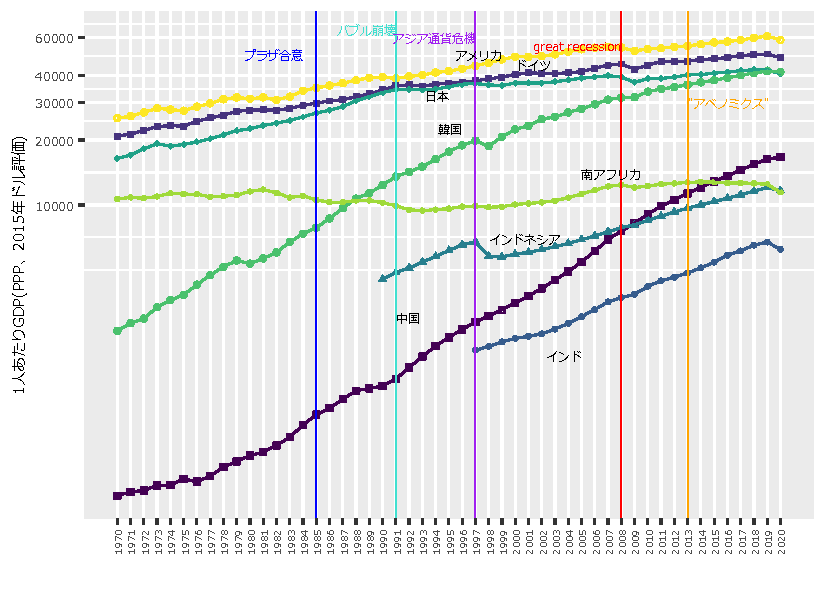
\includegraphics[height = 7.25cm, width = 12cm]{c:/seiro/docs/external/seishin/lec_slides/2024/HK/figure/GDPPerCapita.pdf}\\
{\scriptsize 出所: \href{https://stats.oecd.org/Index.aspx?DataSetCode=PDB_LV}{OECD}
}
}
\column{.25\textwidth}
\begin{itemize}\footnotesize
\vspace{1.0ex}\setlength{\itemsep}{1.0ex}\setlength{\baselineskip}{9pt}
\onslide<2->{\item	1人当たりGDPは労働生産性とトレンドと近似}
\onslide<3->{\item	低所得国と高所得国の差は縮まっている}
\onslide<4->{\item	南アフリカはインドネシアに追いつかれた}
\onslide<5->{\item	1人当たりGDPでも日本は韓国に追いつかれた}
\onslide<6->{\item	南アフリカは中国よりも労働生産性は高いが1人当たりGDPは低い}
\end{itemize}
\end{columns}
\end{frame}

\begin{frame}{}
\begin{columns}[T]
\column{.75\textwidth}
\onslide<1->{1人あたりGDP: 現在の高所得国のみ\\
\vspace{-0ex}
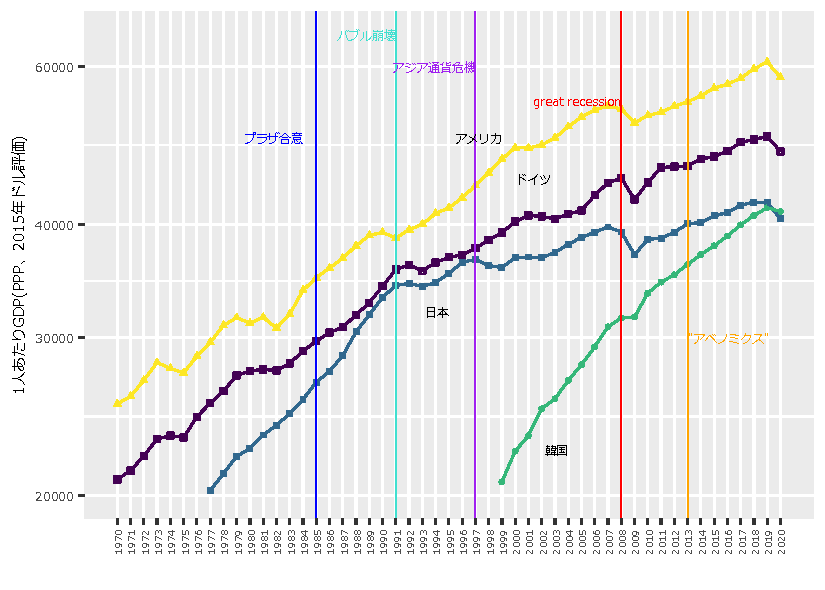
\includegraphics[height = 7.25cm, width = 12cm]{c:/seiro/docs/external/seishin/lec_slides/2024/HK/figure/GDPPerCapita2.pdf}\\
{\scriptsize 出所: \href{https://stats.oecd.org/Index.aspx?DataSetCode=PDB_LV}{OECD}
}
}
\column{.25\textwidth}
\begin{itemize}\footnotesize
\vspace{1.0ex}\setlength{\itemsep}{1.0ex}\setlength{\baselineskip}{9pt}
\onslide<2->{\item	日本は1997年からアメリカとドイツとの格差拡大}
\onslide<3->{\item	日本はアベノミクスの1年前から成長}
\onslide<4->{\item	日本は労働生産性は低迷しているのに1人当たりGDPは成長}
\end{itemize}
\begin{dinglist}{45}
\vspace{1.0ex}\setlength{\itemsep}{1.0ex}\setlength{\baselineskip}{12pt}
\onslide<5->{\item	就労人数(時間人)が増えたため?}
\end{dinglist}
\end{columns}
\end{frame}





\begin{frame}[label=KShare]{}
資本分配率(=資本報酬/国民所得=1-労働分配率)\\
\vspace{-0ex}
\hfil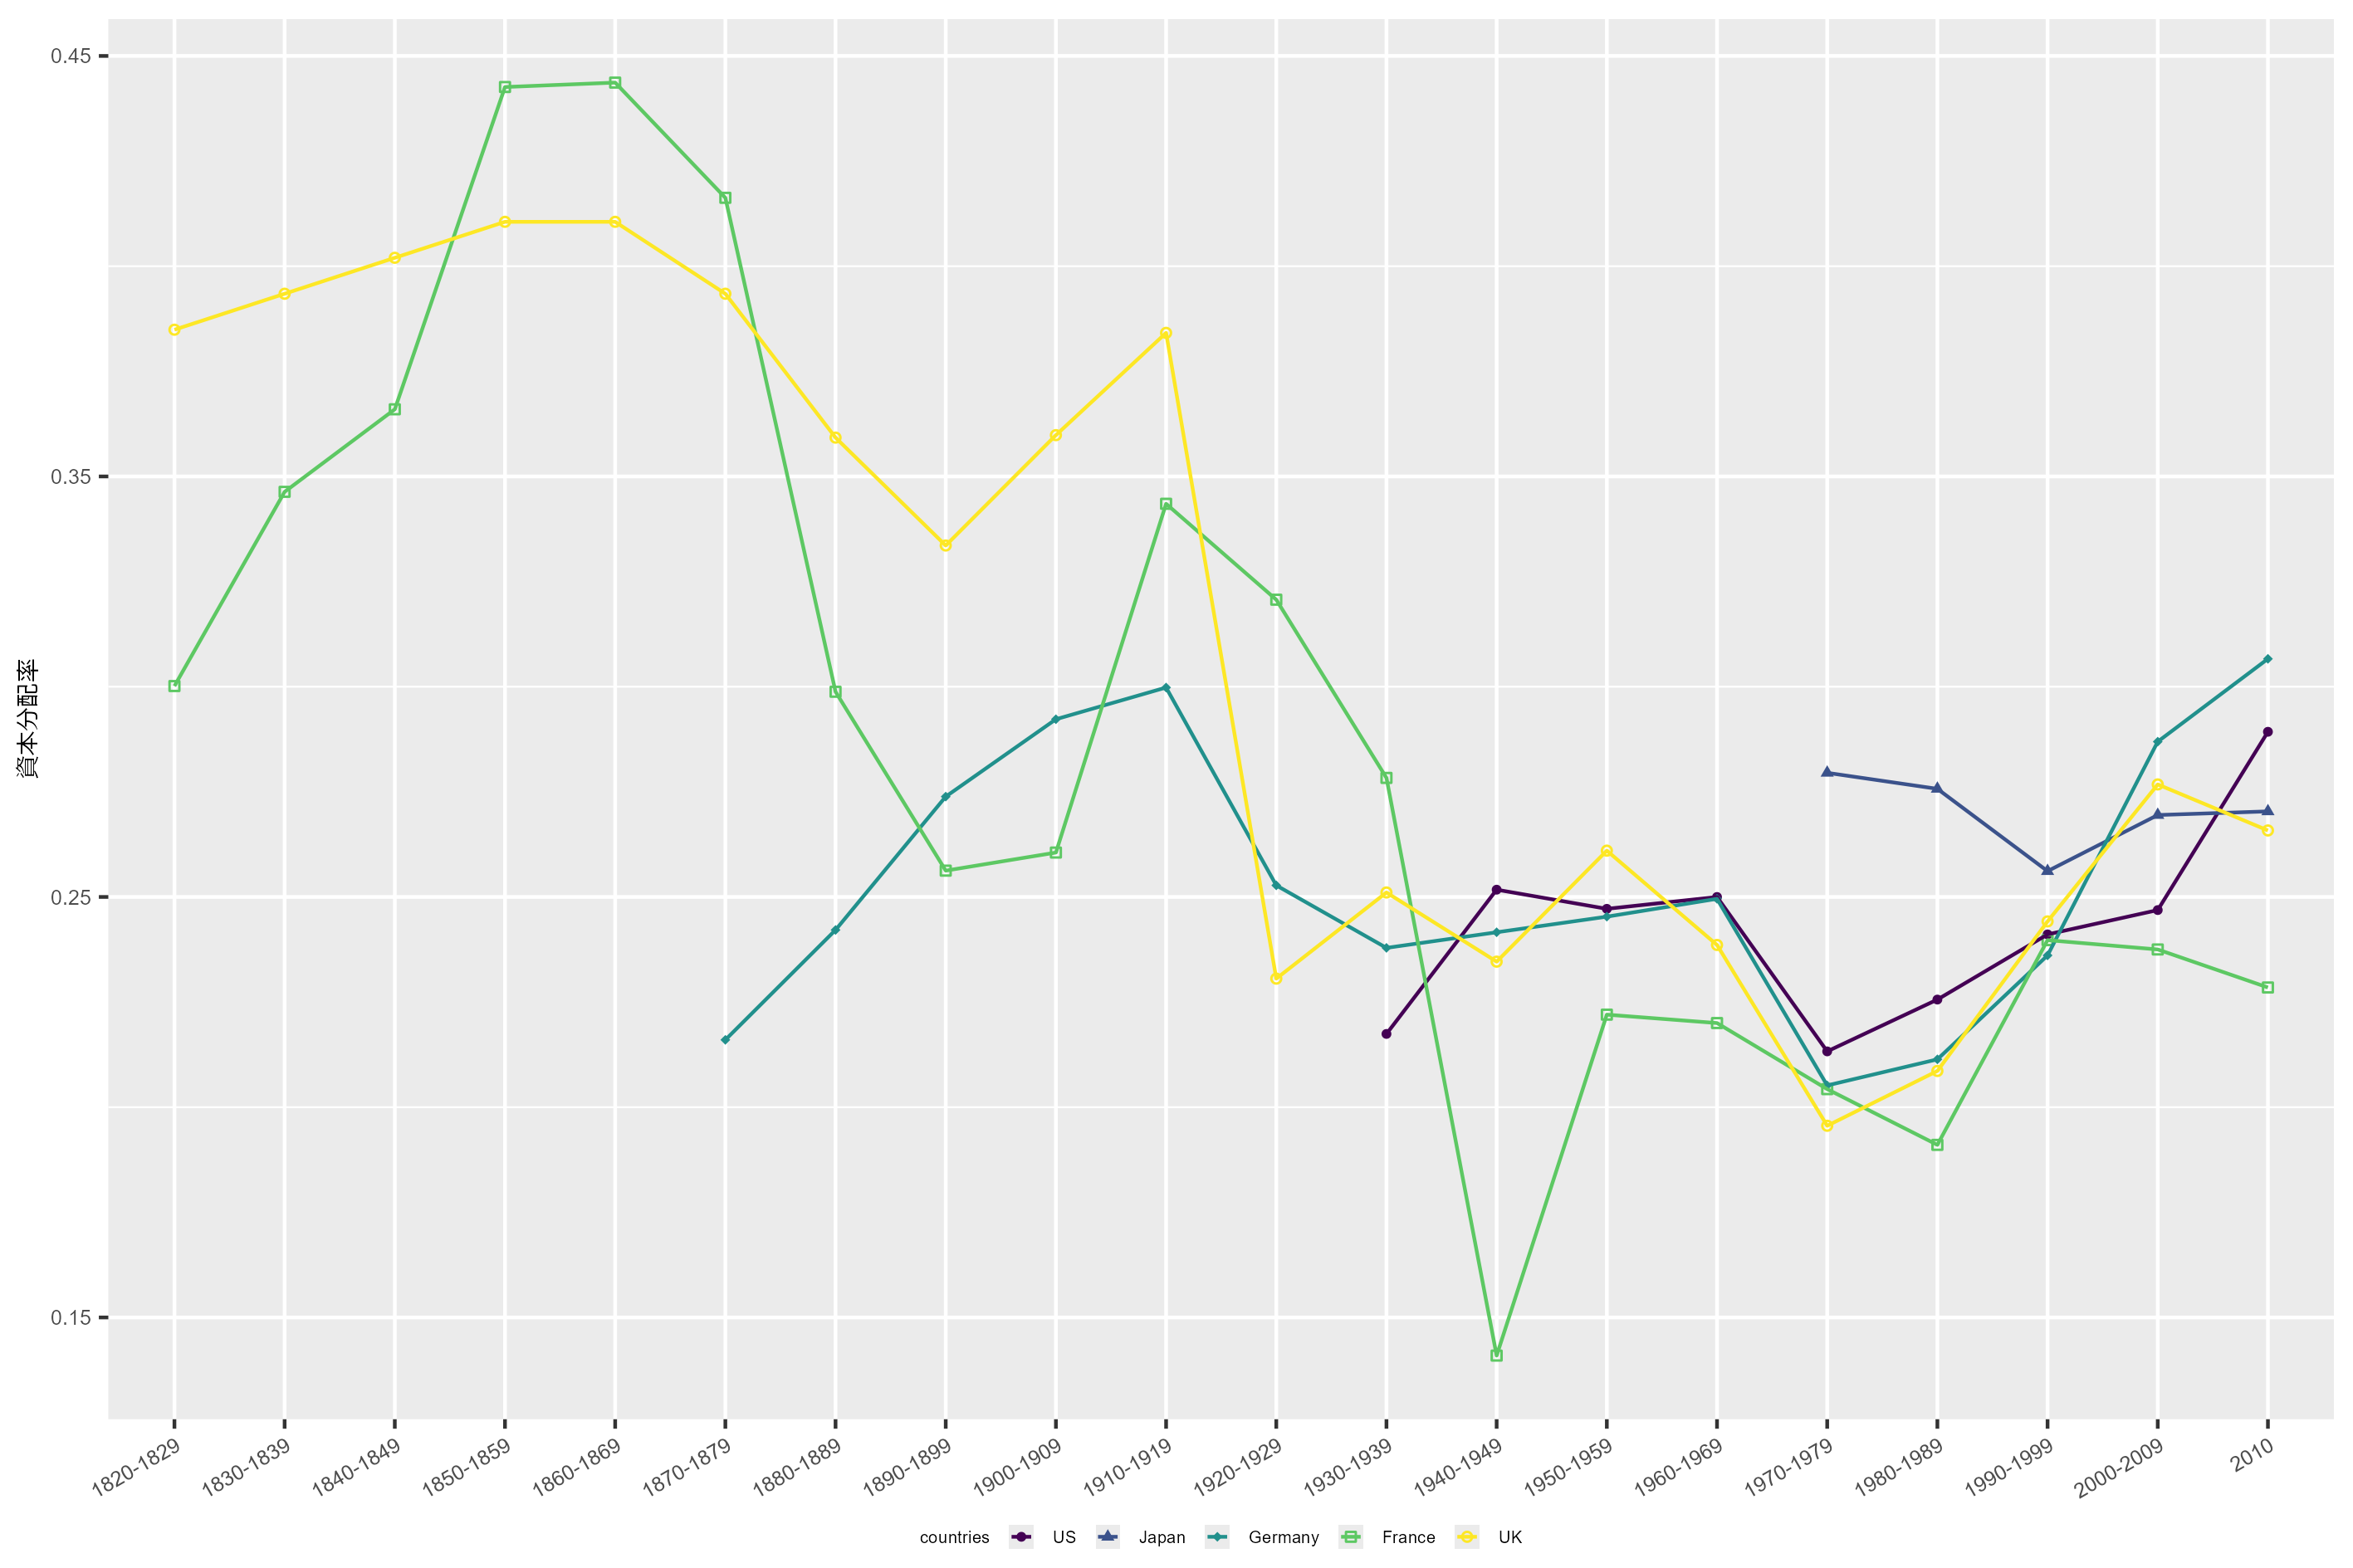
\includegraphics[height = 7cm, width = 12cm]{c:/seiro/docs/external/seishin/lec_slides/2024/HK/figure/PikettySaezZucman.png}\\
{\footnotesize 出所: \citet[][Table A49]{PikettySaezZucman2018}より作成。}
\end{frame}


\begin{frame}[label=Schultz]{}
\citet{Schultz1960}の疑問と仮説\\~\\
\pause
労働人口や資本の増加以上に生産が増えているのはなぜか
\pause
\begin{dinglist}{43}
\vspace{1.0ex}\setlength{\itemsep}{1.0ex}\setlength{\baselineskip}{12pt}
\item	つまり、生産額/労働量=労働生産性、生産額/資本サービス価値=資本生産性が増えているのはなぜか
	\begin{dinglist}{45}
	\vspace{1.0ex}\setlength{\itemsep}{1.0ex}\setlength{\baselineskip}{12pt}
	\item	国内総生産(GDP)/人口=1人当たりGDP(労働人口$<$人口だが国単位での労働生産性を近似)も増えている。
	\end{dinglist}
\end{dinglist}
\pause
\vspace{2ex}
労働分配率はなぜ上昇しているのか(1960年当時)\hfill\hyperlink{LShare<1>}{\beamergotobutton{先進国労働分配率}}
\\~\\
\pause
人間への投資が労働生産性を高めているため\\~\\
\pause
人間への投資の成果=人的資本human capital\\~\\
\pause
人間を資本という物として捉えるのは当時(現在も?)「けしからん」\\~\\
\pause
\citet{Becker1964}も\textit{Human Capital: A theoretical and empirical analysis, with special reference to education}などと副題を付けた
\end{frame}

\begin{frame}[label=DefineHumanK]{}
人的資本の分類
\begin{description}
\vspace{1.0ex}\setlength{\itemsep}{1.0ex}\setlength{\baselineskip}{12pt}
\pause
\item[知的能力]	知識、技能
\pause
\item[物的能力]	健康
\end{description}
\vspace{1ex}
\begin{dinglist}{43}
\vspace{1.0ex}\setlength{\itemsep}{1.0ex}\setlength{\baselineskip}{12pt}
\pause
\item	知識と技能は性質が異なる
	\begin{itemize}
	\vspace{1.0ex}\setlength{\itemsep}{1.0ex}\setlength{\baselineskip}{12pt}
	\pause
	\item	技能: 人間に体化される\pause 私的財
	\pause
	\item	知識: 社会に蓄積されて共有される. \pause 公共財: 他者の消費は競合しないし排除もできない
	\end{itemize}
\pause
\item	健康は運動能力と感染源(!)に分けると性質が異なる
	\begin{itemize}
	\vspace{1.0ex}\setlength{\itemsep}{1.0ex}\setlength{\baselineskip}{12pt}
	\pause
	\item	運動能力: 人間に体化される\pause 私的財
	\pause
	\item	感染源: 社会に広める. \pause 外部性のある私的財: 他者への影響が市場で価格評価されないので、個人の行動は他者への感染を考慮しにくい
	\note[item]<11>{自分は軽症にしかならないから、感染予防努力を緩める}
   \note[item]<11>{マスク着用を強要するのは自由の侵害だ、自由のためなら自分は感染する覚悟がある}
		\begin{dinglist}{45}
		\vspace{1.0ex}\setlength{\itemsep}{1.0ex}\setlength{\baselineskip}{12pt}
		\item	予防努力 %自分は軽症にしかならないから、感染予防努力を緩める
		\item	自由の侵害 %マスク着用を強要するのは自由の侵害だ、自由のためなら自分は感染する覚悟がある
		\end{dinglist}
	\end{itemize}
\end{dinglist}
\end{frame}

\begin{frame}[label=KnowledgeProduction]{}
知識生産=研究開発(R\&D)活動。\\~\\
\pause
模倣されると利益が減るので、知識生産は社会的に最適水準よりも少なくなりがち。\\~\\
\pause
特許patents、著作権copyright、商標trademarkなどで知的財産権を保護して少なくなりすぎないようにする。\\~\\
\pause
原則は理解されても、保護や違反摘発・懲罰の適切な水準に合意がない。
\end{frame}

\begin{frame}[label=PatentExamples]{}
\begin{itemize}
\vspace{1.0ex}\setlength{\itemsep}{1.0ex}\setlength{\baselineskip}{12pt}
\pause
\item	キムリア(白血病やリンパ腫、1回投与で3349万円)、ザインテグロ(ベータ・サラセミア、米承認3億円)
\pause
\item	保護下で薬価を高くし過ぎたために利用が進まない: Truvada(HIV予防治療薬)
\pause
\item	低所得者対象で利益が少ない+模倣されやすいために開発が進まない: マラリア治療薬、結核治療薬などのneglected tropical diseases
\pause
\item	厳しい罰則(日本: 商標権を侵害した場合は10年以下の懲役もしくは1000万円以下の罰金)、でも、生産地中国での摘発は...: 偽ブランド品販売
\pause
\item	著作権の保護期間を再三延ばすことで多額の利潤を保有権者が得る: ミッキーマウス(1923年生まれ、1998年期限切れ予定、1998年期限延長、2024年期限切れ予定[US])
	\begin{dinglist}{45}\footnotesize
	\vspace{1.0ex}\setlength{\itemsep}{1.0ex}\setlength{\baselineskip}{12pt}
	\pause
	\item	 \href{https://arstechnica.com/tech-policy/2019/01/a-whole-years-worth-of-works-just-fell-into-the-public-domain/}{(I)t was ``basically the Gershwin family trust, grandchildren of Oscar Hammerstein, Disney, others of that ilk'' who pushed for ever-longer copyright terms.} (Dennis Karjala, Law professor, 2013)
	\pause
	\item	商標はディズニーが半永久的に保有し続ける。ミッキーマウスの絵はpublic domainになるが、ミッキーの何々、という使い方は商標の使用許諾を得た上でライセンス料を支払う。
	\end{dinglist}
\end{itemize}
\end{frame}

\begin{frame}[label=IntellectualProperty]{Intellectual capacity}
人の中で知的能力はどのように成長するでしょうか。
%How does intellectual capacity grow in a person?
\\~\\
\pause
学校教育を考えます。%Let us consider schooling.
\\~\\
\pause
通学すると学習し、人的資本(知的能力)を蓄積し、生産性が高まります。%If you go to a school, you learn, you will accummulate human capital (intellectual capacity), and you will become productive.
\\~\\
\pause
生産性が高いほど稼ぎが増えます。%The more you are productive, the more you earn.
\\~\\
\pause
では、できる限り長く学校に通うべきでしょうか? %Then, shall we go to school as long as possible?
\pause
いいえ、ある段階で止めて働かねばなりません。%No. You need to stop at some point and start to work.
\\~\\
\pause
いつ止めるかどのように決めるべきでしょうか。%How do we decide when to stop?
\\~\\
\pause
止めるタイミングを理解するには理論が必要になります。%We need a theory to understand.
\end{frame}

\begin{frame}[label=BalandRobinson]{}
\citet{BalandRobinson2000}モデル: 2期間モデルを考えます。
Here comes \citet{BalandRobinson2000}: Let us consider a two-period model.

\begin{description}
\vspace{1.0ex}\setlength{\itemsep}{1.0ex}\setlength{\baselineskip}{12pt}
\pause
\item[第1期]	子ども期: どのくらい学校に行くか、どのくらい働くか決めます。You choose how much to go to school, how much to work.
\pause
\item[第2期]	成人期: 労働所得を得ます。成人期所得は子ども期の就学期間に応じて増えます。You earn. Adulthood income is increasing in childhood schooling.
\end{description}
\end{frame}

\begin{frame}{}
合理的な子ども: 便益と費用を考慮して教育水準を決める
\begin{description}
\vspace{1.0ex}\setlength{\itemsep}{1.0ex}\setlength{\baselineskip}{12pt}
\pause
\item[便益]	学歴を積むことによる成人所得増加分$\times$割引率
\pause
\item[費用]	学歴を積むことによる就学費用(=学費+制服・給食・通学その他費+児童労働所得)
\end{description}
\vspace{2ex}
\pause
教育水準を決める=第1期の時間配分(就学 vs. 就労)を決める\\~\\
\pause
単純化のため学費+制服・給食・通学その他費=0と仮定する
\pause
\begin{dinglist}{43}
\vspace{1.0ex}\setlength{\itemsep}{1.0ex}\setlength{\baselineskip}{12pt}
\item	以下の場合、親は子どもが判断するよりも児童労働就労時間を長くして、子どもの児童労働所得で自分の効用を高める
	\begin{itemize}
	\vspace{1.0ex}\setlength{\itemsep}{1.0ex}\setlength{\baselineskip}{12pt}
\pause
	\item	親が子どもの成人期所得効用を子どもが感じるよりも割り引くとき(将来よりも現在の家族の幸せ)
\pause
	\item	「成人したら仕送りを約束するから学校に行かせてほしい」と子どもが頼んでも、親が子どもの約束を信じないとき(子どもは将来裏切ることができるため)
	\end{itemize}
\pause
\item	意志決定者が子どもか親かによって人的資本投資額が変わる
\end{dinglist}
\end{frame}

\begin{frame}{}
教育の人的資本仮説: 学歴水準の決定=生産性向上手段
\begin{dinglist}{45}
\vspace{1.0ex}\setlength{\itemsep}{1.0ex}\setlength{\baselineskip}{12pt}
\pause
\item	人的資本仮説と補完的な見方: 
	\begin{description}
	\vspace{1.0ex}\setlength{\itemsep}{1.0ex}\setlength{\baselineskip}{12pt}
	\item[シグナリング仮説]	学歴水準の決定=(雇用者への)能力情報伝達手段(あくまでもシグナルであって、生産性を変えても変えなくてもいい)
	\end{description}
\pause
\item	シグナリング・モデルでは、就学や学習の費用が低い人ほど教育水準を高く選ぶ
\end{dinglist}
\vspace{2ex}
\pause
人生効用最大化のために子どもは何を決めるか\\~\\
\pause
第1期時間配分、第1期と第2期の間の消費配分\\~\\
\pause
理解の段取り: 
\begin{enumerate}
\vspace{1.0ex}\setlength{\itemsep}{1.0ex}\setlength{\baselineskip}{12pt}
\pause
\item	第1期時間配分を最適に決め、人生を通じて所得合計を最大化する
\pause
\item	各期への消費配分を決める
\end{enumerate}
\end{frame}


\begin{frame}{}
ミクロ経済学: 限界収入=限界費用(MR = MC)\\~\\

\pause
生涯効用を最大化する最適な学歴水準$l^{*}$(第1期の時間配分)は下記を満たすはず
\[
\underbrace{\mbox{\small 成人所得増加による効用増加分}}_{\mbox{\footnotesize 就学の限界収入(を効用評価)}} = \underbrace{\mbox{\small 児童労働所得減少による効用減少分}}_{\mbox{\footnotesize 就学の限界費用(を効用評価)}}
\]

\vspace{2ex}
\pause
第1期の時間配分は現時点での(限界)費用と将来時点の(限界)便益をバランスさせるように決まる\\[.5ex]

\begin{columns}[T]
\column{.4\textwidth}
\hfil\begin{tikzpicture}[ 
axis/.style={very thick, ->, >=stealth'},
dashed line/.style={dashed, thin},
every node/.style={},
background rectangle/.style = {fill = gray90},
]
\begin{axis}[
  scale = .7,
  axis equal image, % forces a square plot
  clip = false, % allows plotting outside axis bounds
  axis x line=center, axis y line=center,
  xlabel = {$l$}, ylabel = {$MC, MR$},
  xtick={100}, ytick={100}, % effectively drops axis ticks
  xlabel style={below right}, ylabel style={above left},
  xmin=0, xmax=11,
  ymin=0, ymax=10]
\coordinate (origin) at (axis cs: 0, 0) ;
\path[name path=xaxis, gray] (0, 0) -- (axis cs: 10, 0);
\path[name path=yaxis, gray] (0, 0) -- (axis cs: 0, 10);
% curves
\addplot [name path=MBcurve, no marks, line width = .5pt, domain=0.01:7, smooth] {8-.8*x} node[below right] (MBend) {\small $MR(l)$};
\addplot [name path=MCcurve, no marks, line width = .5pt, domain=0.01:7, smooth] {1+.8*x} node[above right] (MCend) {\small $MC(l)$};
% intersection, x and y coordinates of intersections
\path [name intersections={of=MBcurve and MCcurve, by={e1}}];
\coordinate (e1Xaxis) at (e1 |- origin) ;
\coordinate (e1Yaxis) at (e1 -| origin);
\draw [name path=Hor1, azure, line width = .5pt, dashed] (e1) -- (e1Yaxis) node[left] {\small $MR=MC$};
\draw [name path=Ver1, azure, line width = .5pt, dashed] (e1)  -- (e1Xaxis) node[below] {\small $l^{*}$};
% intersections of curves
\fill [azure] (e1) circle (3pt);
\draw (axis cs: 0, 8) node[left] {};
\draw (axis cs: 0, 1) node[left] {};
\end{axis}
\end{tikzpicture}
\column{.6\textwidth}
\pause
MR$>$MCのとき=$l<l^{*}$のとき、$l$を僅かに増やせば$MR-MC$だけ純利益を増やせる$\rightarrow l$を増やす\\[1ex]
\pause
$\because$不等号ならば、$l$を増減することで限界的な純利益を拡大できるから。等号ならば、改善の余地がないということ。\\[1ex]
\pause
連続関数の最大化: 限界収入=限界費用(MR-MC=0)、を図解できる (スライド: 微分)
\end{columns}
\end{frame}

\begin{frame}{}
$t$期の消費$c_{t}$よる効用$u(c_{t})$, $t=1,2$\\~\\
\pause
初期資産$A$、貯蓄$s$、就学時間$l$、児童労働賃金$w$\\~\\
\hfil\begin{tabular}{
>{\hfill}p{3cm}<{}
>{$}p{6cm}<{$\hfill}
}
就労時間 & 24-l\\
児童労働所得 & w\times(24-l)\\
児童時消費 & w\times(24-l)+A-s\\
児童時効用 & u\{w(24-l)+A-s\}=u(c_{1})\\
\pause
成人所得 & h(l)\\
成人時効用 & u\{Rs+h(l)\}=u(c_{2})\\
\end{tabular}

\begin{itemize}
\vspace{1.0ex}\setlength{\itemsep}{1.0ex}\setlength{\baselineskip}{12pt}
%\item	児童労働所得は(24時間から就学時間$l$を引いた)就労時間*児童労働賃金。成人所得は就学時間の増加関数。
%\item	児童労働時間は児童労働所得を増やして成人所得を減らす$=$就学時間は児童労働所得を減らして成人所得を増やす
\item	児童労働時間の決定には今期所得と将来所得のトレードオフがある
	\begin{dinglist}{45}
	\vspace{1.0ex}\setlength{\itemsep}{1.0ex}\setlength{\baselineskip}{12pt}
	\item	トレードオフをどのように選ぶかを考えるのが経済学
	\end{dinglist}
\end{itemize}
\end{frame}

\begin{frame}{}
生涯効用最大化問題として今期所得と来期所得のトレードオフを考える\\~\\
生涯効用最大化問題として児童労働時間=$24-$就学時間=$24-$人的資本投資時間を考える
\[
\begin{aligned}
\max_{\{s, l\}}
\;\;\; & u(c_{1})+\beta u(c_{2}) \hspace{1cm} &&\mbox{\textcolor{aqua}{\mpage{4cm}{\scriptsize $s,l$を操作して生涯効用\hfill\\ $u(c_{1})+\beta u(c_{2})$を最大化\hfill}}}\\
\st \;\;\; 
& c_{1}=w(24-l)+A-s  &&\mbox{\textcolor{aqua}{\mpage{4cm}{\scriptsize $c_{1}$は児童労働所得+資産-貯蓄\hfill}}}\\
& c_{2}=h(l)+Rs  &&\mbox{\textcolor{aqua}{\mpage{4cm}{\scriptsize $c_{2}$は成人所得+R*貯蓄\hfill}}}
\end{aligned}
\]
2つの制約を目的関数に代入すると、制約条件を組み込んだ目的関数になる
\[
\max_{\{s, l\}}
\;\;\; u\left\{w(24-l)+A-s\right\}+\beta u\left\{h(l)+Rs\right\}
\]
\end{frame}

\begin{frame}{}
最大化するには変動させる変数で微分してゼロとおく(「最大化の一階条件」first order conditions for the maximumといいます)
\[
\begin{aligned}
u_{s}
&=-u'\left\{w(24-l)+A-s\right\}+\beta Ru'\left\{h(l)+Rs\right\}=0,\\
u_{l}
&=-wu'\left\{w(24-l)+A-s\right\}+\beta h'(l)u'\left\{h(l)+Rs\right\}=0.
\end{aligned}
\]
$u_{l}=0$を変形すると
\[
\underbrace{wu'\left\{w(24-l)+A-s\right\}}_{\mbox{\mpage{6cm}{\footnotesize 就学による児童労働所得減の効用減少分\\\hfil 就学の限界費用(を効用評価)}}}= \underbrace{\beta u'\left\{h(l)+Rs\right\}h'(l)}_{\mbox{\mpage{6cm}{\footnotesize 就学による成人所得増の効用増加分\\\hfil 就学の限界収入(を効用評価)}}}
\]
\pause
就学時間増による成人所得増加の効用増加分=成人所得増加分$\times$成人時効用増加$=h'(l)u'\{h(l)+Rs\}$\\~\\
\pause
就学時間増による児童労働所得減少の効用減少分=児童所得減少分$\times$児童時効用減少=児童労働賃金$\times$児童時効用減少$=w\times -u'\{w(24-l)+A-s\}=-u'\{w(24-l)+A-s\}w$\\~\\

\end{frame}

\begin{frame}{}
経済学でよく使われる仮定
\begin{description}
\vspace{1.0ex}\setlength{\itemsep}{1.0ex}\setlength{\baselineskip}{12pt}
\item[限界生産力逓減の仮定]	技術が変わらずに生産要素が増えると、生産の増加幅は低下するという仮定
	\begin{dinglist}{45}
	\vspace{1.0ex}\setlength{\itemsep}{1.0ex}\setlength{\baselineskip}{12pt}
\pause 
	\item	$h(l)$: 就学$l$のときの成人所得
	\item	$h'(l)$: 就学$l$で$l$を増やしたときの成人所得変化 \quad \textcolor{aqua}{$l$での$h(l)$の傾き}
	\item	$h'(l)$は$l\in\mathbb R_{+}$で非負 \quad \textcolor{aqua}{$R_{+}$=正の実数すべての集合}
	\item	$h'(l)$は$l$とともに減少、$h''(l)<0$ \quad \textcolor{aqua}{$l$での$h(l)$の傾きは減っていく}
	\end{dinglist}
\pause
\item[限界効用逓減の仮定]	消費水準が増えると、効用の増加幅は低下するという仮定
	\begin{dinglist}{45}
	\vspace{1.0ex}\setlength{\itemsep}{1.0ex}\setlength{\baselineskip}{12pt}
\pause 
	\item	$u'(c)$は$c\in\mathbb R_{+}$で非負
	\item	$u'(c_{t})$は$c_{t}$とともに減少、$u''(c_{t})<0$
	\end{dinglist}
\end{description}
\end{frame}

\begin{frame}{}
\[
wu'\left\{w(24-l)+A-s\right\}=\beta u'\left\{h(l)+Rs\right\}h'(l).
\]

\vspace{3ex}
$wu'\left\{w(24-l)+A-s\right\}$は$l$が大きいほど$\left\{\cdot\right\}$括弧の中が小さい $\Rightarrow$ $u'\left\{\cdot\right\}$が大きい ($\because$限界効用逓減) $\Rightarrow$ \textcolor{darkred}{左辺$u'\left\{\cdot\right\}$は$l$の増加関数}\\~\\
$u'\left\{h(l)+Rs\right\}h'(l)$は$l$が大きいほど$u'\left\{h(l)+Rs\right\}$も$h'(l)$も小さくなる ($\because$限界効用逓減、限界生産力逓減) $\Rightarrow$ \textcolor{green!80}{右辺$u'\left\{h(l)+Rs\right\}h'(l)$は$l$の減少関数}\\~\\
\end{frame}


\def\xlow{3.83}
\def\xadd{1.87}
\def\xpivot{3.2}
\def\xpivothalf{1.6}
\def\xpivothalftwo{5.6}
\def\xright2{4}
\def\Xlim{12}
\def\Ylim{8}
\def\Ylimtwo{12}
\def\yminus{-.25}

%\def\xpivothalf{\divide \xpivot by 2}
%\def\divider{2}
%\def\xpivothalf{\xpivot / \divider}
\def\ProdFunction{(0, 7) to [out=-10, in=170] (6.5, \xright2) }
\def\afterline{(0, 4) to [out=20, in=190] (\Xlim-1, 7)}
\tikzstyle{line} = [draw, very thick, -latex']

%\setbeamercovered{transparent=20}
\begin{frame}[b]{児童の時間配分決定}
%\def\ProdFunction{(0, 3) parabola bend (5,4) (8, 4.44)}
\hfil\begin{tikzpicture}[scale=.75]
% use only, not onslide, otherwise onslide produces blank spots at all intersections
\onslide<1->{
	\coordinate(origin) at (0, 0);
	\coordinate(TopLeft) at (0, \Ylim);
	\coordinate(BottomRight) at (\Xlim, 0);
	\coordinate(XRight) at (\Xlim-1, 0);
	\coordinate(TopRight) at (\Xlim-1, \Ylim);
	\draw (origin) -- (\Xlim, 0) node[right] {就学時間$l$};
	\draw[->, line, name path = YAxis] (origin) -- (0, \Ylim) node[above] {限界効用};
}
\onslide<2->{
	\draw (XRight) -- (TopRight) node[above] {24};
}
\only<3->{
	\draw[name path=MPcurve, draw, color=green!80, thick] 
	  \ProdFunction node[right] {\mpage{3cm}{\footnotesize 就学便益の限界効用\\\hfil $\beta u'\{h(l)+Rs\}h'(l)$}};
}
\only<4->{
	\draw[name path=CLwage, draw, color=darkred, thick] 
	  \afterline node (w0) [right] {\footnotesize $u'(A-s)w$};
	\draw[color=darkred] ($(TopRight) + (-1.75, -.85)$) node[left]{\mpage{4cm}{\footnotesize 就学費用の限界効用\\\hfil $u'\{w(24-l)+A-s\}w$}};
	%\draw (origin |- w0) node[left] {\mpage{1.85cm}{\hfil\footnotesize child labour\\\hfil wage}};
	\path[name intersections= {of=CLwage and YAxis, by = int2}]; 
%	\coordinate[label = below: {}] (w0) at (int2);
	\node[left] at (int2) {\rotatebox{90}{\textcolor{red}{\footnotesize$u'(w24+A-s)w$}}};
}
\only<5->{
	\path[name intersections= {of=MPcurve and CLwage, by = int1}]; 
%	\coordinate[label = below: {}] (b1) at (int1);
	\node[fill = black, inner sep = 2pt] at (int1){};
	\draw ($(int1) + (1ex, 1.75ex)$) node{\scriptsize$a$};
	\coordinate (b2) at (int1 |- origin);
	\coordinate (b3) at (int1 |- TopLeft);
	\draw[dashed] (b3) node[above left] {schooling} node[above right] {child labour\phantom{g}} -- (b2);
	\draw[draw, color=aqua, thick,  > = latex, <->] 
		($(origin) + (0, -\yminus)$) -- ($(b2) + (0, -\yminus)$) 
		node[above = 2pt, pos = .5]{\scriptsize 就学};
	\draw[draw, color=aqua, thick,  > = latex, <->] 
		($(b2) + (0, -\yminus)$) -- ($(XRight) + (0, -\yminus)$) 
		node[above = 2pt, pos = .5]{\scriptsize 就労};
}
\end{tikzpicture}
\end{frame}

\begin{frame}{}
$wu'\left\{w(24-l)+A-s\right\}$と$\beta u'\left\{h(l)+Rs\right\}h'(l)$が交わるために必要な条件\\~\\
\hfil $y$軸上($l=0$)で$\textcolor{darkred}{wu'\left\{w(24-l)+A-s\right\}}<\textcolor{green!80}{\beta u'\left\{h(l)+Rs\right\}h'(l)}$であること。\\~\\
\hfil $\Leftrightarrow$\\~\\
$wu'\left\{24w+A-s\right\}<\beta u'\left\{h(0)+Rs\right\}h'(0)$.\\~\\
この不等式が成立しやすい条件
\begin{itemize}
\vspace{1.0ex}\setlength{\itemsep}{1.0ex}\setlength{\baselineskip}{12pt}
\item	$h(0)$が[$h(+)$に比べて]小さい: 未就学時の人的資本が(就学時に比べて)小さい
\item	$h'(0)$が大きい: 未就学から少しでも就学すると、人的資本の増加分が十分に大きい
\item	$\beta$が大きい: 将来効用を重視する
\item	$A$が大きい: 児童期に裕福
\item	$R$が小さい: 児童労働して貯蓄してもリターンが小さい
\item	$w$が低い: 賃金が低すぎて働いても児童消費が大して増えない
\end{itemize}
\end{frame}



\def\xlow{3.83}
\def\xadd{1.87}
\def\xpivot{3.2}
\def\xpivothalf{1.6}
\def\xpivothalftwo{5.6}
\def\xright2{4}
\def\Xlim{9}
\def\Ylim{8}
\def\Ylimtwo{12}
\def\yminus{-.25}

%\def\xpivothalf{\divide \xpivot by 2}
%\def\divider{2}
%\def\xpivothalf{\xpivot / \divider}
\def\ProdFunction{(0, 7) to [out=-10, in=170] (6.5, \xright2) }
\def\afterline{(0, 4) to [out=20, in=190] (\Xlim, 7)}
\tikzstyle{line} = [draw, very thick, -latex']

\begin{frame}[t, label = FullTimeChildLabour]{�t���^�C�������J���̏ꍇ}
\begin{columns}[T]
\column{.75\textwidth}
%\def\ProdFunction{(0, 3) parabola bend (5,4) (8, 4.44)}
\hfil\begin{tikzpicture}[scale=.7]
	\coordinate(origin) at (0, 3);
	\coordinate(TopLeft) at (0, \Ylimtwo);
	\coordinate(BottomRight) at (\Xlim, 0);
	\coordinate(XRight) at (\Xlim, 3);
	\coordinate(TopRight) at (\Xlim, \Ylimtwo);
	\draw (origin) -- (\Xlim, 3) node[right] {time};
	\pause
	\draw[->, line, name path = YAxis] 
	  (origin) -- (0, \Ylimtwo) node[above] {marginal utility};
	\pause
	\draw (XRight) -- (TopRight) node[above] {24};
	\pause
	\draw[name path=MPcurve, draw, color=green!80, thick] 
	  \ProdFunction node[right] {\footnotesize $\beta u'\{h(l)+Rs\}h'(l)$};
	\pause
	\draw[name path=CLwage, draw, color=darkred, thick, yshift = 4cm] 
	  \afterline 
	  node (w0) [right] {\footnotesize $u'(A-Rs)w$};
	\draw[color=darkred] ($(TopRight) + (-1, -1)$) node[left]{\scriptsize $u'\{w(24-l)+A-s\}w$};
	%\draw (origin |- w0) node[left] {\mpage{1.85cm}{\hfil\footnotesize child labour\\\hfil wage}};
	\path[name intersections= {of=CLwage and YAxis, by = int2}]; 
		\coordinate[label = below: {}] (w0) at (int2);
		\draw (w0) node[left]{\footnotesize$u'(w24+A-s)w$};
	\path[name intersections= {of=MPcurve and YAxis, by = int3}]; 
	\draw (int3) node[left]{\footnotesize$\beta u'\{h(0)+Rs\}h'(0)$};
	%	pause for shaded area
	\pause
	\draw[draw, color=blue, thick,  > = latex, <->] 
		($(origin) + (0, \yminus)$) -- ($(XRight) + (0, \yminus)$) 
		node[below = 2pt, pos = .5]{\scriptsize �A�J};
\end{tikzpicture}
\column{.2\textwidth}
\vspace{2cm}
\onslide<6->{
$w$���傫����$A$���������ꍇ\\~\\
}
\onslide<7->{
$h(0)$���傫���ꍇ\\~\\
}
\onslide<8->{
$h'(0)$���������ꍇ
}
\end{columns}

\end{frame}


\begin{frame}{}
最適な消費配分$u_{s}=0$は下記を満たす
\[
\begin{aligned}
\underbrace{u'\left\{w(24-l)+A-s\right\}}_{u'(c_{1})}&=\beta R\underbrace{u'\left\{h(l)+Rs\right\}}_{u'(c_{2})}\\
\mbox{児童期消費の限界効用} &\phantom{=} \mbox{成人期消費の限界効用}
\end{aligned}
\]

\vspace{2ex}
\pause
理由: $l$の最適化で所得の合計値が決まれば、決まった所得から振り分ける児童期消費と成人期消費はトレードオフ関係にあり、(不等号だとさらに生涯効用を増やす余地が残るため)等号になるように消費配分を調整する\\~\\
$u'(c_{1})$は$l$の増加関数、$u'(c_{2})$は$l$の減少関数\\~\\
$u'(c_{1})-u'(c_{2})>0$であれば、$l$を減らす($c_{1}$を増やす)ことで失う第2期限界効用は得られる第1期限界効用よりも小さい
\end{frame}

\def\xlow{3.83}
\def\xadd{1.87}
\def\xpivot{3.2}
\def\xpivothalf{1.6}
\def\xpivothalftwo{5.6}
\def\xright2{4}
\def\Xlim{8}
\def\Ylim{8}
\def\Ylimtwo{12}
\def\yminus{-.25}

\def\ProdFunction{(0, 7) to [out=-10, in=170] (6.5, \xright2) }
\def\afterline{(6.5, 7) to [out=190, in=10] (0, 4)}
\tikzstyle{line} = [draw, very thick, -latex']
\begin{frame}[label=ConsumptionDetermination]{����z������}
\hfil\begin{tikzpicture}[scale=.95]
\onslide<1->{
	\coordinate(origin) at (0, 3);
	\coordinate(TopLeft) at (0, \Ylim);
	\coordinate(BottomRight) at (\Xlim, 0);
	\coordinate(XRight) at (\Xlim, 3);
	\coordinate(TopRight) at (\Xlim, \Ylim);
	\draw (origin) -- (\Xlim, 3) node[right] {��1������};
	\draw[->, line, name path = YAxis] 
	  (origin) -- (0, \Ylim) node[above] {���E���p};
	\draw ($(origin) + (0, 2)$) node[left]{\footnotesize \phantom{$u'(0)$}};
	\draw[draw = none, color=blue, thick,  > = latex, <->] 
		($(origin) + (0, \yminus)$) -- ($(5, 0) + (0, \yminus)$) 
		node[below = 2pt, pos = .5]{\scriptsize \phantom{$c_{1}$}};
}
\only<2->{
	\draw[name path=MPcurve, draw, color=green!80, thick] 
	  \ProdFunction node[right] {\footnotesize $u'(c_{1})$};
}
\only<3->{
	\draw[name path=CLwage, draw, color=darkred, thick] 
	  \afterline ;
	\draw[color=darkred] ($(TopRight) + (-.5, -1)$) node{\footnotesize $\beta Ru'(c_{2})$};
	\path[name intersections= {of=MPcurve and YAxis, by = int2}]; 
	\coordinate[label = below: {}] (w0) at (int2);
	\draw (w0) node[left]{\footnotesize$u'(0)$};
}
\only<4->{
	\path[name intersections= {of=MPcurve and CLwage, by = int1}]; 
		\coordinate[label = below: {}] (b1) at (int1);
		\node[fill = black, inner sep = 2pt] at (b1){};
		\draw ($(b1) + (1ex, 1.75ex)$) node{\scriptsize$a$};
	\coordinate (b2) at (b1 |- origin);
	\coordinate (b3) at (b1 |- TopLeft);
	\draw[dashed] (b1) -- (b2);
	\draw[draw, color=blue, thick,  > = latex, <->] 
		($(origin) + (0, \yminus)$) -- ($(b2) + (0, \yminus)$) 
		node[below = 2pt, pos = .5]{\scriptsize $c_{1}$};
}
\end{tikzpicture}
\end{frame}



\begin{frame}{}
最大化の一階条件の2式が示すこと
\[
\begin{aligned}
u_{s}
&=-u'\left\{w(24-l)+A-s\right\}+\beta Ru'\left\{h(l)+Rs\right\}=0,\\
u_{l}
&=-wu'\left\{w(24-l)+A-s\right\}+\beta h'(l)u'\left\{h(l)+Rs\right\}=0.
\end{aligned}
\]
\[
\begin{aligned}
\frac{u'(c_{1})}{u'(c_{2})}&=\frac{u'\left\{w(24-l)+A-s\right\}}{u'\left\{h(l)+Rs\right\}}=\beta R,\\
\frac{u'(c_{1})}{u'(c_{2})}&=\frac{u'\left\{w(24-l)+A-s\right\}}{u'\left\{h(l)+Rs\right\}}=\beta \frac{h'(l)}{w}.
\end{aligned}
\]
組み合わせると
\[
Rw=h'(l).
\]
意味: 追加で微少時間就労して$w$を稼いで貯蓄して成人消費が増える分=$Rw$=$h'(l)$=追加で微少時間就学して成人消費が増える分。つまり、児童期の時間と生涯の消費を最適に配分すると、最後の時間1単位を就学にしても就労にしても、将来所得として同じリターンを得ることになる。これ以上、$l, s$で生涯効用を高められないということ。そういう状態を満たすのが効用を最大化する$l, s$。
\end{frame}

\begin{frame}{}
最適な就学時間を選ぶと第1期の消費が少なすぎる場合、借入をして第2期に返済する\\~\\
\pause
=第2期の消費を第1期に移動させる\\~\\
\pause
でも、借入に限度があって必要なだけ借りられないかもしれない=信用制約credit constaintがある場合
\pause
\[
\underbrace{\mbox{第1期の限界効用}}_{u'(c_{1})}>
\underbrace{\mbox{第2期の限界効用}}_{\beta Ru'(c_{2})}
\]
\pause
消費が少なすぎると限界効用が最適水準よりも高すぎる\\~\\
\pause
信用制約によって第1期消費が過小だと$u'(c_{1})$は最適よりも大きくなり、第2期消費は過大になるので$u'(c_{2})$は最適よりも小さくなる\\~\\
\pause
信用制約があると図で$u'(c_{1})w$線はより上方、$u'(c_{2})h'(l)$線はより下方になる
%信用制約があると就学時間$l$は減る
\end{frame}

\begin{frame}[label=FOCsUnderCreditConstraint]{}
数学: 信用制約がbindするとき最大化の一階条件の2式が示すこと。\\~\\
$s$は負が最適だが、非負制約によって0が次善
\[
\begin{aligned}
u_{s}
&=-u'\left\{w(24-l)+A-s\right\}+\beta Ru'\left\{h(l)+Rs\right\}\textcolor{red}{<}0,\\
u_{l}
&=-wu'\left\{w(24-l)+A-s\right\}+\beta h'(l)u'\left\{h(l)+Rs\right\}=0.
\end{aligned}
\]
\[
\begin{aligned}
\frac{u'(c_{1})}{u'(c_{2})}&=\frac{u'\left\{w(24-l)+A-s\right\}}{u'\left\{h(l)+Rs\right\}}\textcolor{red}{>}\beta R,\\
\frac{u'(c_{1})}{u'(c_{2})}&=\frac{u'\left\{w(24-l)+A-s\right\}}{u'\left\{h(l)+Rs\right\}}=\beta \frac{h'(l)}{w}.
\end{aligned}
\]
組み合わせると
\[
Rw\textcolor{red}{<}h'(l).
\]
意味: 追加で微少時間就労して$w$を稼いで貯蓄して成人消費が増える分=$Rw>h'(l)$=追加で微少時間就学して成人消費が増える分。児童期の就労時間が過大、つまり、就学時間が過少。
\end{frame}

\def\xlow{3.83}
\def\xadd{1.87}
\def\xpivot{3.2}
\def\xpivothalf{1.6}
\def\xpivothalftwo{5.6}
\def\xright2{4}
\def\Xlim{9}
\def\Ylim{8}
\def\Ylimtwo{12}
\def\yminus{-.25}

%\def\xpivothalf{\divide \xpivot by 2}
%\def\divider{2}
%\def\xpivothalf{\xpivot / \divider}
\def\ProdFunction{(0, 7) to [out=-10, in=170] (6.5, \xright2) }
\def\afterline{(0, 4) to [out=20, in=190] (\Xlim, 7)}
\tikzstyle{line} = [draw, very thick, -latex']
\begin{frame}{�M�p����̉e��}
\begin{columns}[T]
\column{.7\paperwidth}
%\def\ProdFunction{(0, 3) parabola bend (5,4) (8, 4.44)}
\hfil\begin{tikzpicture}[scale=.95]
\onslide<1->{
	\coordinate(origin) at (0, 3);
	\coordinate(TopLeft) at (0, \Ylim);
	\coordinate(BottomRight) at (\Xlim, 0);
	\coordinate(XRight) at (\Xlim, 3);
	\coordinate(TopRight) at (\Xlim, \Ylim);
	\draw (origin) -- (\Xlim, 3) node[right] {����};
	\draw[->, line, name path = YAxis] 
	  (origin) -- (0, \Ylim) node[above] {���E���p};
	\draw[draw = none, color=blue, thick,  > = latex, <->] 
		($(origin) + (0, \yminus)$) -- ($(5, 0) + (0, \yminus)$) 
		node[below = 2pt, pos = .5]{\scriptsize \phantom{�A�w}};
	 \node[right]  at (\Xlim, 5) {\footnotesize \phantom{$u'(A)w$}};
}
\only<2->{
	\draw (XRight) -- (TopRight) node[above] {24};
}
\only<3->{
	\draw[name path=MPcurve0, draw, color=green!80, thick, densely dashed] 
	  \ProdFunction node[right] {\footnotesize $\beta u'\left(c^{*}_{2}\right)h'(l^{*})$};
	\draw[name path=MPcurve, draw, color=green!80, thick, yshift = -.5cm] 
	  \ProdFunction node[right] {\footnotesize $\beta u'\left(\tilde{c}_{2}\right)h'(\tilde{l})$};
}
\only<4->{
	\draw[name path=CLwage0, draw, color=darkred, thick, densely dashed] 
	  \afterline ;
	\draw[name path=CLwage, draw, color=darkred, thick, yshift = .5cm] 
	  \afterline 
	  node (w0) [right] {\footnotesize $u'(A)w$};
	\draw[color=darkred] ($(TopRight) + (-1, -.75)$) node[above left]{\footnotesize $u'(\tilde{c}_{1})w$};
	\path[name intersections= {of=CLwage and YAxis, by = int2}]; 
	\coordinate[label = below: {}] (w0) at (int2);
	\draw (w0) node[left]{\rotatebox{90}{\footnotesize$u'(w24+A)w$}};
}
\only<5->{
	\path[name intersections= {of=MPcurve and CLwage, by = int1}]; 
		\coordinate[label = below: {}] (b1) at (int1);
		\node[fill = azure, inner sep = 2pt] at (b1){};
		\draw ($(b1) + (1ex, 1.75ex)$) node{\scriptsize$a$};
	\coordinate (b2) at (b1 |- origin);
	\coordinate (b3) at (b1 |- TopLeft);
	\draw[dashed] (b3) node[left] {�w�Z} node[right] {�����J��} -- (b2);
	\path[name intersections= {of=MPcurve0 and CLwage0, by = int0}]; 
		\coordinate[label = right: {}] (b0) at (int0);
		\node[fill = azure, inner sep = 2pt] at (b0){};
		\draw ($(b0) + (1ex, 1.75ex)$) node{\scriptsize$b$};
	\draw[draw, color=azure, thick,  > = latex, <->] 
		($(origin) + (0, \yminus)$) -- ($(b2) + (0, \yminus)$) 
		node[below = 2pt, pos = .5]{\scriptsize �A�w};
	\draw[draw, color=azure, thick,  > = latex, <->] 
		($(b2) + (0, \yminus)$) -- ($(XRight) + (0, \yminus)$) 
		node[below = 2pt, pos = .5]{\scriptsize �A�J};
	\node[fill = azure, inner sep = 2pt] at (b1){};
}
\end{tikzpicture}
\column{.3\paperwidth}
\onslide<6->{��2�������������ł���1���Ɉړ������邽�߂Ɏ����J���𑝂₷}\\~\\
\onslide<7->{$\beta \frac{h'(l)}{w}=\frac{u'(c_{1})}{u'(c_{2})}>\beta R$�Ȃ̂�$Rw<h'(l)$�̏��}\\~\\
\onslide<8->{�ؓ������������ƁA�A�w���ԂƏ����͍œK������������}\\~\\
\onslide<9->{�M�p����bind����ꍇ: ���Y$A$�����Ȃ��ꍇ=�n�����ƒ�̏ꍇ}

\end{columns}
\end{frame}



\begin{frame}[t, label = EquilibriumReasonsOfShifts]{}
$l$が減る理由\\~\\
\pause
借入制約下の就学時間を$\tilde{l}$、最適な就学時間を$l^{*}$と書く
\begin{dinglist}{43}
\vspace{1.0ex}\setlength{\itemsep}{1.0ex}\setlength{\baselineskip}{12pt}
\pause
\item	$h'(\tilde{l})>wR=h'(l^{*})$ \pause
$\Rightarrow$ $h'(\tilde{l})>h'(l^{*})$ \pause
$\Rightarrow$ $\tilde{l}<l^{*}$.
\end{dinglist}

\vspace{2ex}
\pause
$u'(\tilde{c}_{2})h'(\tilde{l})$が下に移動する理由\\~\\

\pause
本来ならば借入をする($s<0$)場合、仮に就学時間を$l^{*}$に保つと$u'\left\{h(l^{*})\right\}h'(l^{*})<u'\left\{h(l^{*})+Rs\right\}h'(l^{*}) \;\; [\because h(l^{*})+Rs<h(l^{*})]$\\~\\

\pause
借入制約がある場合、$l^{*}$を選ぶと最適($s<0$)の場合よりも$u'\left\{h(l^{*})\right\}h'(l^{*})=u'(c_{2})h'(l^{*})$は$l^{*}$のポイントで最適な$u'(c^{*}_{2})h'(l^{*})$よりも小さい。つまり、$l^{*}$において、借入制約下の$u'(c_{2})h'(l^{*})$は最適な$u'(c^{*}_{2})h'(l^{*})$よりも下に位置する。

\begin{dinglist}{43}
\vspace{1.0ex}\setlength{\itemsep}{1.0ex}\setlength{\baselineskip}{12pt}
\pause
\item	$s=0$のまま最適化を図るとすれば、下に移動した$u'(c_{2})h'(\tilde{l})$上を左上に$wu'(\tilde{c}_{1})$と等しくなる点(交点)まで移動することになる
\end{dinglist}
\end{frame}

\begin{frame}[t]{}
この枠組みでは、第1期目に投資、第2期目に回収する\\~\\
\pause
投資は資金投下と回収の時期が違う: 他者の資金が必要な場合、ファイナンスされないことがある\\~\\
\pause
第1期目に第2期の投資収益を利用できれば=借入ができれば、効用を最大化するように最適な人的資本投資ができる\\~\\
\pause
しかし、第2期目の所得を担保に借入ができなければ、資産が少ない家計では第1期の消費を優先して就学時間が過小になる\\~\\
\pause
収益性の高い投資機会が失われるので、当の子どもだけでなく社会にとっても損失\\~\\
\pause
信用市場の失敗: 収益性の高い投資に資金を提供できない\\~\\
\pause
政府などが奨学金を貸与すると解決できる、贈与は不要
\begin{dinglist}{43}
\vspace{1.0ex}\setlength{\itemsep}{1.0ex}\setlength{\baselineskip}{12pt}\footnotesize
\item	近年の奨学金負債: 返済できない人$\Rightarrow$人的投資の収益率を計算しているか(=合理的か)?
\item	借入可能であれば、$A$と最適人的資本投資量は正の関係: 一定の$A$以下だけに贈与する理由?
\end{dinglist}
\end{frame}

\begin{frame}[t]{}
人々の学習などの成果が人的資本として生産性を高め、物的資本や物的労働量以上に経済を発展させていく\\~\\
\pause
人々は現在の(児童労働)賃金(=就学費用)と将来の賃金増加を勘案して人的資本投資を決める\\~\\
\pause
では、現在と将来の賃金はどのように決まるのか?\\~\\
\pause
労働市場の需要と供給を均衡させるように決まる\\~\\
\pause
では、労働需要と労働供給はどのように決まるのか?\\~\\
\pause
より対象を絞って考えると、人的資本投資をして技能が向上した労働への需要はどのように決まるのか?
\end{frame}

\begin{frame}{}
インドの経済政策目標: inclusive growth\\~\\
\pause
高卒や大卒の中産階級が増えて、都市部で近代的な生活を始める\\~\\
\pause
準技能(semi-skilled)労働を求めた海外直接投資(FDI)、中産階級の消費が成長をもたらす
\\~\\
\pause
しかし、恩恵は貧困層になかなか及ばない\\~\\
\pause
労働需要が高まっている部門・職業に雇用される必要がある\\~\\
\pause
「成長過程に貧困層が参加することが必要」と言われるが、低技能労働需要は少ない\\~\\
\pause
2000年以降のインドの経済成長は小卒程度の学力しか持たない農村貧困層への労働需要を飛躍的に高めるとは思えない\\~\\
\pause
農村部での公教育の質改善無しにはexclusive growthになる
\end{frame}

\begin{frame}{}
\citet{Tinbergen1975, KatzMurphy1992, Acemoglu1998, Acemoglu2002, GoldinKatz2009}のアイディア\\~\\
\pause
\hfil \mpage{10cm}{\hfil 技能のプール}\\~\\
\pause
\hfil \mpage{10cm}{\hfil $\rotatebox[origin=c]{270}{\ding{234}}$} \\~\\
\hfil \mpage{10cm}{\hfil 技能偏向的技術変化}\\
\hfil \mpage{10cm}{\hfil skill-biased technological change}\\~\\
\pause
\hfil \mpage{10cm}{\hfil $\rotatebox[origin=c]{270}{\ding{234}}$} \\~\\
\hfil \mpage{10cm}{\hfil 企業による技能偏向的技術の採用}\\~\\
\pause
\hfil \mpage{10cm}{\hfil $\rotatebox[origin=c]{270}{\ding{234}}$} \\~\\
\hfil \mpage{10cm}{\hfil 技能労働需要}\\~\\

\pause
技能のプールが発生するきっかけは?
\end{frame}

\begin{frame}{}
アメリカ20世紀初頭high school movement
\begin{itemize}
\vspace{1.0ex}\setlength{\itemsep}{1.0ex}\setlength{\baselineskip}{12pt}
\pause
\item	高校修了の高収益率、連邦制による分権化 $\Rightarrow$ 公立高校建設
\pause
\item	高校教育の普及 $\Rightarrow$ 高卒技能偏向的技術変化
\pause
\item	技能偏向的技術採用によって技能保有者(高卒)ホワイト・カラー労働需要が増える
\pause
\item	アメリカ中流階級の黄金期
\end{itemize}

\vspace{2ex}
\pause
アメリカ1970年代
\begin{itemize}
\vspace{1.0ex}\setlength{\itemsep}{1.0ex}\setlength{\baselineskip}{12pt}
\pause
\item	ヴェトナム戦争徴兵忌避によって大学進学者が 24\%(1960) $\rightarrow$ 36\% (1969) $\rightarrow$ 27\%(mid-1970's)と増える(``College enrollment linked to vietnam war,'' {\footnotesize\textit{NY Times}, Page 24, Sep 04, 1984}) $\Rightarrow$ 技能偏向的技術変化
\pause
\item	技能偏向的技術採用によって技能保有者(大卒)ホワイト・カラー労働需要が増える
\pause
\item	1980年代になると高卒と大卒者の格差が拡大し始める$\rightarrow$現在も継続
\end{itemize}
\end{frame}

\begin{frame}[label=GoldinKatzHS]{}
\begin{columns}[T]
\column{.75\paperwidth}
高校修了者の増加\citep[][Figure 6.1]{GoldinKatz2009}\\ 
\begin{tikzpicture}[inner sep=0pt, remember picture]
\node at (0, 0) {
\hfil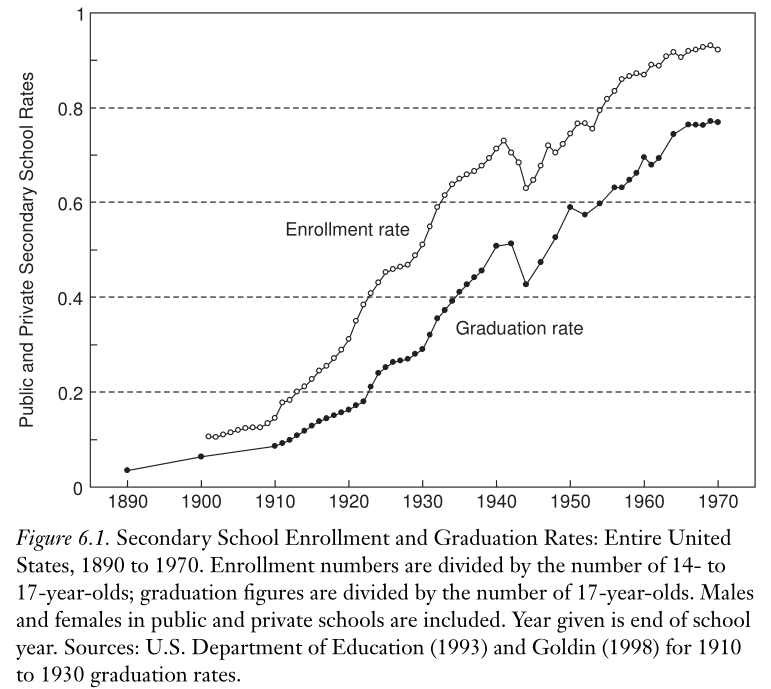
\includegraphics[clip, height = 8cm]{c:/seiro/docs/external/seishin/lec_slides/2024/HK/figure/GoldinKatzFigure61.jpg}
};
\coordinate (e1) at (.9, .6);
\node (a1) [ellipse, thick, rotate around = {48: (e1)}, minimum height = .5cm, minimum width = 2cm, fill = blue, draw=blue, fill opacity=.1] at (e1){};
\coordinate (e2) at ($(e1) + (2, 1.4)$);
\node (a2) [ellipse, thick, rotate around = {43: (e2)}, minimum height = .5cm, minimum width = 1.5cm, fill = blue, draw=blue, fill opacity=.1] at (e2){};
\end{tikzpicture}
\column{.25\paperwidth}
\end{columns}
\end{frame}

\begin{frame}[label=WhiteCollar]{}
\begin{columns}[T]
\column{.75\paperwidth}
ホワイトカラー職種の増加\citep[][Table 5.1]{GoldinKatz2009}\\ 
\begin{tikzpicture}[inner sep=0pt, remember picture]
\node at (0, 0) {
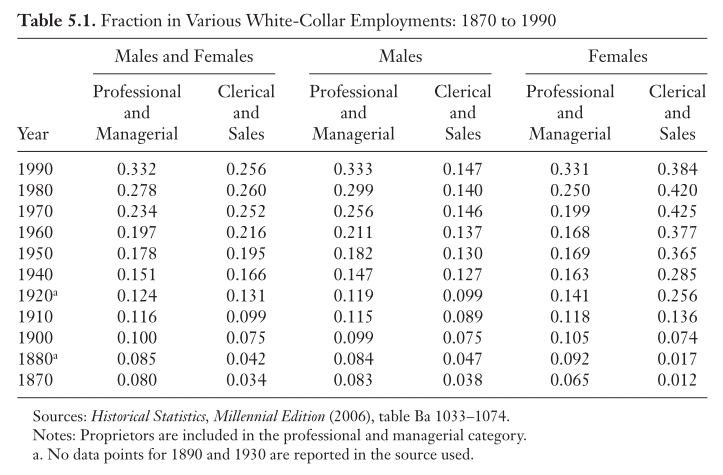
\includegraphics[clip, width = 10cm]{c:/seiro/docs/external/seishin/lec_slides/2024/HK/figure/GoldinKatzTable51.jpg}
};
\coordinate (h1) at (-2.0, -1.2);
\onslide<2->{
  \node (H1) [rectangle, anchor = south west, thick, rounded corners, minimum height = .5cm, 
    minimum width = .75cm, fill = blue, draw=blue, fill opacity=.1] at (h1){};
  \node (H2) [rectangle, anchor = south west, thick, rounded corners, minimum height = .5cm, 
    minimum width = .75cm, fill = blue, draw=blue, fill opacity=.1, yshift = .57cm] at (h1){};
}
\onslide<4->{
  \node (C1) [rectangle, anchor = south west, thick, rounded corners, minimum height = 1.25cm, 
    minimum width = .75cm, fill = red, draw=red, fill opacity=.1, xshift = -1.5cm, yshift = 1.1cm] at (h1){};
  \node (C2) [rectangle, anchor = south west, thick, rounded corners, minimum height = .6cm, 
    minimum width = .75cm, fill = red, draw=red, fill opacity=.1, xshift = 4.5cm, yshift = 1.7cm] at (h1){};
}
\end{tikzpicture}
\column{.25\paperwidth}
\begin{tikzpicture}[inner sep=0pt, remember picture]
\onslide<3->{\node (hh1) at (1, -3) {\mpage{.2\paperwidth}{\footnotesize 高卒者の増加}};}
\onslide<5->{\node (cc1) at (1, 0) {\mpage{.2\paperwidth}{\footnotesize 大卒者の増加}};}
\end{tikzpicture}
\begin{tikzpicture}[remember picture, overlay]
\onslide<3->{
  %\draw[red, very thick, ->] (hh1.west) .. controls +(-.1, -1.5) and +(-.5, -2.5) .. (H1.east);
  %\draw[red, very thick, ->] (hh1.west) .. controls +(-.1, -1.5) and +(-.5, -2.5) .. (H2.east);
  \draw[blue, very thick, latex-, ->] (hh1.west) to[out=200, in=10, looseness = 1] (H1.east);
  \draw[blue, very thick, latex-, ->] (hh1.west) to[out=200, in=10, looseness = 1] (H2.east);
  }
\onslide<5->{
  \draw[red, very thick, latex-, ->] (cc1.west) to[out=200, in=-10, looseness = 1] (C1.east);
  \draw[red, very thick, latex-, ->] (cc1.west) to[out=200, in=-10, looseness = 1] (C2.east);
}
\end{tikzpicture}

\end{columns}
\end{frame}

\begin{frame}[label=CollegeGraduates]{}
\begin{columns}[T]
\column{.75\paperwidth}
大学修了者の増加\citep[][Figure 7.1]{GoldinKatz2009}\\ 
\begin{tikzpicture}[inner sep=0pt, remember picture]
\node at (0, 0) {
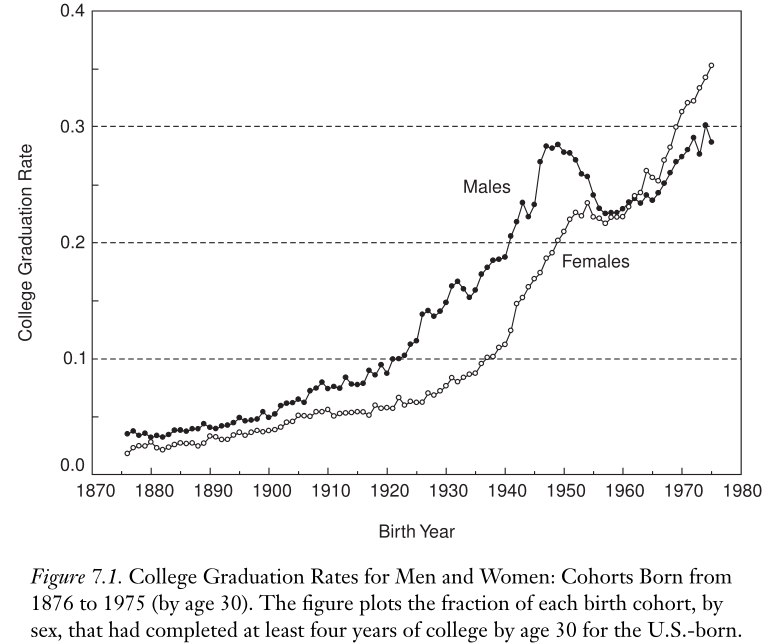
\includegraphics[clip, width = 10cm]{c:/seiro/docs/external/seishin/lec_slides/2024/HK/figure/GoldinKatzFigure71.jpg}
};
\coordinate (c1) at (3.9, 2.1);
\onslide<2->{\node (b1) [ellipse, thick, rotate around = {55: (c1)}, minimum height = .5cm, minimum width = 1.5cm, fill = red, draw=red, fill opacity=.1] at (c1){};}
\coordinate (c2) at ($(c1) + (0, .5)$);
\onslide<3->{\node (b2) [ellipse, thick, rotate around = {65: (c2)}, minimum height = .5cm, minimum width = 1.9cm, fill = red, draw=red, fill opacity=.1] at (c2){};}
\end{tikzpicture}
\column{.25\paperwidth}
\begin{tikzpicture}[inner sep=0pt, remember picture, text = white]
\onslide<2->{\node (CG1) at (0, 0) {\mpage{.2\paperwidth}{\footnotesize 男: ヴェトナム戦争兵役忌避といわれる}};}
\onslide<3->{\node (CG2) at (0, -3) {\mpage{.2\paperwidth}{\footnotesize 女: ? {\citet{GoldinKatz2009}} にも理由の記載なし。}};}
\end{tikzpicture}
\begin{tikzpicture}[remember picture, overlay]
\onslide<2->{\draw[red, very thick, ->] (CG1.south) .. controls +(-.1, -1.5) and +(-.5, -2.5) .. (b1.south);}
\onslide<3->{\draw[red, very thick, latex-, ->] (CG2.west) to[out=120, in=-10, looseness = 1] (b2.south east);}
\end{tikzpicture}

\end{columns}
\end{frame}

\begin{frame}{}
大卒需要の増加\citep[著者たちによる推計値][Table 8.1]{GoldinKatz2009}\\ 
\begin{columns}[T]
\column{.75\paperwidth}
\begin{tikzpicture}[inner sep=0pt, remember picture]
\node at (0, 0) {
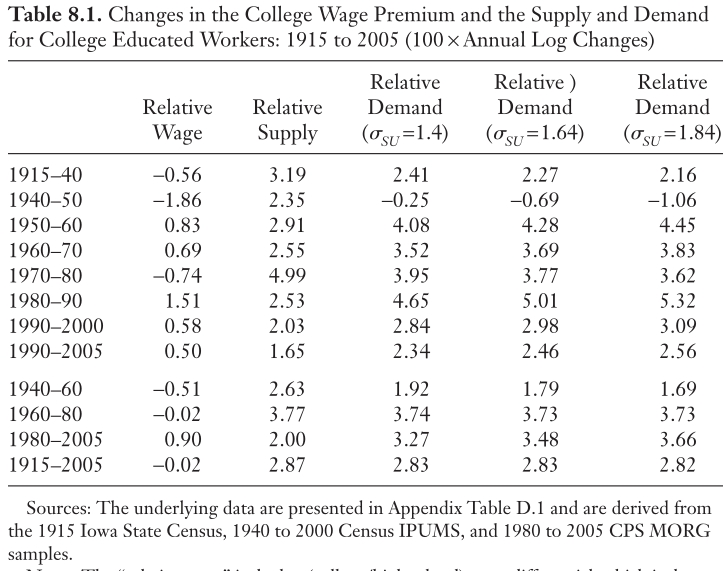
\includegraphics[clip, width = 10cm]{c:/seiro/docs/external/seishin/lec_slides/2024/HK/figure/GoldinKatzTable81.jpg}
};
\coordinate (c1) at (-3.0, -1.925);
\onslide<2->{\node (b1) [rectangle, thick, anchor = south west,  rounded corners, minimum height = .65cm, minimum width = 2.5cm, fill = blue, draw=blue, fill opacity=.1] at (c1){};}
\coordinate (c2) at ($(c1) + (0, -.35)$);
\onslide<3->{\node (b2) [rectangle, thick, anchor = south west,  rounded corners, minimum height = .3cm, minimum width = 2.5cm, fill = red, draw=red, fill opacity=.1] at (c2){};}
\end{tikzpicture}
\column{.25\paperwidth}
\begin{tikzpicture}[inner sep=0pt, remember picture]
\onslide<2->{\node (CG1) at (0, -1) {\mpage{.2\paperwidth}{\footnotesize 1940-80: 大卒賃金プレミアムは減少、供給の成長率高い}};}
\onslide<3->{\node (CG2) at (0, -3) {\mpage{.2\paperwidth}{\footnotesize 1980-2005: 大卒賃金プレミアムは増加、供給の成長率鈍化}};}
\end{tikzpicture}
\begin{tikzpicture}[remember picture, overlay]
\onslide<2->{\draw[blue, very thick, stealth-, ->] (CG1.west) to[out=180, in=90, looseness = 1]  (b1.north);}
\onslide<3->{\draw[red, very thick, stealth-, ->] (CG2.west) to[out=200, in=0, looseness = 1] (b2.east);}
\end{tikzpicture}

\end{columns}
\end{frame}

\begin{frame}{}
大卒賃金プレミアム vs. 高卒賃金プレミアム\citep[][Figure 8.1]{GoldinKatz2009}\\ 
\begin{columns}[T]
\column{.55\paperwidth}
\begin{tikzpicture}[inner sep=0pt, remember picture]
\node at (0, 1) {
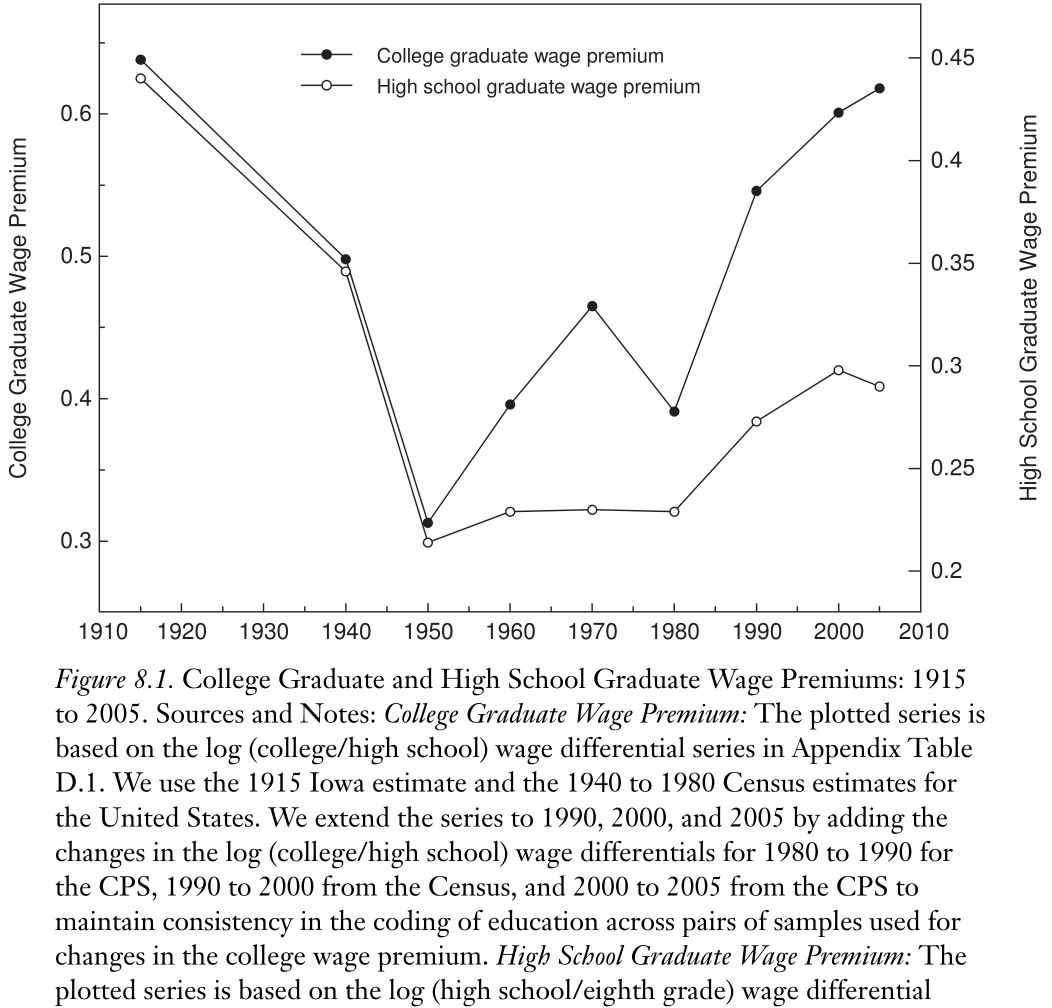
\includegraphics[clip, height = 8cm]{c:/seiro/docs/external/seishin/lec_slides/2024/HK/figure/GoldinKatz_Figure81.jpg}
};
\coordinate (c1) at (-.35, 1.1);
\onslide<2->{\node (b1) [ellipse, thick, anchor = south west, rotate around = {43: (c1)}, minimum height = .5cm, minimum width = 5.5cm, fill = red, draw=red, fill opacity=.1] at (c1){};}
\coordinate (c2) at ($(c1) + (0, -.4)$);
\onslide<3->{\node (b2) [ellipse, thick, anchor = south west, rotate around = {20: (c2)}, minimum height = .5cm, minimum width = 4.5cm, fill = orange, draw=orange, fill opacity=.1] at (c2){};}
\end{tikzpicture}
\column{.45\paperwidth}
\begin{tikzpicture}[inner sep=0pt, remember picture]
\onslide<2->{\node (CG1) at (0, 0) {\mpage{.45\paperwidth}{\footnotesize A race between education and skill-biased technological change.}};}
\onslide<3->{\node (CG2) at (0, -2) {\mpage{.45\paperwidth}{\footnotesize 競争: \\
\hfil 教育水準増加による技能の供給増加\\
\hfil vs. \\
\hfil 技能偏向的技術変化による技能の需要増加}};}
\onslide<4->{\node (CG3) at (0, -5) {\mpage{.45\paperwidth}{\footnotesize 供給の負け}};}
\end{tikzpicture}
\begin{tikzpicture}[remember picture, overlay]
\onslide<4->{\draw[red, very thick, arrows={latex-}, ->] (CG3.west) to[out=150, in=0, looseness = 1] (b1.south east);}
\end{tikzpicture}

\end{columns}
\end{frame}

\begin{Schunk}
\begin{Soutput}
Warning in grep(str, x, perl = T): input string 2 is invalid UTF-8
\end{Soutput}
\begin{Soutput}
Warning in grep(str, x, perl = T): input string 4 is invalid UTF-8
\end{Soutput}
\begin{Soutput}
Warning in grep(str, x, perl = T): input string 6 is invalid UTF-8
\end{Soutput}
\begin{Soutput}
Warning in grep(str, x, perl = T): input string 8 is invalid UTF-8
\end{Soutput}
\begin{Soutput}
Warning in grep(str, x, perl = T): input string 10 is invalid UTF-8
\end{Soutput}
\begin{Soutput}
Warning in grep(str, x, perl = T): input string 1 is invalid UTF-8
\end{Soutput}
\begin{Soutput}
Warning in grep(str, x, perl = T): input string 2 is invalid UTF-8
\end{Soutput}
\begin{Soutput}
Warning in grep(str, x, perl = T): input string 3 is invalid UTF-8
\end{Soutput}
\begin{Soutput}
Warning in grep(str, x, perl = T): input string 4 is invalid UTF-8
\end{Soutput}
\begin{Soutput}
Warning in grep(str, x, perl = T): input string 5 is invalid UTF-8
\end{Soutput}
\begin{Soutput}
Error in if (ncol(nn) != 2L) stop("failed to guess time-varying variables from their names"): 引数の長さが 0 です
\end{Soutput}
\begin{Soutput}
Error in eval(expr, envir, enclos): オブジェクト 'shL' がありません
\end{Soutput}
\begin{Soutput}
Error in eval(expr, envir, enclos): オブジェクト 'shL' がありません
\end{Soutput}
\begin{Soutput}
Error in eval(expr, envir, enclos): オブジェクト 'shL' がありません
\end{Soutput}
\begin{Soutput}
Error in eval(expr, envir, enclos): オブジェクト 'shL' がありません
\end{Soutput}
\begin{Soutput}
Error in eval(expr, envir, enclos): オブジェクト 'shL' がありません
\end{Soutput}
\begin{Soutput}
Error in eval(expr, envir, enclos): オブジェクト 'shL' がありません
\end{Soutput}
\begin{Soutput}
Error in eval(expr, envir, enclos): オブジェクト 'shLL' がありません
\end{Soutput}
\begin{Soutput}
Error in eval(expr, envir, enclos): オブジェクト 'shLL' がありません
\end{Soutput}
\end{Schunk}


\begin{frame}{}
技能の高い人口が増えると技術が開発され、採用され、(高)技能労働への需要が増える
\begin{itemize}
\vspace{1.0ex}\setlength{\itemsep}{1.0ex}\setlength{\baselineskip}{12pt}
\item	技術変化には特定の生産要素(労働、資本など)をより多く使う方向性がある(特定生産要素を増減する方向性のある技術変化をdirected technical changeといいます)
\item	理由: (高)技能人口が増えると、技術開発をして技術を売る企業にとって(高)技能偏向的技術開発の利潤が高まるため\citep{Acemoglu2002}
	\begin{dinglist}{43}
	\vspace{1.0ex}\setlength{\itemsep}{1.0ex}\setlength{\baselineskip}{12pt}
	\item	価格効果: (高)技能人口が増えると、相対的に稀少になった(低技能)労働を多く使う財の価格が高くなるので、(低技能)労働偏向的技術が開発される
	%希少な生産要素を用いる技術の開発
	\item	市場規模効果: (高)技能偏向的技術を使う財の市場規模が大きければ、(高)技能偏向的技術が開発される
	%より潤沢な生産要素を用いる市場規模の大きい技術の開発
	\item	殆どの場合、市場規模効果は価格効果を上回るので、(高)技能人口が増えると(高)技能偏向的技術が多くなる
	%\item	高技能労働が増えると価格効果によって希少でなくなった高技能労働賃金が下がるが、市場規模効果によって潤沢になった高技能労働賃金は増える。低技能労働から高技能労働への代替を弱く促進する(代替弾力性が2よりも大きい)とき、市場規模効果が支配的になる。
	\end{dinglist}
\end{itemize}
\end{frame}

\begin{frame}{}
技能偏向的技術変化があるとき\\~\\
\pause
人的資本投資へのアクセスが容易で技能労働供給が潤沢ならば、賃金格差は減りつつ経済成長が高まる\\~\\
\pause
人的資本投資へのアクセスが一部のみが可能であれば、技能労働供給が限られ、賃金格差は増えつつ経済成長が低迷する
\begin{dinglist}{43}
\vspace{1.0ex}\setlength{\itemsep}{1.0ex}\setlength{\baselineskip}{12pt}
\pause
\item	1980-2005年: 大卒賃金プレミアム
\begin{description}
\vspace{1.0ex}\setlength{\itemsep}{1.0ex}\setlength{\baselineskip}{12pt}	
\item[拡大]	アメリカ、イギリス、日本(プレミアム水準はアメリカの半分)
\item[変化なし]	フランス、ドイツ\\[2ex]
\end{description}
\end{dinglist}
\pause
アメリカで大卒人口が増えないのは教育産業の容量上限ではない
\begin{dinglist}{43}
\vspace{1.0ex}\setlength{\itemsep}{1.0ex}\setlength{\baselineskip}{12pt}
\pause
\item	他国では増えている
\pause
\item	高校ドロップアウトや高卒の学力が不足\citep[][p.347]{GoldinKatz2009}
\pause
\item	大学の学費が高騰、ベビーブーマー世代が大学学齢になったとき奨学金が不足=credit constrained\citep[][p.349]{GoldinKatz2009}
\end{dinglist}
\end{frame}

\begin{frame}{}
日本の大学賃金プレミアム(新卒初任給)\\
\hfil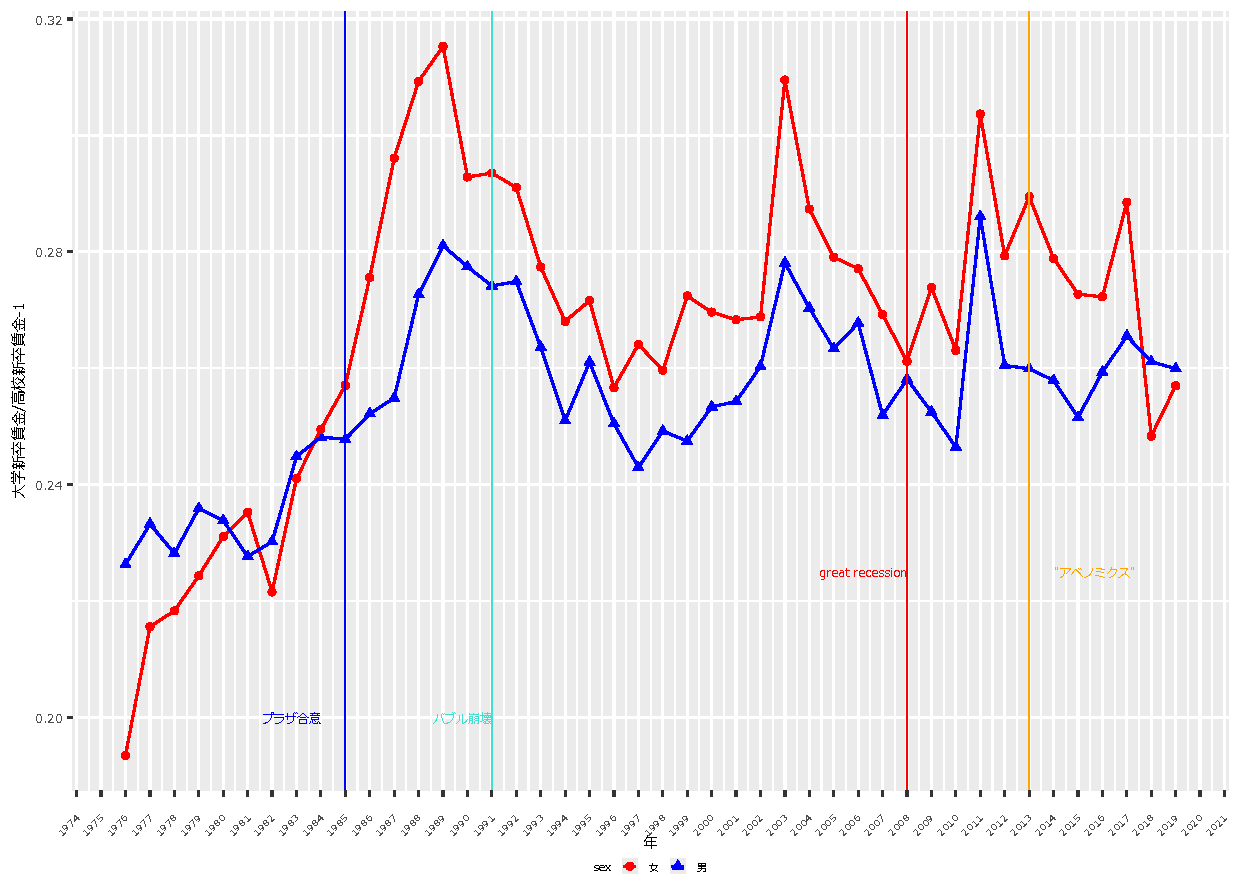
\includegraphics[clip, height = 7.5cm]{c:/seiro/docs/external/seishin/lec_slides/2024/HK/figure/CollegePremiumInJapan.pdf}\\
{\footnotesize 出所: 厚生労働省「賃金構造基本統計調査」第1表(企業規模別新規学卒者の初任給の推移)}
\end{frame}



\begin{frame}{}
アメリカの所得分配\\
\begin{columns}[T]
\column{.75\paperwidth}
\begin{tikzpicture}[inner sep=0pt, remember picture, text = white]
\node at (0, 1) {
\hfil\mpage{.75\paperwidth}{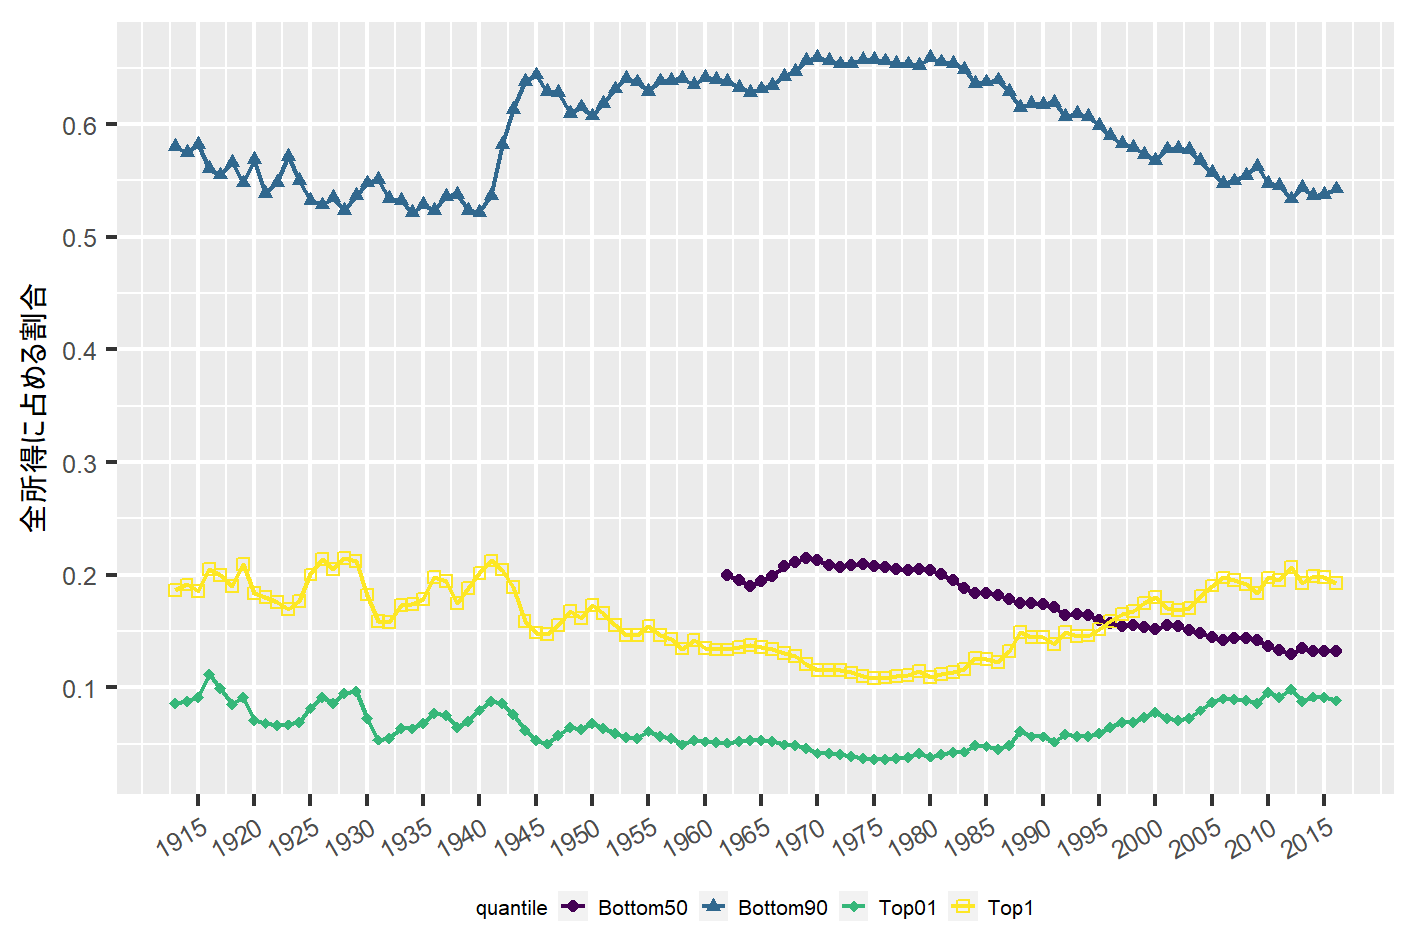
\includegraphics[height = 7.5cm, width = 12cm]{c:/seiro/docs/external/seishin/lec_slides/2022/HK/figure/PikettySaezZucman_IncomeDistribution.png}\\
{\footnotesize 出所: \citet[][Table TB1]{PikettySaezZucman2018}より作成。}
}
};
\coordinate (c1) at (2.2, 4.25);
\onslide<2, 3>{\node (b1) [ellipse, thick, anchor = south west, rotate around = {-18: (c1)}, minimum height = .5cm, minimum width = 4.0cm, fill = red, draw=red, fill opacity=.1] at (c1){};}
\coordinate (c2) at ($(c1) + (0, -4.0)$);
\onslide<3>{\node (b2) [ellipse, thick, anchor = south west, rotate around = {-11: (c2)}, minimum height = .5cm, minimum width = 4.0cm, fill = red, draw=red, fill opacity=.1] at (c2){};}
\coordinate (c3) at ($(c1) + (0, -4.7)$);
\coordinate (c4) at ($(c1) + (0, -5.4)$);
\onslide<4>{
  \node (b3) [ellipse, thick, anchor = south west, rotate around = {13: (c3)}, minimum height = .5cm, 
    minimum width = 4.0cm, fill = orange, draw=orange, fill opacity=.1] at (c3){};
  \node (b4) [ellipse, thick, anchor = south west, rotate around = {9: (c4)}, minimum height = .5cm, 
    minimum width = 4.0cm, fill = orange, draw=orange, fill opacity=.1] at (c4){};
}
\coordinate (c5) at ($(c1) + (-4, -1.0)$);
\coordinate (c6) at ($(c1) + (-4.2, -3.8)$);
\coordinate (c7) at ($(c1) + (-4.2, -4.8)$);
\onslide<5>{
  \node (b5) [ellipse, thick, anchor = south west, rotate around = {70: (c5)}, minimum height = .5cm, 
    minimum width = 1.5cm, fill = blue, draw=blue, fill opacity=.1] at (c5){};
  \node (b6) [ellipse, thick, anchor = south west, rotate around = {-55: (c6)}, minimum height = .5cm, 
    minimum width = 1.0cm, fill = blue, draw=blue, fill opacity=.1] at (c6){};
  \node (b7) [ellipse, thick, anchor = south west, rotate around = {-45: (c7)}, minimum height = .5cm, 
    minimum width = 1.0cm, fill = blue, draw=blue, fill opacity=.1] at (c7){};
}
\coordinate (c8) at ($(c1) + (-5.25, -0.9)$);
\coordinate (c9) at ($(c1) + (-5.4, -3.8)$);
\coordinate (c10) at ($(c1) + (-5.4, -4.8)$);
\onslide<6>{
  \node (b8) [ellipse, thick, anchor = south west, rotate around = {-10: (c8)}, minimum height = .5cm, 
    minimum width = 0.8cm, fill = purple, draw=purple, fill opacity=.1] at (c8){};
  \node (b9) [ellipse, thick, anchor = south west, rotate around = {-55: (c9)}, minimum height = .5cm, 
    minimum width = 0.8cm, fill = purple, draw=purple, fill opacity=.1] at (c9){};
  \node (b10) [ellipse, thick, anchor = south west, rotate around = {-45: (c10)}, minimum height = .5cm, 
    minimum width = 0.8cm, fill = purple, draw=purple, fill opacity=.1] at (c10){};
}
\coordinate (c11) at ($(c1) + (-4.2, -0.9)$);
\coordinate (c12) at ($(c1) + (-4.2, -3.8)$);
\coordinate (c13) at ($(c1) + (-4.2, -4.8)$);
\onslide<7>{
  \draw [blue] (c11) --  ($(c11)+(7.5, 0)$){};
  \draw [blue] (c12) --  ($(c12)+(7.5, 0)$){};
  \draw [blue] (c13) --  ($(c13)+(7.5, 0)$){};
}
\end{tikzpicture}
\column{.20\paperwidth}
\begin{tikzpicture}[inner sep=0pt, remember picture]
\node (CG1) at (0, 0) {\mpage{.20\paperwidth}{\footnotesize \onslide<2->{1980年以降: 下位のシェアが低下}\onslide<4->{、上位のシェアが上昇}}};
\onslide<5->{\node (CG2) at (0, -2) {\mpage{.20\paperwidth}{\footnotesize 1940-45年: 大戦期は平等化}};}
\onslide<6->{\node (CG3) at (0, -4) {\mpage{.20\paperwidth}{\footnotesize 1929年、2008年以後数年: 経済危機は平等化}};}
\onslide<7->{\node (CG4) at (0, -6) {\mpage{.20\paperwidth}{\footnotesize 2010年以降: 上位のシェアは第2次大戦直前水準に近い}};}
\end{tikzpicture}
\begin{tikzpicture}[remember picture, overlay]
\onslide<3>{
\draw[red, very thick, arrows={latex-}, ->] (CG1.west) to[out=200, in=40, looseness = 1] (b1.north east);
\draw[red, very thick, arrows={latex-}, ->] (CG1.west) to[out=200, in=40, looseness = 1] (b2.north east);
}
\onslide<4>{
\draw[orange, very thick, arrows={latex-}, ->] (CG1.south west) to[out=200, in=90, looseness = 1] (b3.north east);
\draw[orange, very thick, arrows={latex-}, ->] (CG1.south west) to[out=200, in=40, looseness = 1] (b4.east);
}
\end{tikzpicture}
\end{columns}
\end{frame}

\begin{frame}[label=InequalityInTwoSense]{}
近年の格差: MITのDavid Autor\href{https://economics.mit.edu/people/faculty/david-h-autor/courses}{労働経済学講義14.662 Lecture 1スライド}を引用
\begin{itemize}
\vspace{1.0ex}\setlength{\itemsep}{3.0ex}\setlength{\baselineskip}{12pt}
\item	所得
	\begin{itemize}
	\vspace{1.0ex}\setlength{\itemsep}{1.0ex}\setlength{\baselineskip}{12pt}
	\item	所得格差拡大[6, 8]、中間層の縮小[9]、トップ層の超富裕化[61, 68]、賃金格差拡大[12, 15-21]、世代間可動性低下[23]、低所得層の固定化[27]
	\item	大卒プレミアム上昇[48]、大卒賃金プロファイルのフラット化[58-59]
	\item	職業2極化occupational polarization[50, 52, 54]
	\end{itemize}
\item	資産 [69, 74]
\end{itemize}

\end{frame}
\begin{frame}[label=InequalityHypothesises]{}
近年の格差の原因: 諸仮説
\begin{description}
\vspace{1.0ex}\setlength{\itemsep}{1.0ex}\setlength{\baselineskip}{12pt}
\pause
\item[技能労働需給]		技能偏向的技術変化、技能労働需要の高まりに比して技能労働供給が少なかったため\citep{KatzMurphy1992, GoldinKatz2009}。人的資本投資補助。$\leftarrow$近年ではAIやロボットがルーティーン作業の職種を代替し中間層が減り、さらに、大卒の賃金プロファイルもフラット化
\pause
\item[資本収益率が高い]	資本収益率が経済成長率よりも高いために資産が集中する\citep{Piketty2014}。相続資産収益率は富裕層が高くその他層は費消するので、相続を通じて資産格差が拡大\citep{NekoeiSeim2022}。資産への累進課税。
\pause
\item[階級的特権]	あまり詳細に示しておらず、さまざまな原因を挙げているが、教育アクセスの差を重要視\citep{Piketty2014}。1980年代半ば以降、トップ0.1\%、1\%が資産所得と経営者報酬で所得急増、高額所得者の実効税率の低下、課税逃れなど\citep{PikettySaez2014,PikettySaezZucman2018}。教育機会の均等や資産への累進課税。
\pause
\item[スーパースター企業の成長]	大企業が成長しスーパースター企業となり、その他の企業は市場シェアを落とした。生産のシェアが高まったスーパースター企業の労働分配率は低いので、平均労働所得増加率が減った\citep{ADKPV2020}。スーパースター企業の所有者は富を得たが、それ以外はじり貧。
%\pause
%\item[社会的隔離social segregation]	特定グループ(学校、地縁、職業など)への所属membership \citep{Durlauf1996}。他グループとの交流を促す政策(学区変更、授業料ヴァウチャー制度など)を推奨。
\end{description}
\end{frame}


\begin{frame}{}
先進国では人的資本投資の停滞や労働需要の質変化が格差の原因として考えられる\\~\\
\pause
アメリカなど(先進国)では高等教育へのアクセスが不十分なために高技能供給が停滞\\~\\
\pause
1980年代以降の技能偏向的技術進歩による高技能需要の高まりが高技能供給停滞と相まって高技能賃金を高め、高技能保有者とそれ以外の格差を拡大\\~\\
\pause
2000年前後の対策: 高技能供給を増やすことが格差縮小手段の1つのはずだった\\~\\
\pause
現在: アルゴリズム化できる技能codifiable skillsはAIに代替されるため、高技能でもアルゴリズム化しにくい内容という制約が加わった\\~\\
\pause
技能偏向的でデータ集約的技術進歩で求められる技能=AIとAIが用いるデータを補完する高技能、であれば、データ集約的な技術進歩とともに労働需要が高まる
\end{frame}

\begin{frame}{}
途上国の場合、自国で技術開発されることは少なく、多くが輸入された技術\\~\\
\pause
\citet{JerzmanowskiTamura2019}: 各国の技能別人口データを使って推計
\begin{itemize}
\vspace{1.0ex}\setlength{\itemsep}{1.0ex}\setlength{\baselineskip}{12pt}
\pause
\item	途上国は人口の技能に準じた技術を導入していないために成長が遅い
\pause
\item	途上国は人口の技能水準をアメリカと同じまで引き上げるよりも、現在の技能水準にあった技術を導入する方が所得の増加幅が大きい\\~\\
\end{itemize}
\pause
\citet{Okoye2016}: 「適正技術論」の内容(途上国は低技能労働者に適正な技術を採用していないので変えるべき)は現実と逆
\begin{itemize}
\vspace{1.0ex}\setlength{\itemsep}{1.0ex}\setlength{\baselineskip}{12pt}
\pause
\item	技能労働者の物的環境は先進国より途上国の方が劣悪
\pause
\item	技能労働者の物的環境を改善する技術変化で所得を増やせる
\pause
\item	つまり、途上国は低技能労働者を優先し過ぎた技術を採用している
\pause
\item	技能労働者の物的環境を改善する技術が採用されない理由: 既得権益、資本市場の失敗、インフラストラクチュア未整備$\leftarrow$証拠なしで議論\\~\\
\end{itemize}
\pause
政府による政策選択が違いをもたらすかもしれない
\end{frame}

\begin{frame}{}
\textcolor{azure}{中国:} 準技能の低賃金労働に適した大量生産技術=FDI
\begin{dinglist}{43}
\vspace{1.0ex}\setlength{\itemsep}{1.0ex}\setlength{\baselineskip}{12pt}
\pause
\item	貧困層の所得を増やしつつ成長
\end{dinglist}
\vspace{1ex}
\pause
最近では賃金上昇と需要の細分化(多品種少量生産): 生産の自動化\\~\\
\pause
\textcolor{azure}{インド:} 自由化(1991年)後も保護・規制を継続、交通・エネルギーのインフラ整備不足、準技能英語使用の低賃金労働に適した技術
\begin{dinglist}{43}
\vspace{1.0ex}\setlength{\itemsep}{1.0ex}\setlength{\baselineskip}{12pt}
\pause
\item	コールセンター、会計、ICT設計など都市部でのサービス業務オフショア化労働需要
\pause
\item	技能供給: 農村部公立教育はダメ、農村部私立教育も大差ない
\end{dinglist}
\vspace{2ex}
\pause
\textcolor{azure}{南アフリカ:} 解雇の難しい低技能の中賃金労働、高技能の白人層
\begin{dinglist}{43}
\vspace{1.0ex}\setlength{\itemsep}{1.0ex}\setlength{\baselineskip}{12pt}
\pause
\item	現場監督の技能の需要が高まる
\pause
\item	高校教育: 質の格差が大きく、労働市場で高卒の評価は低い
\pause
\item	大学教育の収益率は初等教育や中等教育よりも高い
\pause
\item	格差を減らしながらの成長は難しい
\end{dinglist}
\end{frame}

\begin{frame}{}
\citet{BalandRobinson2000} model relates to MDGs (Milleneum Development Goals) and SDGs (Sustainable Development Goals)\\ 
\hfil\begin{columns}[T]
\column{.4\paperwidth}
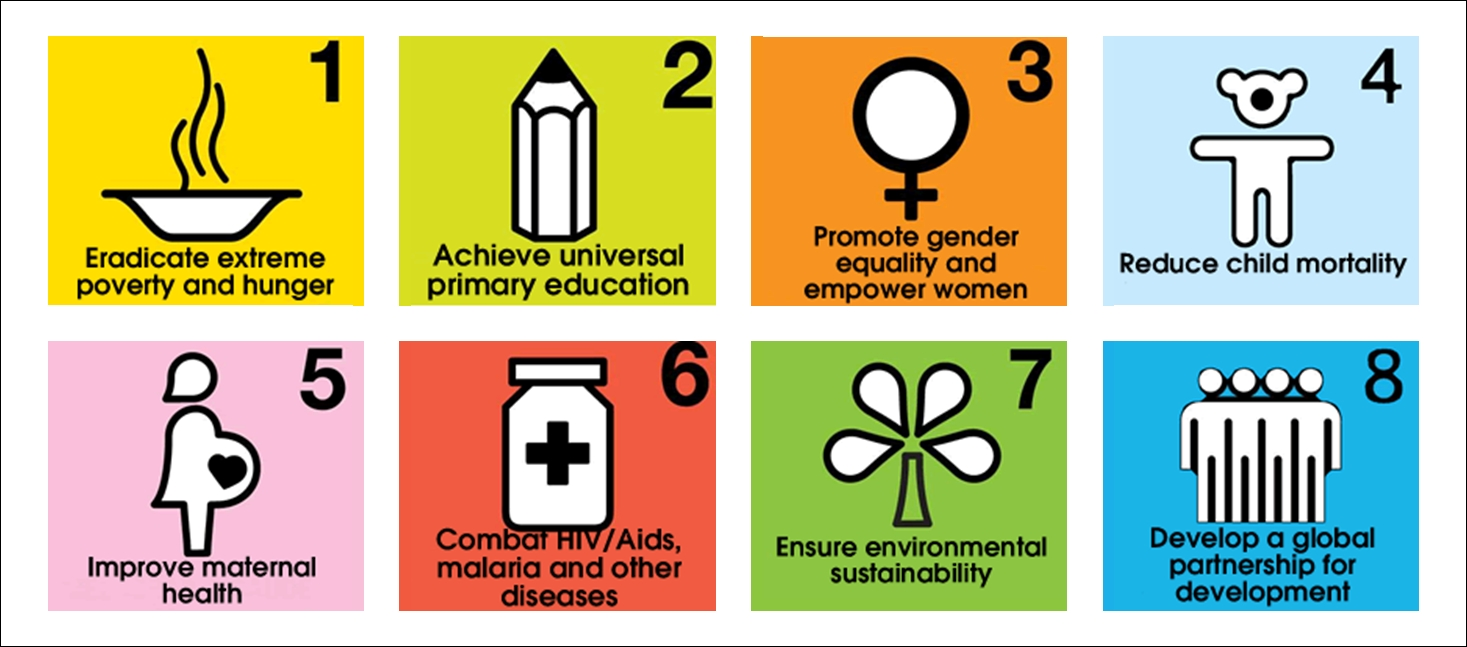
\includegraphics[clip, width = .4\paperwidth]{c:/seiro/docs/external/seishin/lec_slides/2024/HK/figure/MDG.jpg}
\column{.4\paperwidth}

\includegraphics[clip, height = .35\paperheight]{c:/seiro/docs/external/seishin/lec_slides/2024/HK/figure/SDGs.jpg}
\end{columns}

\vspace{2ex}
\pause
「(成長過程に参加して)豊かになる手段としての人的資本投資」で考えるべきこと
\begin{itemize}
\vspace{1.0ex}\setlength{\itemsep}{1.0ex}\setlength{\baselineskip}{12pt}
\pause
\item	どの学歴水準を得るか(初等教育までならばMDGs)
\pause
\item	その学歴で得られる技能水準はどれくらいか(SDGs)
\pause
\item	その技能水準への労働需要は高いか\pause
 $\leftarrow$ なかなか議論されない
\end{itemize}
\end{frame}

\begin{frame}{}
SDGs: 質の高い教育機会を保証することに留まり、どこまで技能を得れば最適か(生涯効用が最大化するか)は議論していない\\~\\
政府は、進学しそうな人数、進学してほしい人数を想定して、教育機会を供給するはず%\\~\\
%進学を考える人数は、(個人が合理的ならば)技能別労働需要の展望に依存するはず
\begin{dinglist}{43}
\vspace{1.0ex}\setlength{\itemsep}{1.0ex}\setlength{\baselineskip}{12pt}
\pause
\item	技能形成は積み上げなので、初等教育の質が低ければ中等教育も頓挫する
\pause
\item	順番: 幅広く質の高い初等教育、次いでの幅広さで質の高い中等教育を供給できるか
\pause
\item	質の高い教育機会の提供方法は?
\end{dinglist}
\end{frame}

\begin{frame}{}
India: Rights to Education Act (April, 2010)\\
\pause
Free and compulsory education. Obligation of Central and State governments.\\~\\
\pause
Affirmative action: Makes a provision for any school to admit low caste children.\\~\\

\pause
What happened after RTE?\\~\\

\pause
Classes were flooded with children, even after constructing new schools. \pause Many schools had to run multi grade classes.\\~\\
\pause
Requirements for unlicensed private schools to satisfy facility requirements led to closure schools. Wow.\\~\\
\pause
It is good to send children to schools. \\~\\
\pause
Only if they are learning.
\end{frame}

\begin{frame}{}
\begin{columns}[T]
\column{.75\paperwidth}
\mpage{.75\paperwidth}{
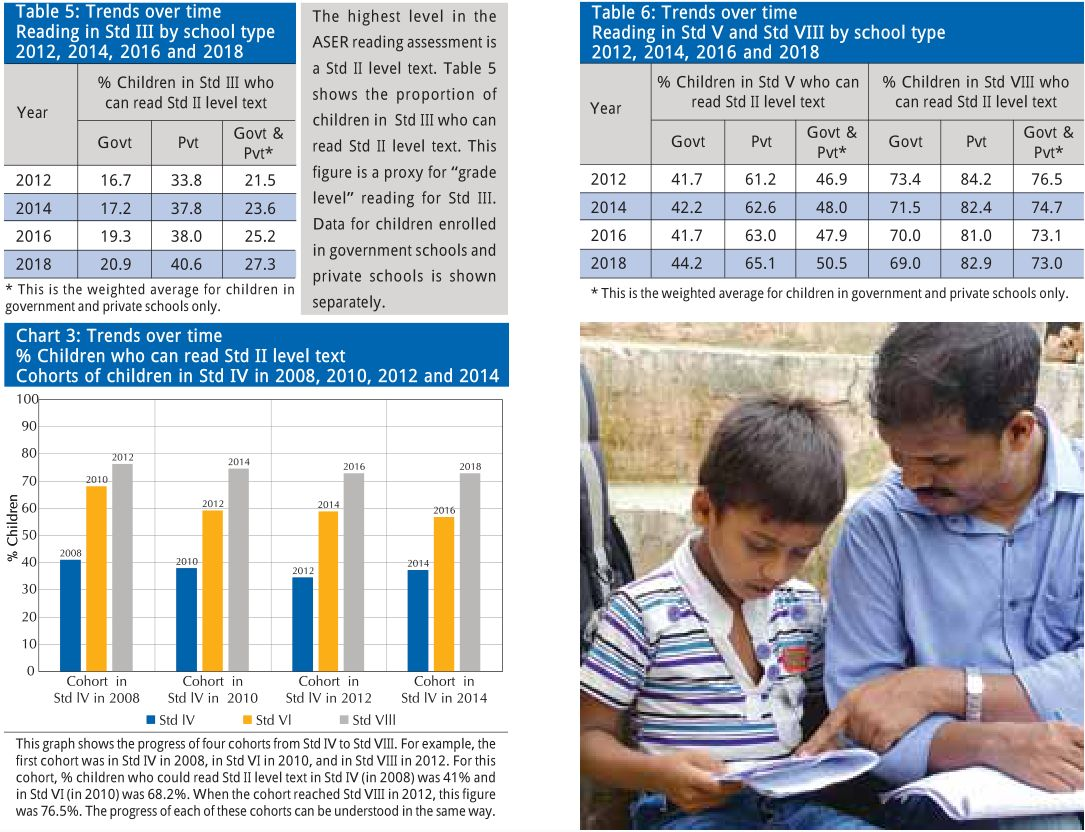
\includegraphics[width = .375\paperwidth]{HK/figure/Pratham2018GovPvtReading.jpg}
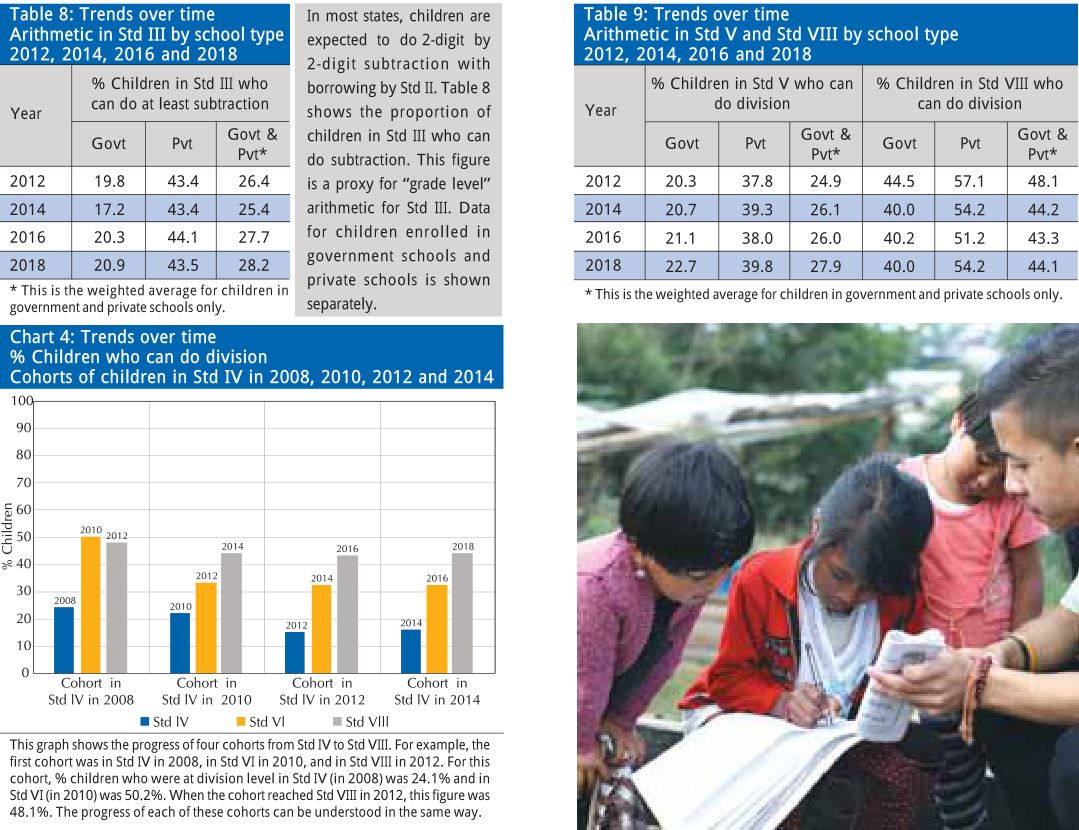
\includegraphics[width = .375\paperwidth]{HK/figure/Pratham2018GovPvtArithmetic.jpg}\\
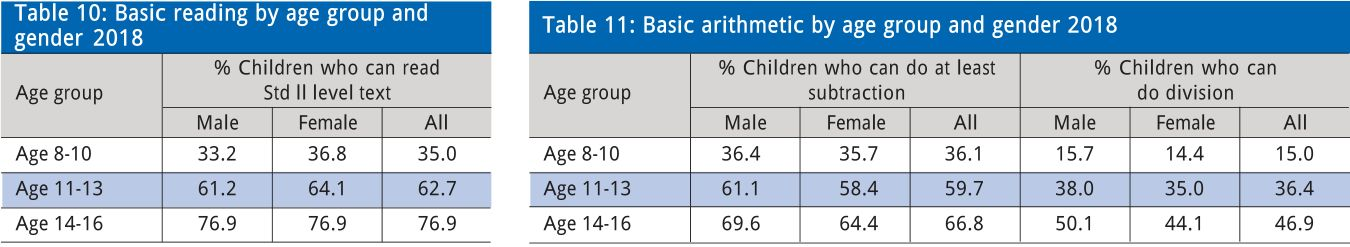
\includegraphics[width = .75\paperwidth]{HK/figure/Pratham2018Gender.jpg}\\
\vspace{-1ex}出所: \citet[][p.52-54]{Pratham2018}
}
\column{.175\paperwidth}\footnotesize
進級しているが、学力が伴っていない。公立、私立、男女、いずれも低い。\\~\\

SDGs04: Quality education for everyone質の高い教育をみんなに
\end{columns}
\end{frame}


\begin{frame}{}

If the governments are sending children to schools, they must provide quality.\\~\\
\pause
With low quality education, more child labour may become efficient.\\~\\
\pause
Does paying teachers for the performance result in more learning?
\end{frame}

\begin{frame}[t]{}
学力を上げることを目的とした政策
\begin{columns}[T]
\column{.65\paperwidth}
\begin{itemize}
\vspace{1.0ex}\setlength{\itemsep}{1.0ex}\setlength{\baselineskip}{12pt}
\item	\textcolor{green}{家計への補助金(無条件、条件付き)、授業料ヴァウチャー、学校給食}
\item	保護者への情報伝達(学校の成績、教育投資の収益性)
\item	奨励金student incentives
\item	\textcolor{green}{教材、施設、教員数を拡充}
\item	\textcolor{azure}{学級規模class sizeの縮小}
\item	教授法改善(tracking, ICT assisted learning)
\item	\textcolor{green}{教員再訓練}
\item	\textcolor{green}{教員の出勤徹底}
\item	\textcolor{green}{教員給与の成果報酬制(pay for performance)}
\item	学校の経営自由度上昇、保護者の経営参加
\item	学校間競争、私立学校設立奨励
\end{itemize}
\column{.3\paperwidth}
\pause
低所得国で問題になるのは学校へのアクセス(就学)、教材や施設の不足、教員数不足や怠業、教員の能力や努力\\~\\
\pause
\textcolor{green}{RCTで実験しやすい}のは家計への補助金、ヴァウチャー、給食、知識伝達、予算、再訓練、成果報酬など
\end{columns}
\end{frame}

\begin{frame}[t, label=MbitiFirstPage]{}
\citet{Mbiti2019}: 学力を高めるためには何と何が必要か?
\begin{itemize}
\vspace{1.0ex}\setlength{\itemsep}{1.0ex}\setlength{\baselineskip}{12pt}
\item	先生の能力や努力$\leftarrow$成果報酬(ボーナス, pay for performance, P4P) 
\item	教材や施設など$\leftarrow$学校予算\\[2ex]
\end{itemize}
\pause
タンザニアでの実験(2013-2014年): 公立学校350校(生徒数12万人)%$\leftarrow$1学年あたり57人!
\begin{itemize}
\vspace{1.0ex}\setlength{\itemsep}{1.0ex}\setlength{\baselineskip}{12pt}
\item	全国10郡で35校を無作為抽出random sample、小学1-3年生
\item	全国を代表する標本
\pause
\item	70校: 学校予算増額(生徒1人あたりUSD6.25, 教科書4-5冊分)
\item	70校: 先生の成果報酬(試験合格人数$\times$USD3、校長はUSD.6)$\leftarrow$やや効果あり
\item	70校: 学校予算増額と先生の成果報酬$\leftarrow$効果あり
\item	140校: 統御群control group(介入なし)=処置群treated groupの比較対象
\end{itemize}
\end{frame}

\begin{frame}[t, label=MbitiResults]{}
\begin{columns}[T]
\column{.75\paperwidth}
\begin{tikzpicture}[inner sep=0pt, remember picture]
\node at (0, 0) {
\mpage{.75\paperwidth}{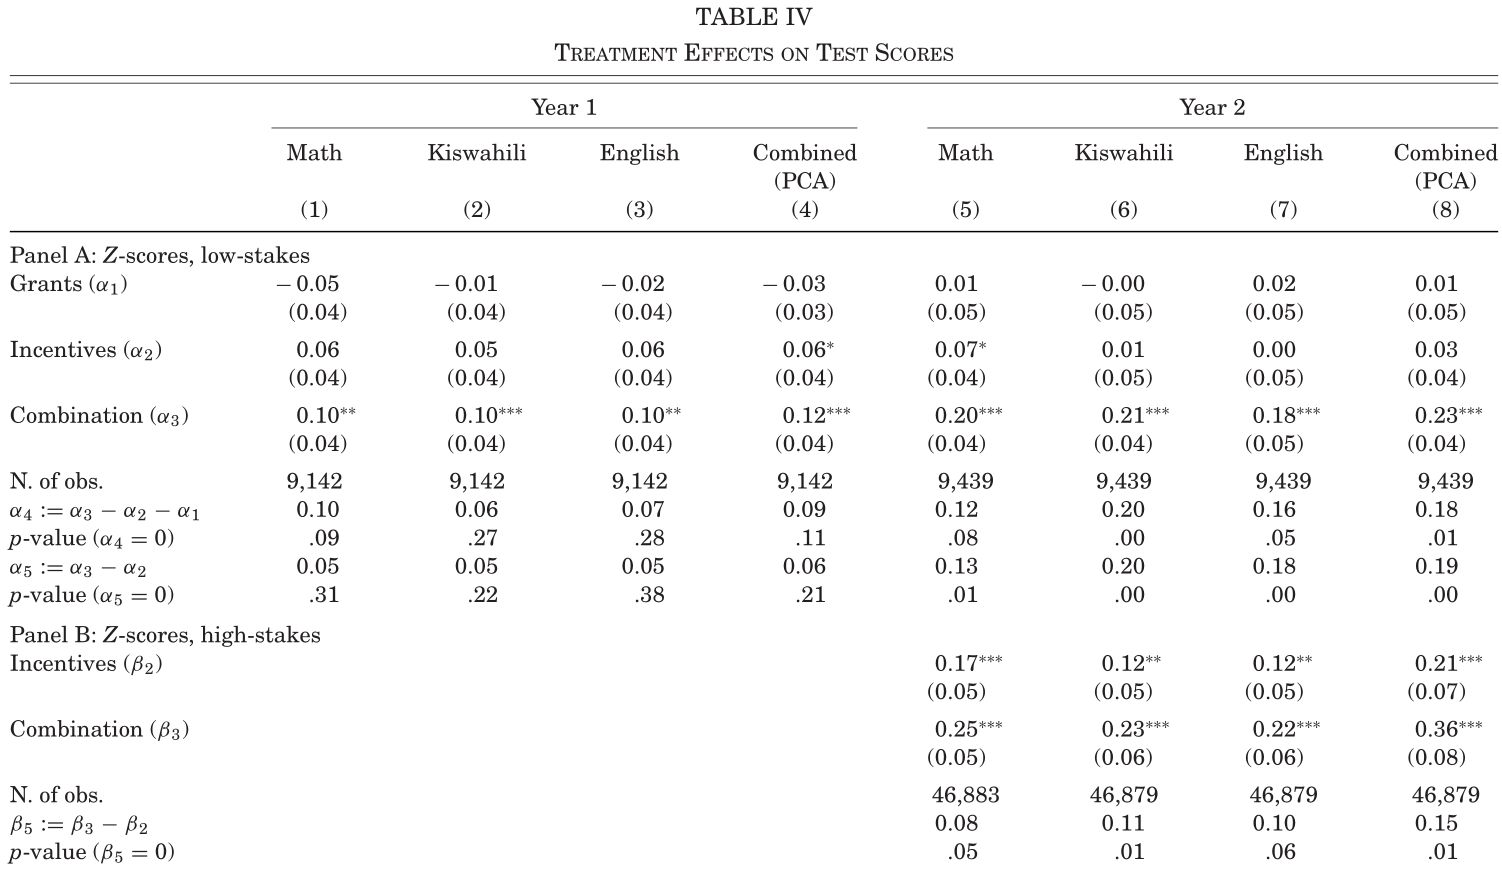
\includegraphics[width = .75\paperwidth]{HK/figure/Mbiti_Tab4.jpg}\\
\vspace{-1ex}{\footnotesize 出所: \citet[][1650-1651]{Mbiti2019}}}
};
\onslide<2->{\node (a1) [rectangle, thick, rounded corners, minimum height = .5cm, minimum width = .75\paperwidth, fill = red, draw=red, fill opacity=.1] at (0cm, .22cm){};}
\onslide<4->{\node (a2) [rectangle, thick, rounded corners, minimum height = .5cm, minimum width = .75\paperwidth, draw=blue, fill = blue, fill opacity=.1, below of = a1, yshift = .25cm]{};}
\end{tikzpicture}
\column{.2\paperwidth}
\begin{tikzpicture}[inner sep=0pt, remember picture]
\node (b0) at (0, 0) {\mpage{.2\paperwidth}{\footnotesize \mpagethree{.12\paperwidth}{\hfil 点推計値\\\hfil (標準誤差)}{c} 表示}};
\onslide<3->{\node (b1) at (0, -1.5) {\mpage{.2\paperwidth}{\footnotesize 予算+成果報酬で効果あり}};}
\onslide<5->{\node (b2) at (0, -5) {\mpage{.2\paperwidth}{\footnotesize $\alpha_{4}=$Combination\\
-Grant-Incentives=0、つまり、帰無仮説「両方は片方ずつの合計と同じ」の検定。p-valueは帰無仮説が成立する確率。「両方付与すると片方ずつの合計よりも大きくない」確率が(8)では1\%。}};}
\end{tikzpicture}
\begin{tikzpicture}[remember picture, overlay]
\onslide<3->{\draw[red, very thick, ->] (b1.west) to [out=180, in=90] (a1.north);}
\onslide<5->{\draw[blue, very thick, ->] (b2.west) to [out=180, in=-90] (a2.south);}
\end{tikzpicture}
\end{columns}
\end{frame}

\begin{frame}[t]{}
なぜ両方必要なのか?\\~\\
\citet{Mbiti2019}は理論モデルを作って、どのような性質の教員であれば、予算、成果報酬の単体では学力が上がらず、両方あるときにのみ学力が上がるか、理論的可能性を分析しています。
\\~\\
\pause
\textcolor{azure}{教育生産関数education production function:} 学生の学力$y$が生産要素(ここでは教材$M$、先生の能力や努力$T$、学生の能力や努力$S$)に応じて生産される関係を示す
\[
y=f(M, T, S), \pause\quad f_{M}\geqslant0, \ \ f_{T}\geqslant0, \ f_{S}\geqslant0, \ f_{MT}\leqslant 0 \mbox{ or }f_{MT}\geqslant0.
\]
$f_{x}$は関数$f$を$x$で微分したものを示し、正、ゼロ、負という符号の仮定を示している。すべての生産要素は学力生産に正またはゼロの貢献があるので符号は非負。\\~\\
\pause
$f_{MT}$は$f_{M}$をさらに$T$で微分したもの、もしくは、$f_{T}$をさらに$M$で微分したもの($f_{MT}$と$f_{TM}$は同じになる)。
\end{frame}

\begin{frame}[t]{}
$f_{TM}$は教材$M$が増えたときに先生努力$T$の学力への貢献の大きさが変化する方向(大きさが増えるか減るか)を示す。
\begin{description}
\vspace{1.0ex}\setlength{\itemsep}{1.0ex}\setlength{\baselineskip}{12pt}
\pause
\item[代替物substitutes $f_{TM}<0$]	教材$M$が増えたときに教員努力$T$の学力への貢献が減る場合。教材と同じ経路で効果を発揮している教員の場合、教材が増えたことで教員努力の学力への貢献が一部不要になり、同じ努力量でも教材が増える以前よりも貢献度合いが少なくなる状態、もしくは、教員が努力を減らす状態。。
	\begin{dinglist}{43}
	\vspace{1.0ex}\setlength{\itemsep}{1.0ex}\setlength{\baselineskip}{12pt}
\pause
	\item	教材通りの指導。教材をより多く入手できたら価値が減る。
	\end{dinglist}
\pause
\item[補完物complements $f_{TM}>0$]	教材$M$が増えたときに教員努力$T$の学力への貢献が増す場合。教材では扱えない効果を発揮している教員の場合、教材が増えたことで教員努力の学力への貢献がより効果的になり、同じ努力量でも教材が増える以前よりも貢献度合いが大きくなる状態。
	\begin{dinglist}{43}
	\vspace{1.0ex}\setlength{\itemsep}{1.0ex}\setlength{\baselineskip}{12pt}
\pause
	\item	学習内容をより深く、広い視野で理解させる指導。教材をより多く入手できたら、さらに価値が高まる。
	\end{dinglist}
\pause
\item[無関係unrelated $f_{TM}=0$]	教材$M$が増えたときに教員努力$T$の学力への貢献は無関係な場合。教材と教員努力が全く無関係で独立している場合。
	\begin{dinglist}{43}
	\vspace{1.0ex}\setlength{\itemsep}{1.0ex}\setlength{\baselineskip}{12pt}
\pause
	\item	どういう場合かあまり思いつかない。
	\end{dinglist}
\end{description}
\end{frame}

\begin{frame}[t]{}
\citet{Mbiti2019}の解釈\\~\\
\onslide<1->{予算+成果報酬で初めて学力が伸びた}
\begin{dinglist}{43}
\vspace{1.0ex}\setlength{\itemsep}{1.0ex}\setlength{\baselineskip}{12pt}
\onslide<2->{\item	教材と教員努力が代替的$f_{TM}<0$なため(補完的だったら教材供与だけで効果が出る)。学習内容のより深い理解を可能にするような教員努力を促すために成果報酬が必要だった。\\~\\}
\end{dinglist}
\onslide<1->{予算だけでは学力が伸びなかった}
\begin{dinglist}{43}
\vspace{1.0ex}\setlength{\itemsep}{1.0ex}\setlength{\baselineskip}{12pt}
\onslide<3->{\item	教材が増えても学習内容理解には補完的な教員努力が必要であるときに、教材が増えたことで、代替的な教授法の教員は努力を減らすため。\\~\\}
\end{dinglist}
\onslide<1->{成果報酬だけでは学力の伸びが小さかった}
\begin{dinglist}{43}
\vspace{1.0ex}\setlength{\itemsep}{1.0ex}\setlength{\baselineskip}{12pt}
\onslide<4->{\item	教材が揃わないと教員努力が発揮できないため。ウガンダ小学6年での成果報酬導入実験では、数学の教科書がある学校で、かつ、教科書で扱われている範囲だけ、数学の学力が向上した\citep{Gilligan2019}。}
\end{dinglist}
\end{frame}



\begin{frame}[t, label=LeaverStart]{}
教員P4Pを巡る議論
\begin{description}
\vspace{1.0ex}\setlength{\itemsep}{1.0ex}\setlength{\baselineskip}{12pt}
\pause
\item[Pros]	Select right types (belief holders of high performance), induce efforts at the job, retain productive teachers.
\pause
\item[Cons]	Select wrong types (``in it for the money''), 対象外のことがら(情操教育、知的好奇心の刺激)・教科が疎かになる(multitasking, ``teaching to the test''), fail to retain right types (intrinsically motivated).\\~\\
\end{description}
\pause
どっち?\\~\\
\pause
\citet{Leaver2021}: ルワンダ小学4-6年で教員P4Pを4P'sの合成指標で評価
\begin{itemize}
\vspace{1.0ex}\setlength{\itemsep}{1.0ex}\setlength{\baselineskip}{12pt}
\item	出勤Presence (抜き打ち出勤チェック、2年で3回)
\item	準備Preparation (日ごとの授業計画の有無)
\item	教授法Pedagogy (授業を観察し21行動について採点、Danielson Framework for Teaching)
\item	成績Pupil learning (scores, teacher value added)
\end{itemize}
\end{frame}


\begin{frame}[t, label=LeaverDesign]{}
Two-tiered experiment design
\begin{columns}[T]
\column{.55\paperwidth}
\renewcommand{\arraystretch}{1.5}
\begin{tabular}{
>{\hfill\footnotesize}p{1cm}<{}
>{\hfill\footnotesize}p{1cm}<{}
>{\hfil\footnotesize}p{2cm}<{}
>{\hfil\footnotesize}p{2cm}<{}
>{\hfil\footnotesize}p{2cm}<{}
}
& & \multicolumn{2}{c}{Advertised} & \\
& & \cellcolor{blue!80}{FW} & \cellcolor{blue!80}{P4P} &\\
\multirow{2}{*}{\rotatebox{90}{Experienced}}
&\cellcolor{blue!80}{FW} & {}\tikznode{topleft}{a} & {}\tikznode{topright}{b} &\\
&\cellcolor{blue!80}{P4P}& {}\tikznode{bottomleft}{c} & {}\tikznode{bottomright}{d} &
\end{tabular}
\renewcommand{\arraystretch}{1}
\begin{tikzpicture}[overlay, remember picture]
\only<5>{
\draw[red, very thick, ->, yshift = -.0cm] (topleft.south) to [out=0, in=180] (topright.south);
\draw[red, very thick, ->, yshift = -.0cm] (bottomleft.south) to [out=0, in=180] (bottomright.south);
}
\only<6>{
\draw[draw = azure, very thick, ->, xshift = -.0cm] (topleft.west) to [out=-90, in=90] (bottomleft.west);
\draw[draw = azure, very thick, ->, xshift = -.0cm] (topright.west) to [out=-90, in=90] (bottomright.west);
}
\only<7>{
\node (a1) [rectangle, thick, rounded corners, minimum height = .5cm, minimum width = .5cm, fill = red, draw=red, fill opacity=.1] at (bottomright){};
\node (a2) [rectangle, thick, rounded corners, minimum height = .5cm, minimum width = .5cm, fill = red, draw=red, fill opacity=.1] at (topleft){};
}
\only<8>{
\node (a3) [rectangle, thick, rounded corners, minimum height = .5cm, minimum width = .5cm, fill = red, draw=red, fill opacity=.1] at (bottomleft){};
\node (a4) [rectangle, thick, rounded corners, minimum height = .5cm, minimum width = .5cm, fill = red, draw=red, fill opacity=.1] at (topright){};
}
\end{tikzpicture}

\begin{tikzpicture}[inner sep=0pt, remember picture]
\node at (0, 0) {
\mpage{.55\paperwidth}{
\begin{enumerate}
\vspace{2.0ex}\setlength{\itemsep}{1.0ex}\setlength{\baselineskip}{12pt}
\onslide<3->{\item	地区*教科(6*3)単位で広告掲載、採用活動、配置 (P4P: 7, FW: 7, P4P \& FW: 4)$\leftarrow$ selection}
\onslide<4->{\item	配置後に学校単位でサプライズの評価制度ランダム割当 (P4P: 85, FW: 79) $\leftarrow$ contract}
\end{enumerate}
\begin{description}
\vspace{0.0ex}\setlength{\itemsep}{1.0ex}\setlength{\baselineskip}{12pt}
\onslide<2->{\item[P4P] 固定給+上位20\%教員にRWF100K支給}
\onslide<2->{\item	[FW] 固定給+RWF20K}
\end{description}
}};
\end{tikzpicture}

\column{.40\paperwidth}
\begin{tikzpicture}[inner sep=0pt, remember picture]
\only<5->{
\node (b) at (0, 0) {\mpage{.4\paperwidth}{横方向の差分: 各Experiencedでのselection (composition) effects \setlength{\baselineskip}{10pt}}};
}
\only<6->{
\node (c) at (0, -2) {\mpage{.4\paperwidth}{縦方向の差分: 各Advertised/selectionでのcontract (effort) effects \setlength{\baselineskip}{10pt}}};
}
\only<7->{
\node (c) at (0, -4) {\mpage{.4\paperwidth}{対角要素: Advertised通りのcontract (effort) effects (推計不可)\setlength{\baselineskip}{10pt}}};
}
\only<8->{
\node (c) at (0, -6) {\mpage{.4\paperwidth}{逆対角要素: ExperiencedがAdvertisedと異なるsurprise (disappointment) effects (推計不可)\setlength{\baselineskip}{10pt}}};
}
\end{tikzpicture}
\end{columns}
\end{frame}

\begin{frame}[t]{}
(研究倫理)こんな実験許されるのか: \onslide<2->{希望報酬体系と異なる損害を80K補償するからOK(でいいのか?)\\}
\renewcommand{\arraystretch}{1.25}
\onslide<3->{\hfil\begin{tabular}{
>{\hfill\footnotesize}p{1cm}<{}
>{\hfill\footnotesize}p{1cm}<{}
>{\hfil\footnotesize}p{3cm}<{}
>{\hfil\footnotesize}p{3cm}<{}
>{\hfil\footnotesize}p{.1cm}<{}
}
& & \multicolumn{2}{c}{Advertised} & \\
& & \cellcolor{blue!80}{FW} & \cellcolor{blue!80}{P4P} &\\
\multirow{2}{*}{\rotatebox{90}{Experienced}}
&\cellcolor{blue!80}{FW} & 20K+\textcolor{green}{80K} & 20K+\textcolor{green}{80K} &\\
&\cellcolor{blue!80}{P4P}& 100K*20\%+\textcolor{green}{80K} & 100K*20\%+\textcolor{green}{80K} &
\end{tabular}\\
}
\renewcommand{\arraystretch}{1}

\vspace{2ex}
\begin{columns}[T]
\column{.65\paperwidth}
\onslide<4->{
\begin{description}
\vspace{1.0ex}\setlength{\itemsep}{1.0ex}\setlength{\baselineskip}{12pt}
\item[TTC点数]	採用前のteacher training college試験点数
\item[採点試験]	採用前の採点で実力チェック
\item[独裁者ゲーム]	採用前と最終年で計測
\item[4Ps]	Presence, pedagogy (調査員が共通ツールで採点), preparation (daily planの有無), pupil learning
\item[学力試験] 50分、5問、口頭
\end{description}
}
\column{.3\paperwidth}
\onslide<5->{成果報酬の弊害}
\begin{itemize}
\vspace{1.0ex}\setlength{\itemsep}{1.0ex}\setlength{\baselineskip}{12pt}
\onslide<6->{\item	受け持ち学生の学力が低いと教員は努力しない}
\onslide<7->{\item	成績が最も伸びそうな生徒に教員努力が集中する}
\end{itemize}
\begin{dinglist}{43}
\vspace{0.0ex}\setlength{\itemsep}{1.0ex}\setlength{\baselineskip}{12pt}
\onslide<8->{\item	Pay for percentile (100分位ごとの評価)}
\end{dinglist}
\end{columns}
\end{frame}

\begin{frame}[t, label=PayForPercentile]{}
\begin{columns}[T]
\column{.35\paperwidth}
Pay for percentile\\~\\
\begin{tikzpicture}[ 
axis/.style={thick, ->, >=stealth'},
dashed line/.style={dashed, thin},
every node/.style={},
background rectangle/.style = {fill = gray90},
]
\begin{axis}[
  scale = .7,
%  axis equal image, % forces a square plot
  axis equal,
  clip = false, % allows plotting outside axis bounds
  axis x line=center, axis y line=none,
  xlabel = {\tiny ベースライン点数(地区)}, 
  xtick={1, 3, ..., 7}, xticklabels=\empty, 
  xlabel style={right}, 
  xmin=0, xmax=11]
\coordinate (origin) at (0, 0) ;
\path[name path=xaxis, gray] (origin) -- (10, 0);
% pdf
\draw [green, fill = green, fill opacity = .3] (1, 0) rectangle (3, 1) node[pos=.5] (d4) {\footnotesize 4}; % can use midway if not pos
\draw [green, fill = green, fill opacity = .3] (3, 0) rectangle (5, 1) node[pos=.5] (d3) {\footnotesize 3}; 
\draw [green, fill = green, fill opacity = .3] (5, 0) rectangle (7, 1) node[pos=.5] (d2) {\footnotesize 2}; 
\draw [green, fill = green, fill opacity = .3] (7, 0) rectangle (9, 1) node[pos=.5] (d1) {\footnotesize 1}; 
\node at (d1) {\footnotesize 1}; 
\node at (d2) {\footnotesize 2}; 
\node at (d3) {\footnotesize 3}; 
\node at (d4) {\footnotesize 4}; 
\addplot [name path=distpdf, green, no marks, line width = .5pt] coordinates {(1, 0) (1, 1) (9, 1) (9, 0)};
%\onslide<2->{
\addplot [name path=distticks1, green, dashed, no marks, line width = .5pt, visible on = <2->] coordinates {(3, 1) (3, -2)};
\addplot [name path=distticks2, green, dashed, no marks, line width = .5pt, visible on = <2->] coordinates {(5, 1) (5, -2)};
\addplot [name path=distticks3, green, dashed, no marks, line width = .5pt, visible on = <2->] coordinates {(7, 1) (7, -2)};
\draw [blue, fill = blue, fill opacity = .2, visible on = <2->] (3, -1) rectangle (5, -2) node[pos=.5] (b3) {\footnotesize }; 
\draw [blue, fill = blue, fill opacity = .2, visible on = <2->] (5, -1) rectangle (7, -2) node[pos=.5] (b2) {\footnotesize }; 
\draw [blue, fill = blue, fill opacity = .2, visible on = <2->] (7, -1) rectangle (8, -2) node[pos=.5] (b1) {\footnotesize }; 
\node[visible on = <2->] at (b1) {\footnotesize 1}; 
\node[visible on = <2->] at (b2) {\footnotesize 2}; 
\node[visible on = <2->] at (b3) {\footnotesize 3}; 
\addplot [name path=classpdf0, blue, no marks, line width = .5pt, visible on = <2->] coordinates {(3, -2) (3, -1) (8, -1) (8, -2)};
\path[name path=xaxis.baseline, draw = white, very thick, visible on = <2->] (0, -2) -- (10, -2) node[right]{\tiny ベースライン(学校)};
%}
%\onslide<3->{
\addplot [name path=dsh1r, red, dashed, no marks, line width = .5pt, visible on = <3->] coordinates {(8, -2) (7, -4)};
\addplot [name path=dsh2r, red, dashed, no marks, line width = .5pt, visible on = <3->] coordinates {(7, -2) (6, -4)};
\addplot [name path=dsh3r, red, dashed, no marks, line width = .5pt, visible on = <3->] coordinates {(5, -2) (4, -4)};
\addplot [name path=dsh3l, red, dashed, no marks, line width = .5pt, visible on = <3->] coordinates {(3, -2) (2, -4)};
\draw [red, fill = red, fill opacity = .2, visible on = <3->] (6, -4) rectangle (7, -5) node[pos=.5] (e1) {\footnotesize }; 
\draw [red, fill = red, fill opacity = .2, visible on = <3->] (4, -4) rectangle (6, -5) node[pos=.5] (e2) {\footnotesize }; 
\draw [red, fill = red, fill opacity = .2, visible on = <3->] (2, -4) rectangle (4, -5) node[pos=.5] (e3) {\footnotesize }; 
\node[visible on = <3->] at (e1) {\footnotesize 1}; 
\node[visible on = <3->] at (e2) {\footnotesize 2}; 
\node[visible on = <3->] at (e3) {\footnotesize 3}; 
\addplot [name path=classpdf1, red, no marks, line width = .5pt, visible on = <3->] coordinates {(2, -5) (2, -4) (7, -4) (7, -5)};
\path[name path=xaxis.baseline, draw = white, very thick, visible on = <3->] (0, -5) -- (10, -5) node[right]{\tiny エンドライン(学校)};
%}
\end{axis}
\end{tikzpicture} 
\column{.6\paperwidth}
\begin{enumerate}\footnotesize
\vspace{-2.0ex}\setlength{\itemsep}{1.0ex}\setlength{\baselineskip}{10pt}
\onslide<1->{\item	ベースラインで地区全体の得点分布を描きbin分けする。ここでは4つのbin。}
\onslide<2->{\item	ベースラインで学校ごとに得点分布を描く。地区分布のbin区切りを使ってbin分けする。ここでは1-3のbin。}
\onslide<3->{\item	エンドラインで学校ごとの得点分布を描く。ベースラインの百分位(1はトップ20\%など)を使ってbin分けする。}
\onslide<4->{\item	binごとに各校学生をグループ分けし、各学生の全体順位をグループ(bin)ごとに決め、その順位を到達度とする。}
\onslide<5->{\item	教員ごとに担当学生の到達度を平均して成果とする。}
\end{enumerate}
\end{columns}

\begin{dinglist}{43}\footnotesize
\vspace{1.0ex}\setlength{\itemsep}{1.0ex}\setlength{\baselineskip}{10pt}
\onslide<2->{\item	各校ベースライン分布は各校の実力分布として使う。同じbinにいる地区の全学生を同じ実力と見なす。この例ではトップ3binの成績しかいない優秀校。トップ1binの学生は相対的に少ない。}
\onslide<4->{\item	エンドラインでは、ベースラインbinが同じである地区全学生のランキングを作り、順位が高いほど到達度が高いと評価。}
	\begin{dinglist}{45}\scriptsize
	\vspace{1.0ex}\setlength{\itemsep}{1.0ex}\setlength{\baselineskip}{9pt}
	\onslide<6->{\item	ベースライン90-100点の学生が自校で20\%のとき、ベースライン90-100点だった地区全体学生のなかで自校トップ20\%の学生がエンドライン何位か。}\onslide<7->{bin分けを細かくすると似た実力同士の比較になる。}
	\end{dinglist}
\onslide<8->{\item	binごとに順位を決めるので、たまたま受け持ちの学生が低いbinに多くても、同じような実力の学生と比較するので、\textcolor{azure}{受け持ち学生のもともとの成績による不公平はない。}}
\onslide<9->{\item	(ベースライン試験と)エンドライン試験は分布が描ければ良いので、全員が受けても良いし、無作為抽出してもいい。無作為抽出すれば、\textcolor{azure}{特定の学生に教員努力を向けられない。}}
% 	\begin{dinglist}{45}\scriptsize
% 	\vspace{1.0ex}\setlength{\itemsep}{1.0ex}\setlength{\baselineskip}{9pt}
% 	\onslide<7->{\item	抽出されたのがたまたまbin3の学生ばかり、というサンプリング・エラーはある。不当に低い評価になる。}
% 	\onslide<8->{層stratum(=bin)ごとに無作為抽出すればいい。bin1から3人、bin2から5人、bin3から5人などとすれば満遍なく抽出できる。層化無作為抽出stratified random samplingという。}
% 	\end{dinglist}
\end{dinglist}

\end{frame}


\begin{frame}[t, label=LeaverResultsEfforts]{}
\begin{columns}[T]
\column{.75\paperwidth}
\begin{tikzpicture}[inner sep=0pt, remember picture, text = white]
\node at (0, 0) {
\mpage{.75\paperwidth}{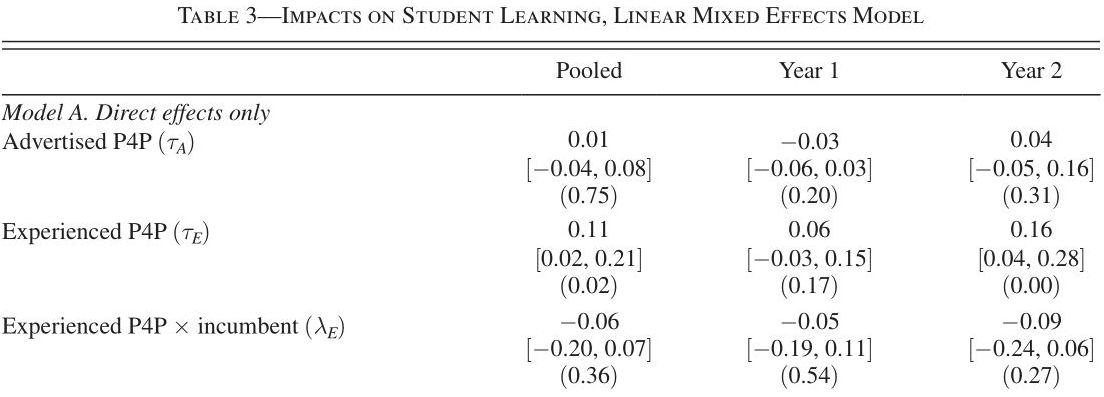
\includegraphics[width = .75\paperwidth]{HK/figure/Leaver_Tab3ModelA.jpg}\\
\vspace{-1ex}{\footnotesize 出所: \citet[][]{Leaver2021}}{\scriptsize $z_{ibksr}=\tau_{A}T^{A}_{qd}+\tau_{E}T^{E}_{s}+\lambda_{I}I_{j}+\lambda_{E}T^{E}_{s}I_{j}+\rho_{br}\bar{z}_{ks,r-1}+\delta_{d}+\phi_{r}+e_{ibksr}$}}
};
\onslide<2->{\node (a1) [rectangle, thick, rounded corners, minimum height = .9cm, minimum width = .75\paperwidth, fill = red, draw=red, fill opacity=.1] at (0cm, .55cm){};}
\onslide<4->{\node (a2) [rectangle, thick, rounded corners, minimum height = .9cm, minimum width = .75\paperwidth, draw=blue, fill = blue, fill opacity=.1, below of = a1, yshift = .0cm]{};}
\end{tikzpicture}
\column{.2\paperwidth}
\begin{tikzpicture}[inner sep=0pt, remember picture]
\node (b0) at (0, 0) {\mpage{.2\paperwidth}{\footnotesize \hfil 現職*FWとの対比\\
\hfil 点推計値\\\hfil [95\%信頼区間]\\\hfil ($p$値)}};
\onslide<3->{\node (b1) at (0, -1.75) {\mpage{.2\paperwidth}{\footnotesize Selection効果: 習熟度にほぼ影響なし}};}
\onslide<5->{\node (b2) at (0, -3) {\mpage{.2\paperwidth}{\footnotesize Contract効果: 習熟度を16\%std高める}};}
\end{tikzpicture}
\begin{tikzpicture}[remember picture, overlay]
\onslide<3->{\draw[red, very thick, ->] (b1.north) .. controls +(-.1, 1.5) and +(-.1, 1.5) .. (a1.north);}
\onslide<5->{\draw[blue, very thick, ->] (b2.south) to [out=-90, in=-90] (a2.south);}
\end{tikzpicture}
\end{columns}
\begin{columns}[T]
\column{.5\paperwidth}
\onslide<6->{\hfill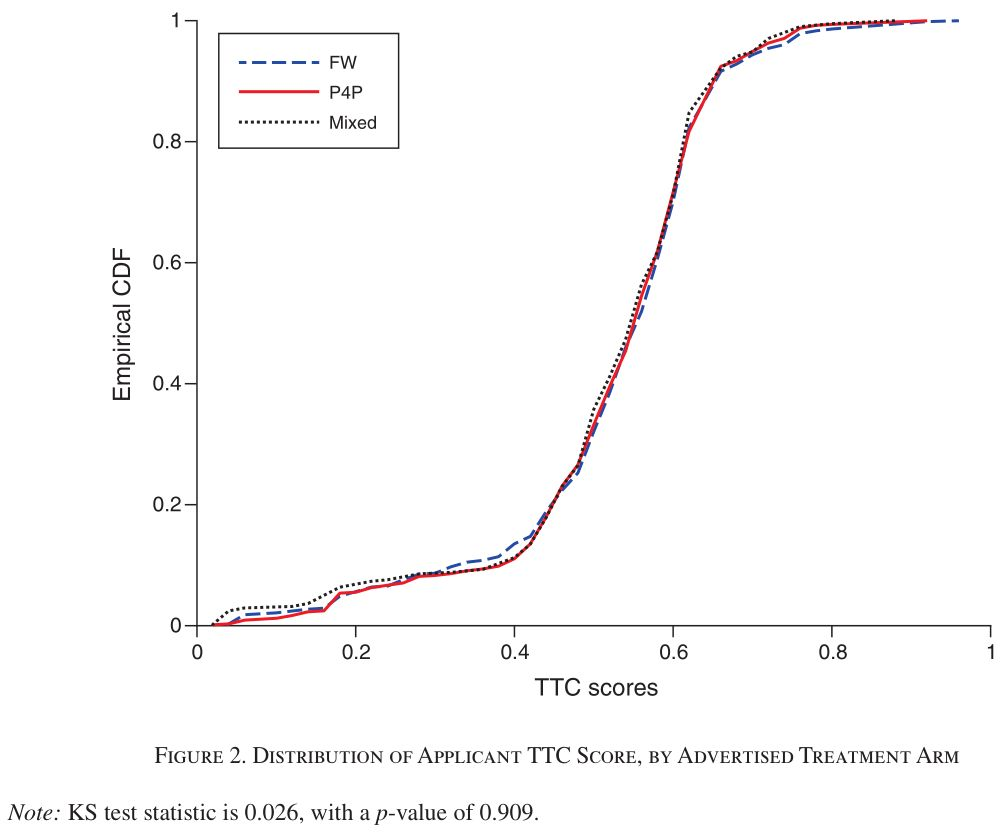
\includegraphics[width = .275\paperwidth]{HK/figure/Leaver_Fig2.jpg}}
\column{.5\paperwidth}
\onslide<7->{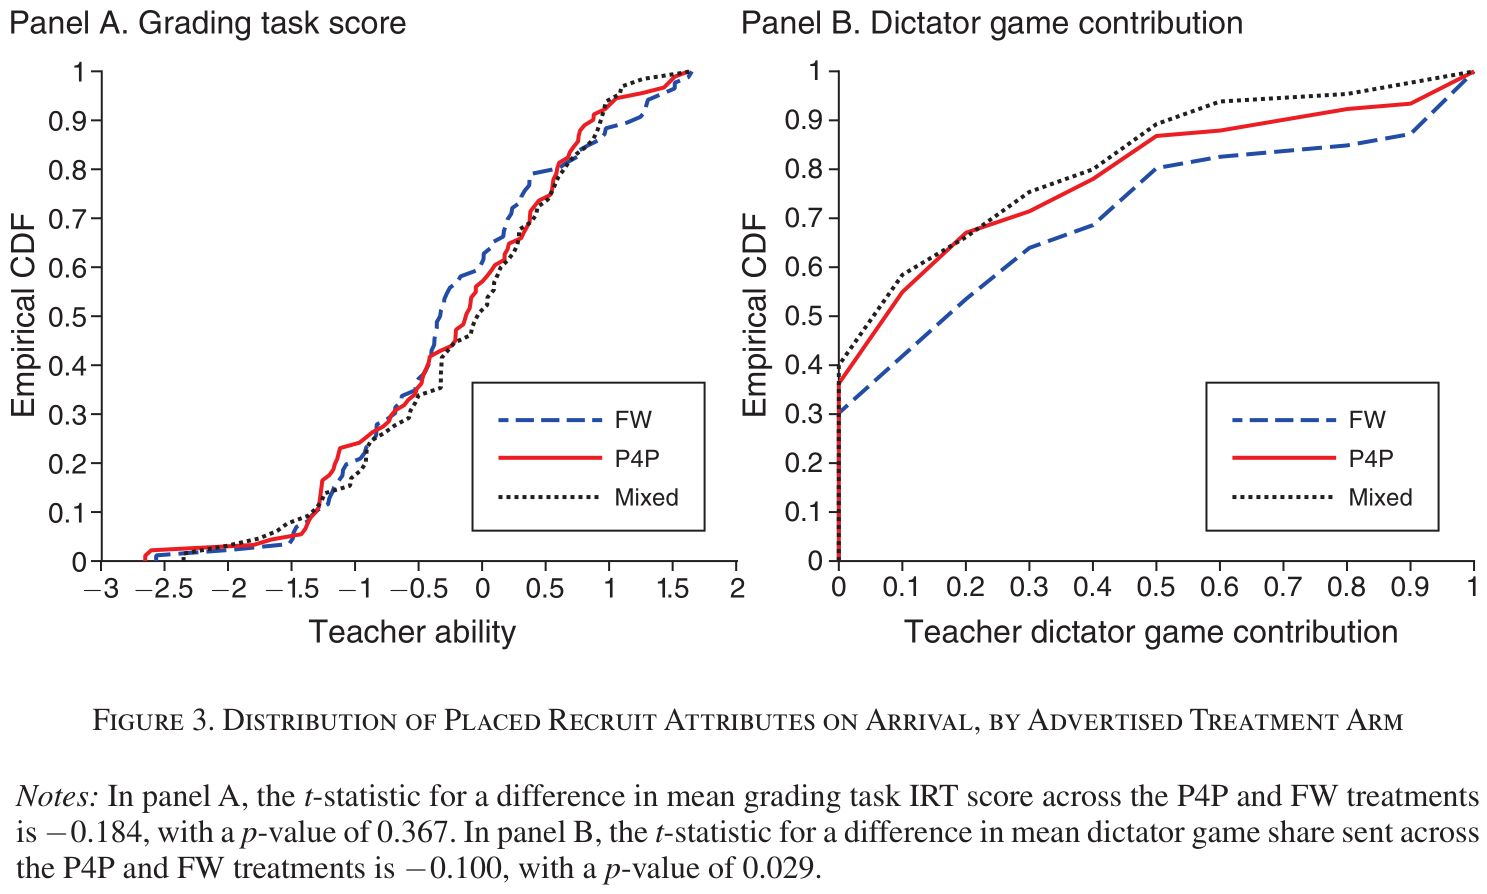
\includegraphics[width = .5\paperwidth]{HK/figure/Leaver_Fig3.jpg}}
\end{columns}
\end{frame}

\begin{frame}[t, label=LeaverResultsSelection]{}
\begin{columns}[T]
\column{.75\paperwidth}
\begin{tikzpicture}[inner sep=0pt, remember picture]
\node at (0, 0) {
\mpage{.75\paperwidth}{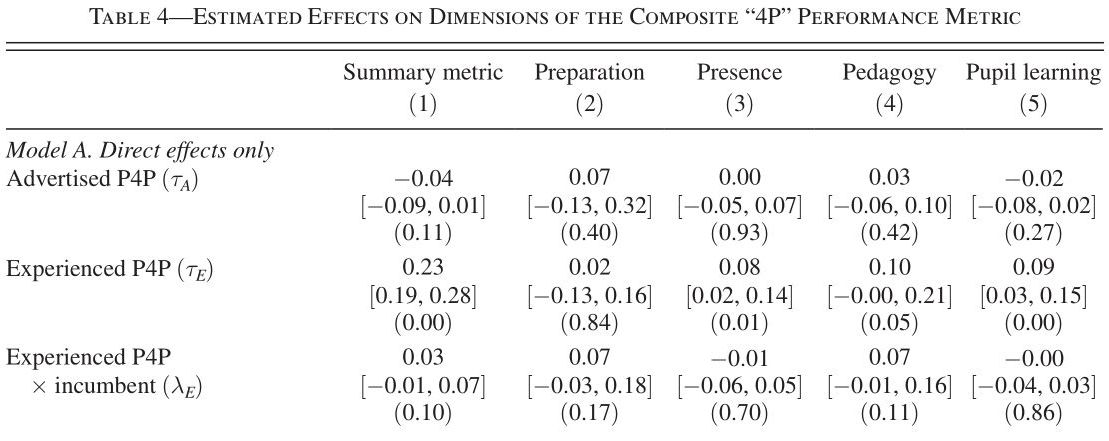
\includegraphics[width = .75\paperwidth]{HK/figure/Leaver_Tab4ModelA.jpg}\\
\vspace{-1ex}{\footnotesize 出所: \citet{Leaver2021}}}
};
\onslide<2->{\node (a1) [rectangle, thick, rounded corners, minimum height = .9cm, minimum width = .75\paperwidth, fill = red, draw=red, fill opacity=.1] at (0cm, .36cm){};}
\onslide<4->{\node (a2) [rectangle, thick, rounded corners, minimum height = .9cm, minimum width = .75\paperwidth, draw=blue, fill = blue, fill opacity=.1, below of = a1, yshift = .0cm]{};}
\end{tikzpicture}
\column{.2\paperwidth}
\begin{tikzpicture}[inner sep=0pt, remember picture]
\node (b0) at (0, 0) {\mpage{.2\paperwidth}{\footnotesize \hfil 現職*FWとの対比\\\hfil 点推計値\\\hfil [95\%信頼区間]\\\hfil ($p$値)}};
\onslide<3->{\node (b1) at (0, -1.75) {\mpage{.2\paperwidth}{\footnotesize Selection効果: 4P'sにほぼ影響なし}};}
\onslide<5->{\node (b2) at (0, -4) {\mpage{.2\paperwidth}{\footnotesize Contract効果:\\ Presenceを8\%、\\ pedagogy点数を10\%高める}};}
\end{tikzpicture}
\begin{tikzpicture}[remember picture, overlay]
\onslide<3->{\draw[red, very thick, ->] (b1.north) .. controls +(-.1, 1.5) and +(-.1, 1.5) .. (a1.north);}
\onslide<5->{\draw[blue, very thick, ->] (b2.south) to [out=-90, in=-90] (a2.south);}
\end{tikzpicture}
\end{columns}
\end{frame}

\begin{frame}[t]{}
\begin{itemize}
\vspace{1.0ex}\setlength{\itemsep}{1.0ex}\setlength{\baselineskip}{12pt}
\onslide<1->{\item	selection効果: }
\begin{itemize}
\vspace{1.0ex}\setlength{\itemsep}{1.0ex}\setlength{\baselineskip}{12pt}
\onslide<2->{\item	投入: Preparation, predagogy, presenceに効果なし}
\onslide<3->{\item	結果: TTC点数はなし(Fig 2)、独裁者ゲームでの渡す額が少ない (Fig 3)、習熟度にほぼ影響なし(Tab 3, Model A, Row1、4\%だがp値=.31)}
\end{itemize}
\onslide<1->{\item	contract効果: }
\begin{itemize}
\vspace{1.0ex}\setlength{\itemsep}{1.0ex}\setlength{\baselineskip}{12pt}
\onslide<4->{\item	投入: Pedagogy, presenceに効果あり}
\onslide<5->{\item	結果: 習熟度に16\%std(Fig 3, Model A, Row 2)}
\onslide<6->{\item	retention: FWと同じ}
\end{itemize}
\end{itemize}
\vspace{2ex}
\onslide<7->{16\%+4\%=20\%の効果ありと結論しているが、4\%のp値は.31}\\~\\
\onslide<8->{
自己中な先生が多く来たけど成果は出ている。P4Pの懸念は発見できず。\\~\\
P4Pはルワンダの既存制度で実施可能: 年1回の実力テスト、出勤チェック、教授法評価、授業計画など
}
\end{frame}

\begin{frame}[t]{まとめ}
\begin{itemize}
\vspace{1.0ex}\setlength{\itemsep}{2.0ex}\setlength{\baselineskip}{12pt}
\item	人的資本: 知的能力(知識、技能)と物的能力(健康)
\pause
\item	教育=技能(人的資本)投資、生涯効用最大化目的に最適な就学時間
\pause
\item	微分を使った最適な就学時間: 就学時間の限界便益=就学時間の限界費用、信用制約の影響
\pause
\item	Inclusive growth: 需要が伸びる技能の取得、アメリカの高卒中流階級
\pause
\item	Directed technical change: 豊富な生産要素を多く使う技術への変化、skill biased technical changeによる大卒以上とそれ以外の格差拡大、近年では平均的大卒も伸び悩む
\pause
\item	途上国: それ以前の段階、どうすれば中学校などで学生の技能が伸びるか実験
\end{itemize}
\end{frame}


\begin{frame}[allowframebreaks]{References}
\scriptsize
\setlength{\baselineskip}{8pt}
\bibliographystyle{aer}
\bibliography{c:/seiro/settings/TeX/seiro}
\end{frame}

\setbeamercovered{invisible}
\begin{frame}[label=LShare]{}
\begin{columns}[T]
\column{.55\textwidth}
\onslide<1->{ 労働分配率(=労働所得/国民所得)\\
 \vspace{-0ex}
 \hfil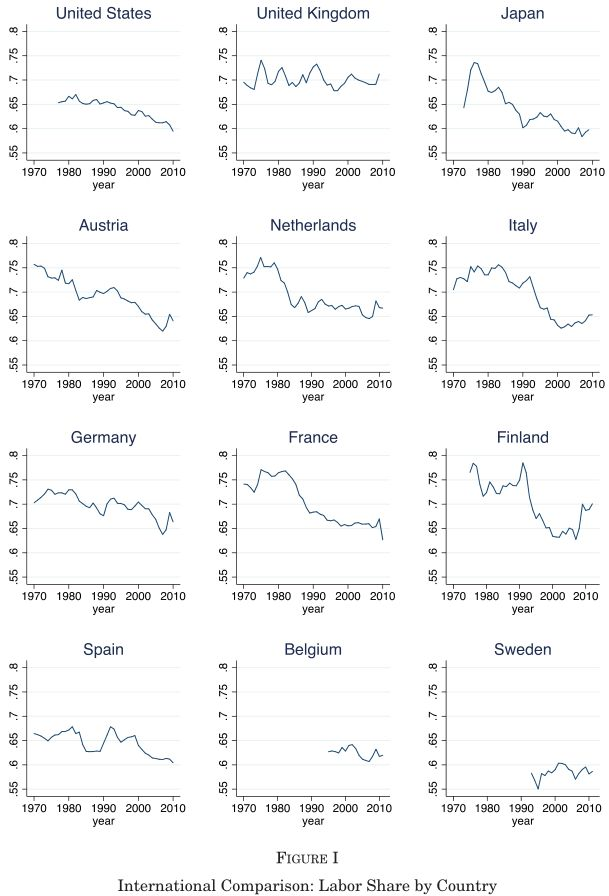
\includegraphics[height = 5cm, width = 7cm]{c:/seiro/docs/external/seishin/lec_slides/2024/HK/figure/ADKPV2021_Fig1small.jpg}\\
 {\footnotesize 出所: \citet[][Figure 1]{ADKPV2020}}
 }
\column{.5\textwidth}
\begin{itemize}
\vspace{1.0ex}\setlength{\itemsep}{1.0ex}\setlength{\baselineskip}{12pt}
\onslide<1->{\item	労働分配率は1980年代からすべての国で低下、日本では-7.143\%低下}
%\onslide<5->{\item	一人あたりGDPが低下していない限り、就業率*労働力率か平均労働所得か(もしくは両方)が低下}
\onslide<5->{\item	1991-2012: 就業率*労働力率は-0.491\%変化(次2枚のスライド)、1人あたりGDPは17.191\%成長}
\onslide<6->{\item	労働分配率の低下の主な背景: 1人あたりGDP成長率(17.191\%)よりも平均労働所得の成長率(10.539\%)が低かったため。就業率や労働力率の影響は小さい。}
\onslide<7->{\item	1人あたりGDPの増分から、労働者よりも多くを企業所有者が得た。所有者と株主が富を増やした。}
\end{itemize}
\end{columns}
\[
\footnotesize
\onslide<2->{\mbox{労働分配率}
=\frac{\mbox{労働所得}}{\mbox{GDP}}
}
%=\frac{\frac{\mbox{労働所得}}{\mbox{人口}}}{\frac{\mbox{GDP}}{\mbox{人口}}}
\onslide<3->{=\frac{\frac{\mbox{労働所得}}{\mbox{労働者数}}\frac{\mbox{労働者数}}{\mbox{労働力}}\frac{\mbox{労働力}}{\mbox{人口}}}{\frac{\mbox{GDP}}{\mbox{人口}}}
}
\onslide<4->{=\frac{\mbox{平均労働所得}\times\mbox{就業率}\times\mbox{労働力率}}{\mbox{1人あたりGDP}}.
}
\]
 \end{frame}

\begin{frame}[label=JapanLShare]{}
日本の労働分配率\\
 \hfil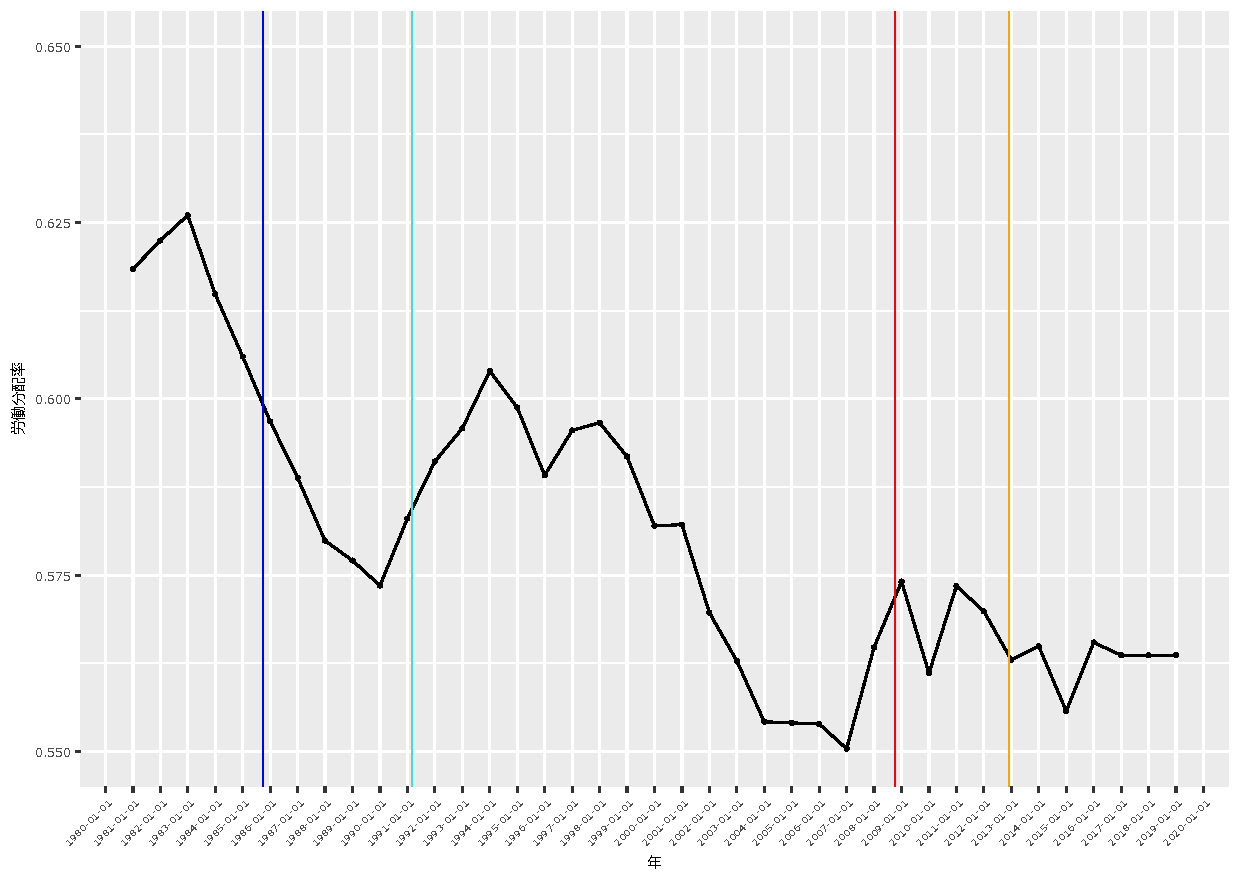
\includegraphics[width = 9.5cm]{c:/seiro/docs/external/seishin/lec_slides/2024/HK/figure/LabourSharesFRED.pdf}\\
 {\footnotesize 出所: \url{https://fred.stlouisfed.org/series/LABSHPJPA156NRUG} University of Groningen and University of California, Davis, Share of Labour Compensation in GDP at Current National Prices for Japan.}
\end{frame}

\begin{frame}[label=JapanLShareGrowthDecomp]{}
微分を使うと以下を示すことができます。$g(x)$は$x$の変化率のことです。
\[
a=\frac{b*c*d}{e} \quad \Rightarrow \quad g(a)=g(b)+g(c)+g(d)-g(e).
\]
\pause
これを労働分配率の分解式に変化率の数字とともに当てはめると以下になります。
\[
\underbrace{0.929-1}_{\mbox{\footnotesize 労働分配率変化率}}=%\frac{\mbox{平均労働所得}\times(\mbox{就業率}\times\mbox{労働力率})\downarrow}{\mbox{一人あたりGDP}\uparrow}
\underbrace{g(\mbox{平均労働所得})}_{\mbox{\footnotesize 平均労働所得変化率}}+\underbrace{(-0.0049083)}_{\mbox{\footnotesize 就業率*労働力率変化率}}-\underbrace{0.1719138}_{\mbox{\footnotesize 1人あたりGDP変化率}}
\]
1991-2012年の平均労働所得成長率=(0.929-1)+(1.1719138-1)-(0.9950917-1)=
0.1053872.
 \end{frame}

 \begin{frame}[label=LForceRates]{}
\begin{columns}[T]
\column{.7\textwidth}
 \onslide<1->{
 労働力率(=労働力人口/人口)\\
 \vspace{-0ex}
 \hfil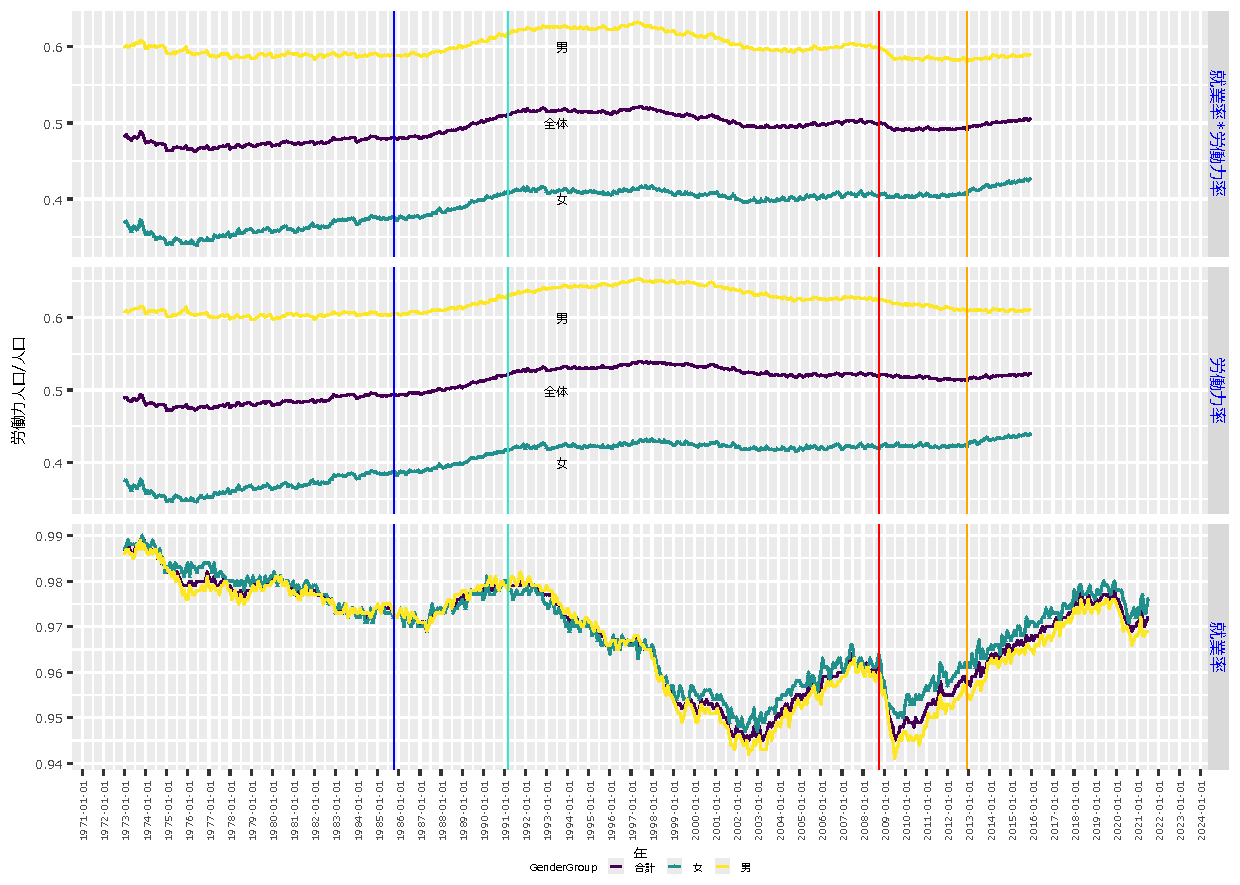
\includegraphics[height = 7cm, width = 10cm]{c:/seiro/docs/external/seishin/lec_slides/2024/HK/figure/LabourForceRates.pdf}
}
\column{.3\textwidth}
\begin{itemize}
\vspace{1.0ex}\setlength{\itemsep}{1.0ex}\setlength{\baselineskip}{12pt}
\onslide<2->{\item	就業率は変化しているが小幅なので、就業率*労働力率はほぼ労働力率で決まる}
\onslide<3->{\item	1997-2012: 労働力率は低下}
\onslide<4->{\item	2013- : 労働力率は上昇}
\onslide<5->{\item	女性の労働力率: 1991年から低下せずに上昇}
\onslide<6->{\item	女性の労働力率: 2013年から急速に上昇}
\end{itemize}
\end{columns}
{\footnotesize 出所: 総務省統計局「労働力統計」長期時系列データ、「人口推計」(政府統計コード=00200524)}
\end{frame}

\begin{frame}[label=LShareJapanByMaritalStatus]{}
\begin{columns}[T]
\column{.7\textwidth}
\onslide<1->{婚姻状態別労働力率\\
\vspace{-0ex}
\hfil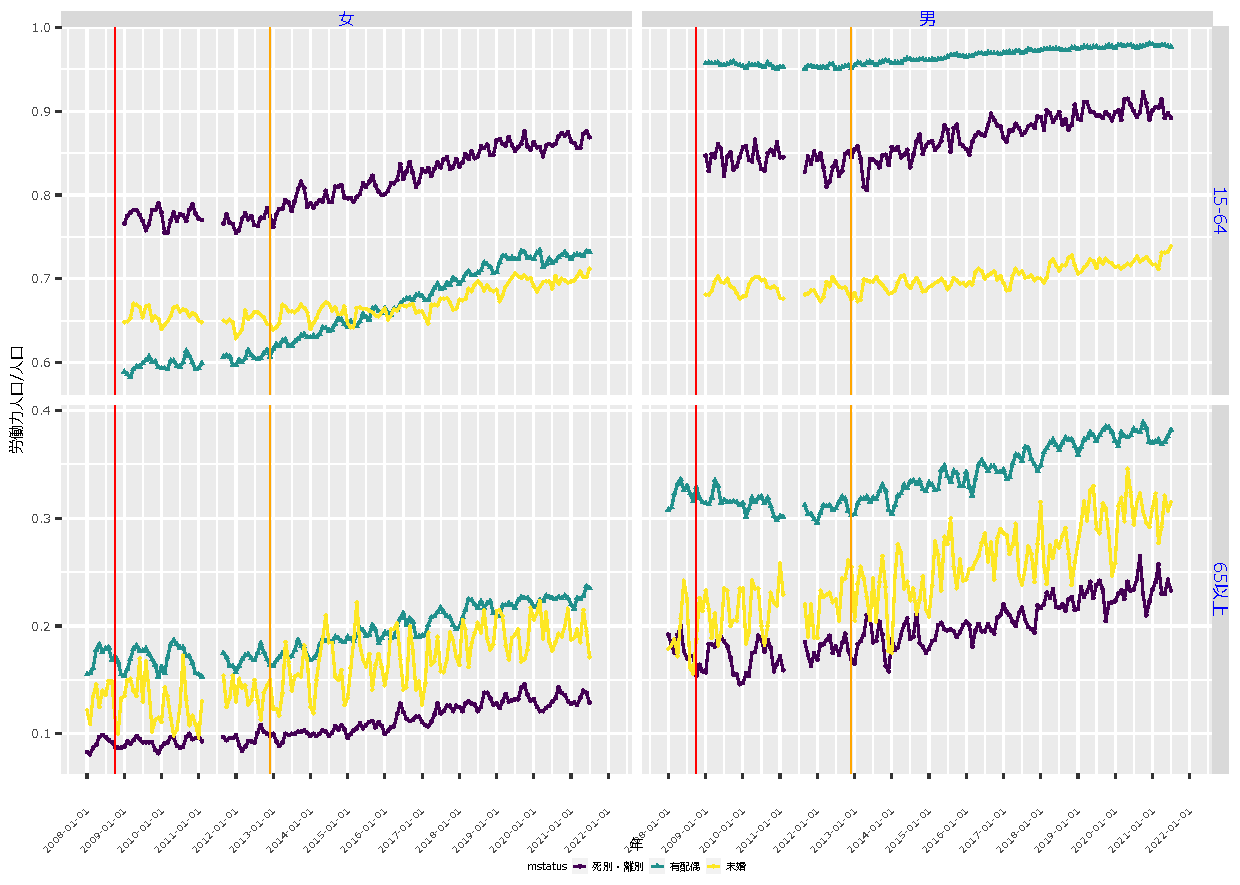
\includegraphics[height = 6cm, width = 10cm]{c:/seiro/docs/external/seishin/lec_slides/2024/HK/figure/LabourForceRatesByMaritalStatus.pdf}\\
{\footnotesize 出所: 総務省統計局「労働力統計」表番号 1-4-5}
}
\column{.3\textwidth}
\begin{itemize}
\vspace{1.0ex}\setlength{\itemsep}{1.0ex}\setlength{\baselineskip}{12pt}
\onslide<2->{\item	女性で労働力率が急速に上昇したグループ: 15-64の有配偶者、死別・離別}
\onslide<3->{\item	未婚女性よりも平均的に年齢が上のグループ$\leftarrow$非正規雇用が多い}
\onslide<4->{\item	労働力率が高まっているが、非正規雇用が増えると平均労働所得が下がるので、労働分配率はどうなるか不明}
\end{itemize}
\onslide<5->{\hfill\hyperlink{Schultz<4>}{\beamergotobutton{Schultz}}}
\end{columns}

 \end{frame}



\end{document}




\begin{frame}{}
\def\trone{3.616335cm}
\def\trtwo{4.590338cm}
\def\trthree{5.793327cm}
DALY of mobidity and injuries, 2010\\
\mpage{5cm}{\mpage{\trone}{\hfil East Asia\\
\hfil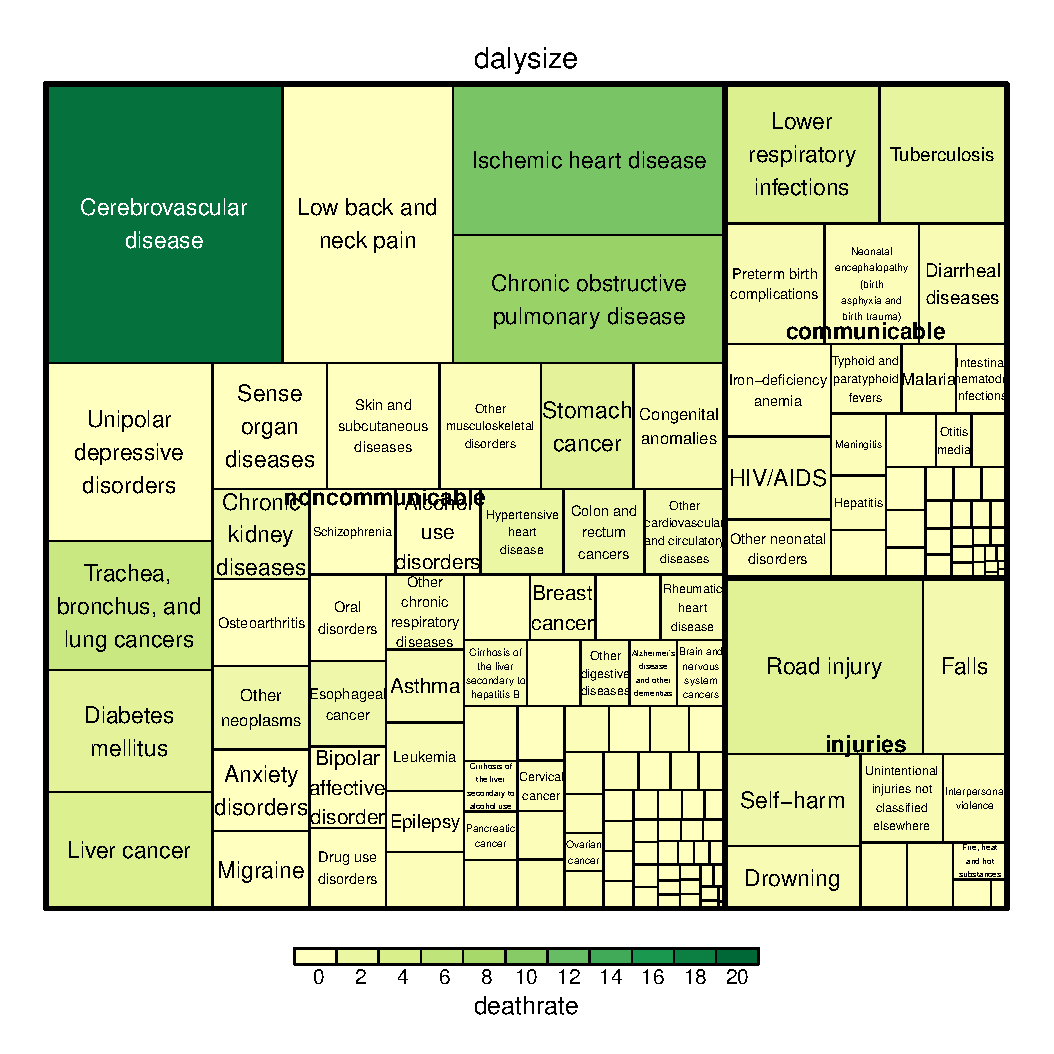
\includegraphics[clip, width = \trone]{c:/seiro/docs/external/seishin/lec_slides/2024/HK/figure/daly_rate_east_asia.eps}}\\
\mpage{\trtwo}{\hfil South Asia\\
\hfil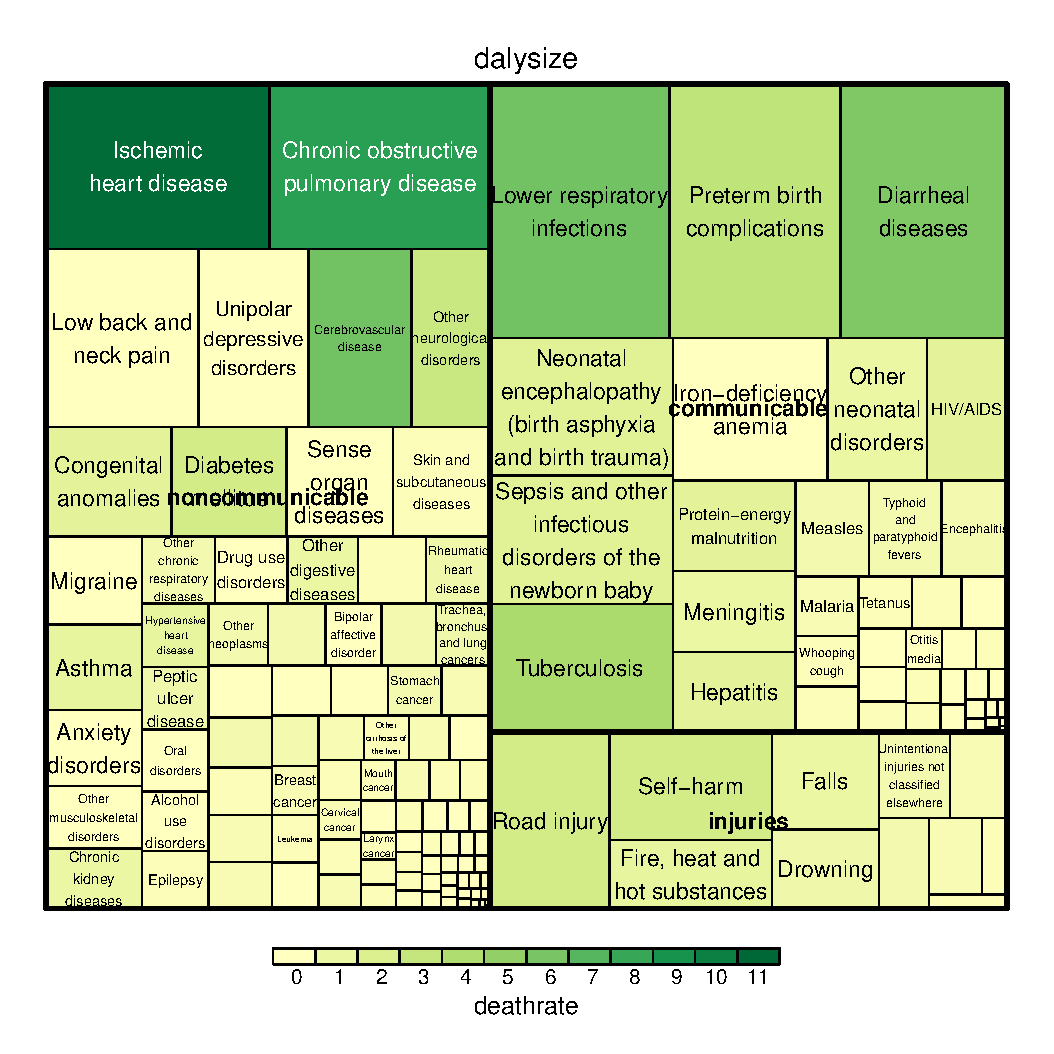
\includegraphics[clip, width = \trtwo]{c:/seiro/docs/external/seishin/lec_slides/2024/HK/figure/daly_rate_south_asia.eps}}
\pause\mpage{\trthree}{\hfil Sub-Saharan Africa\\
\hfil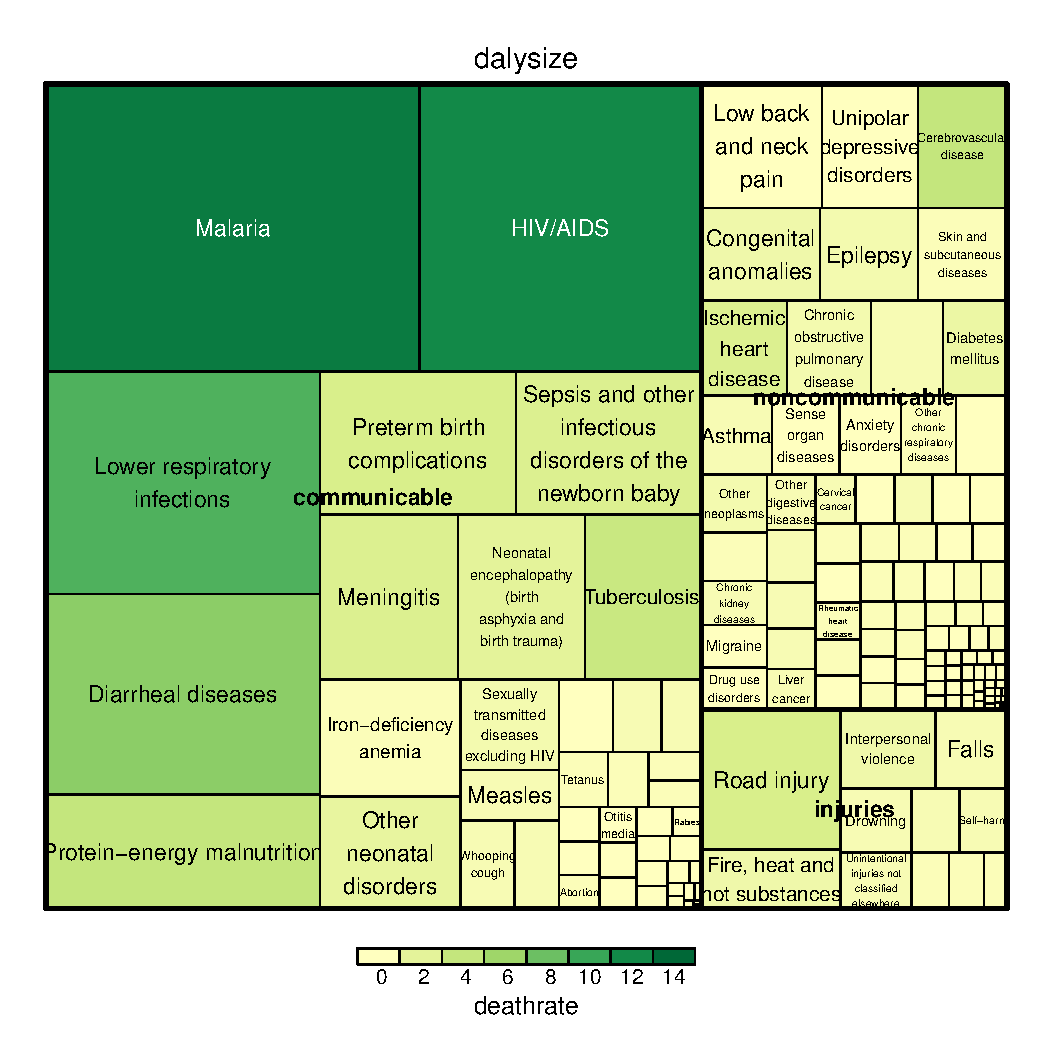
\includegraphics[clip, width = \trthree]{c:/seiro/docs/external/seishin/lec_slides/2024/HK/figure/daly_rate_sub-saharan_africa.eps}}\\
{\footnotesize Global Burden of Diseases, 2010(\url{http://viz.healthmetricsandevaluation.org/gbd-compare/})}}
\end{frame}

\begin{frame}{}
Disability Adjusted Life Years: DALY\\~\\

Shows how much years are lost to sickness and injuries.\\

Sickness A takes away $a$ years of healthy life, sickness $b$ takes away $b$ years, ....count the morbid, and multiply to get national DALY.\\~\\

There are obvious oversimplification and biases, but if we need to get some metric, we need to assume something and compute. It gives a rough idea of what is going on in the world in terms of health.
\end{frame}

\begin{frame}{}
Morbidity has intrinsic disutility. But when using economics, we consider its productive impacts.\\~\\

If health is damaged, the body needs a rest and/or human capital is damaged. The sick cannot work as productively as before if working in the same way. If an adult dies from a disease/an injury, the accumulated skill will be lost. \\~\\

So one should weigh the (marginal) benefits and (marginal) costs of interventions.\\~\\

Given a disease, if we can reduce an average patient (so marginal benefit is fixed), the marginal costs are:
\[
\mbox{health promotion} > \mbox{prevention} > \mbox{treatment}.
\]
\end{frame}

\begin{frame}{}
One seemingly cost effective intervention is deworming.\\
\pause
\hfil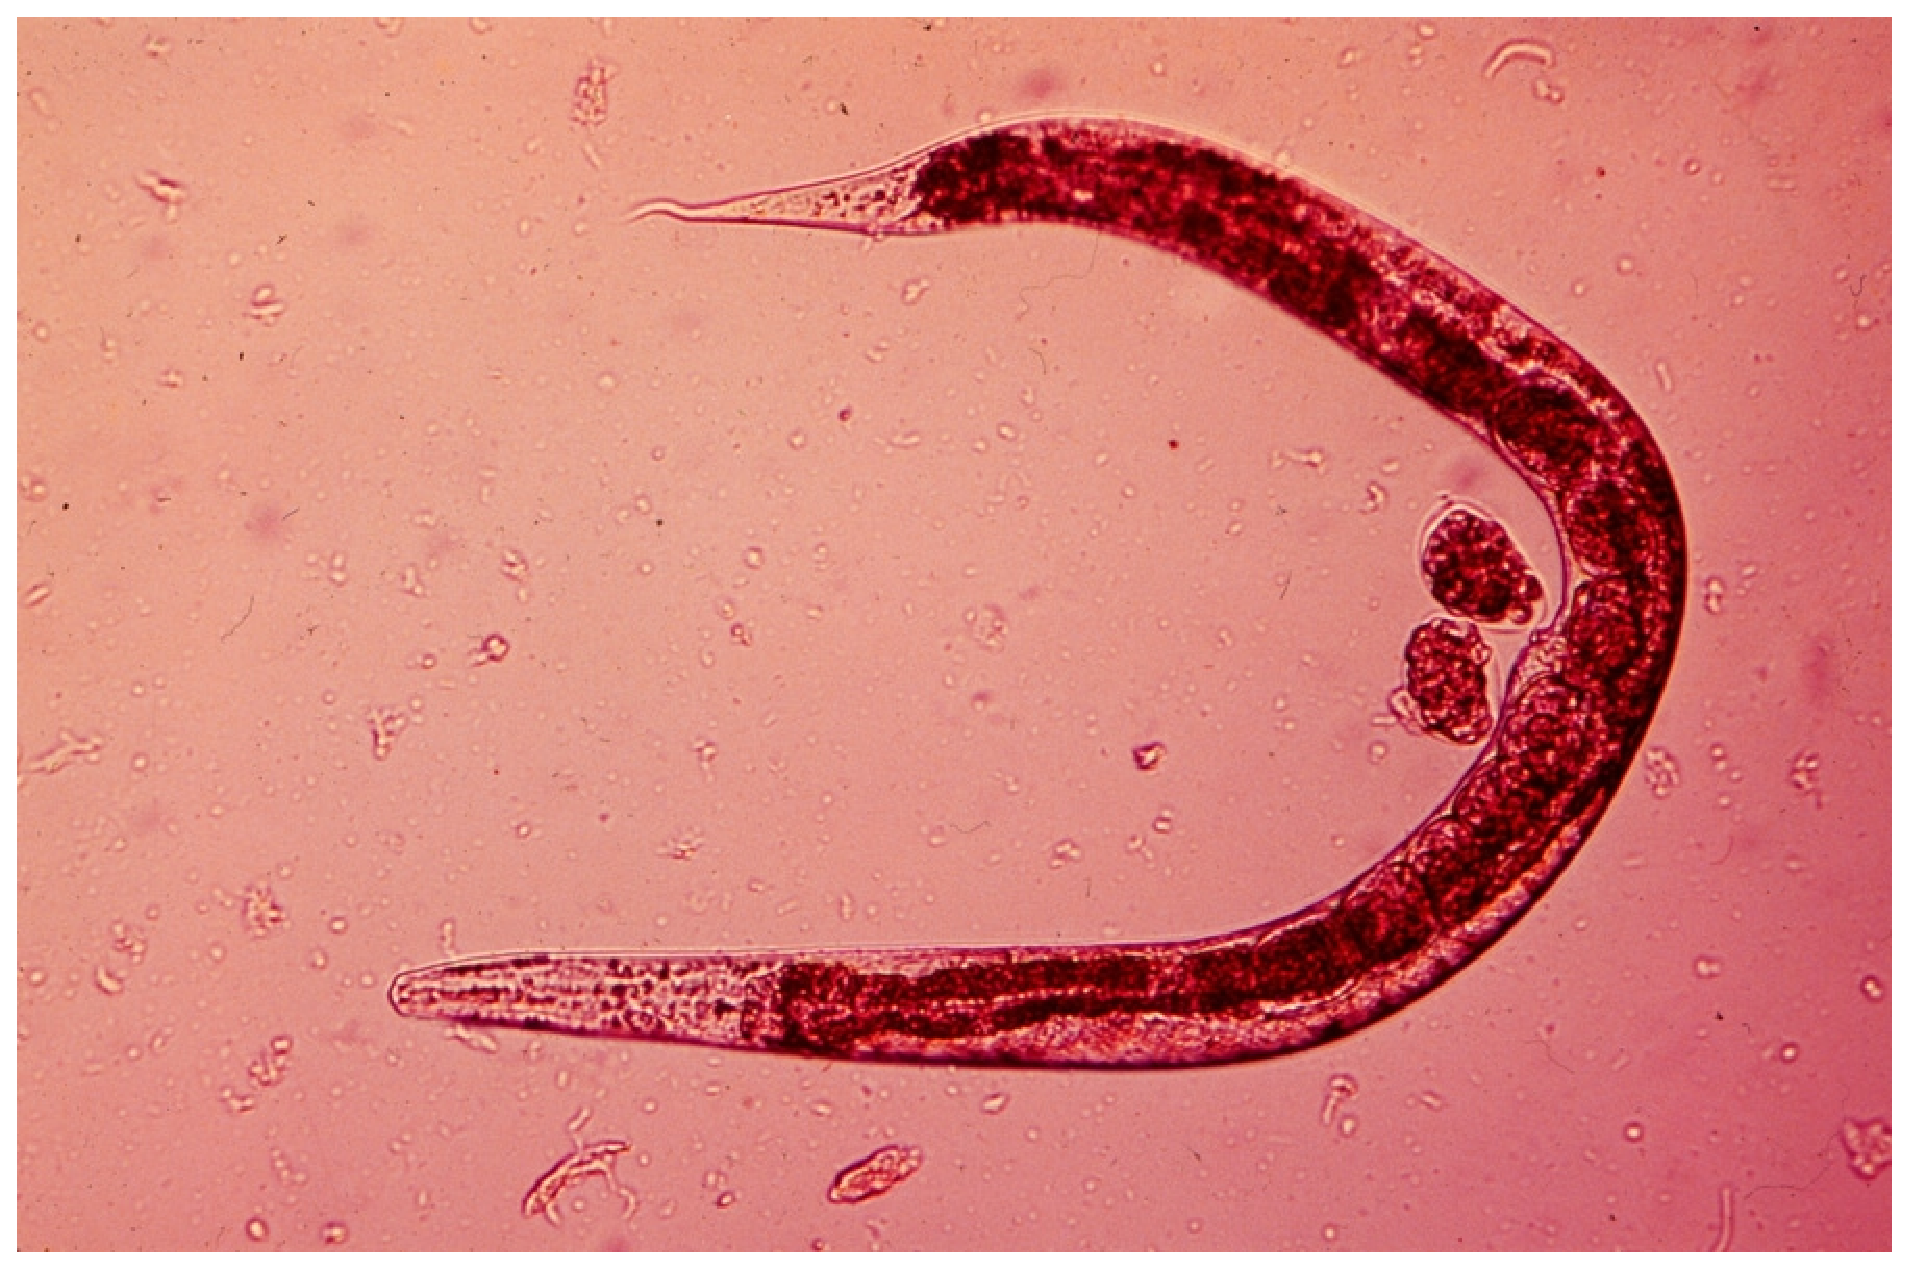
\includegraphics[clip, width = 10cm]{c:/seiro/docs/external/seishin/lec_slides/2024/HK/figure/helminth.eps}
\end{frame}

\begin{frame}{}
Soil transmitted helminth (STH) worms can lead to
\begin{itemize}
\vspace{1.0ex}\setlength{\itemsep}{1.0ex}\setlength{\baselineskip}{12pt}
\item	Iron deficiency anaemia.
\item	Protein energy malnutrition.
\item	Schistosomaiasis: Enlargement of liver and spreen.
\item	Symptom also include underdevelopment of cognitive skills.
\end{itemize}

\vspace{2ex}
Treatment is easy: Take a drug. \\~\\

\pause
But treatment is lengthy, because of relapse (reinfection). \\~\\

\pause
Why reinfected? \\~\\
\pause
Because people around you are infected and not being treated!
\end{frame}

\begin{frame}{}
\citet{MiguelKremer2004} ran an experiment to distribute deworming tablets among students in Western Kenya.\\~\\

\pause
It is not about if drugs are effective. We know that these tablets are effective.\\~\\

\pause
It is about treatment externality.\\~\\

\pause
They randomised the distribution of tablets among schools (unit of intervention is not students, so pretty much all students who agreed to participate got the medication). \\~\\

\pause
For any student $i$ who goes to the control school, the number of students $x_{i}$ in the neighbourhood going to the treated school is random. So regressing the outcomes $y_{i}$ of control school students on $x_{i}$ gives a consistent estimate of treatment extenality. A nice idea.\\~\\
\pause
They used DID.
\end{frame}

\begin{frame}{}
\hfil\includegraphics[clip, width = 10cm]{c:/seiro/docs/external/seishin/lec_slides/2024/HK/figure/hicks_fig1.eps}
\end{frame}

\begin{frame}{}
There was a controvercy between epidemiologists and economists. Epidemiologists undertook a replication study using the same data set. The study was funded by 3ie. \\~\\

\pause
Epidemiologists found:
\begin{itemize}
\vspace{1.0ex}\setlength{\itemsep}{1.0ex}\setlength{\baselineskip}{12pt}
\pause
\item	Errors in estimation code. 
	\begin{dinglist}{43}
	\vspace{1.0ex}\setlength{\itemsep}{1.0ex}\setlength{\baselineskip}{12pt}
\pause
	\item	Original authors acknowledged.
	\end{dinglist}
\pause
\item	After correcting for errors, and some results became statistically zero. They did not use DID, but a logistic regression (a nonlinear regression like probit). The 1st year impact was about 1.2, 2nd year impact was 1.4, and combined 1st and 2nd year impact was 1.8. They wondered why it is not between 1.2 and 1.4
	\begin{dinglist}{43}
	\vspace{1.0ex}\setlength{\itemsep}{1.0ex}\setlength{\baselineskip}{12pt}
\pause
	\item	Original authors disagreed. They stuck with DID.
\pause
	\item	Because logistic regression is nonlinear, combined effect can go outside ``parts''.
	\end{dinglist}
\end{itemize}
\end{frame}

\begin{frame}{}
So epidemiologists might have confused with nonlinearity.\\~\\

\pause
But it seems like the common trend assumption might have not been satisfied. There were 3 groups, and 2 groups reduced school attendance rates but not so for the remaining group. Remaining group was the treated in year 2.\\~\\

\pause
It is good to have replication studies and discuss about the generalisability of findings.\\~\\

\pause
But one must be cautious about the problem of \textit{multiple testing}.
\end{frame}


\begin{frame}[allowframebreaks]{References}
\scriptsize
\setlength{\baselineskip}{8pt}
\bibliographystyle{aer}
\bibliography{c:/seiro/settings/TeX/seiro}
\end{frame}


\begin{frame}{Extension: ECD}
We assumed that child learning capacity is homogenous $h(L-l)$ is same for everyone with same $l$. \\~\\

This is hardly true. Let us rewrite:
\[
h=h(L-l)^{1+a}, \quad a>0.
\]
Let us assume that parents can `buy' an extra boost to human capital $a$ at price $p_{a}$:
\[
A+w_{1}l=c_{1}+c_{p,1}+p_{a}a+s.
\]
\end{frame}

\begin{frame}{}
Then the problem is:
\[
\begin{aligned}
\max_{\{s, a, c_{1}, l\}}
& \;\;\; u_{p}(A+w_{1}l-c_{1}-p_{a}a-s)\\
& \;\;\;\hspace{1em}+\delta \{u(c_{1})+\beta u(h^{1+a}w_{2}+s)\}\\
\st & \;\;\; s\geqslant 0, \ a\geqslant 0
\end{aligned}
\]
\[
\begin{aligned}
\mathcal L&=u_{p}(A+w_{1}l-c_{1}-p_{a}a-s)\\
&\hspace{2em}+\delta \{u(c_{1})+\beta u(h^{1+a}w_{2}+s)\}\\
&\hspace{2em}+\lambda_{s}[s-0]+\lambda_{a}[a-0].
\end{aligned}
\]
FOCs
\[
\begin{aligned}
\mathcal L_{s}&=-u'_{p}+\delta\beta u'_{2}+\lambda_{s}^{*}\leqslant 0,\; & \lambda_{s}^{*}&\geqslant 0, 
\; & s^{*}&\geqslant 0, \; & s^{*}\mathcal L_{s}^{*}&= 0,\\
\mathcal L_{a}&=-u'_{p}p_{a}+\delta\beta u'_{2}(1+a)h^{a}w_{2}= 0,\\
\mathcal L_{c_{1}}&=-u'_{p}+\delta u'_{1}=0,\\
\mathcal L_{l}&=u'_{p}w_{1}-\delta\beta u'_{2}(1+a)h^{a}w_{2}h'= 0.
\end{aligned}
\]
\end{frame}
\begin{frame}{}
If $a^{*}>0$
\[
-u'_{p}p_{a}+\delta\beta u'_{2}(1+a)h^{a}w_{2}= 0, \quad
u'_{p}w_{1}-\delta\beta u'_{2}(1+a)h^{a}w_{2}h'= 0.
\]
Replace $u'_{p}$ with $\delta u'_{1}$:
\[
\begin{aligned}
-\delta u'_{1}+\delta\beta u'_{2}+\lambda&\leqslant 0, \quad s\geqslant 0,\\
-\delta u'_{1}p_{a}+\delta\beta u'_{2}(1+a)h^{a}w_{2}&=0,\\
\delta u'_{1}w_{1}-\delta\beta u'_{2}(1+a)h^{a}w_{2}h'&= 0.
\end{aligned}
\]
Latter 2 give
\[
\frac{w_{1}}{p_{a}}=h'.
\]
LHS is relative costs of invest in $a$
\end{frame}
\begin{frame}{}
\[
\begin{aligned}
hw_{2}&=p_{a},\\
(1+a)h'w_{2}&=w_{1}.
\end{aligned}
\]
First of these indicate that parents will buy $a$ to equate marginal gain $hw_{2}$ 	with its marginal cost $p_{a}$. The human capital investment will be done according to equating marginal gain $(1+a)h'w_{2}$ with marginal cost $w_{1}$. 
\end{frame}
\begin{frame}{}
Suppose the household is liquidity contsrained.
\[
-u'_{p}+\delta\beta u'_{2}+\lambda_{s}^{*}<0.
\]
\end{frame}
\begin{frame}{}
\[
\begin{aligned}
s&: -u'_{p}+\delta\gamma\beta u'_{2}=0,\\
a&: -u'_{p}p_{a}+\delta\beta u'_{2}hw_{2}=0,\\
c_{1}&: -u'_{p}+\delta u'_{2}=0,\\
l&: u'_{p}w_{1}-\delta\gamma\beta u'_{2}w_{2}ah'=0.
\end{aligned}
\]
\[
\begin{aligned}
\mathcal L_{s}&=-u'_{p}+\delta\gamma\beta u'_{2}\leqslant 0,\; & \lambda_{s}^{*}&\geqslant 0, 
\; & s^{*}&\geqslant 0, \; & s^{*}\mathcal L_{s}^{*}&= 0,\\
\mathcal L_{a}&=-u'_{p}+\delta\beta u'_{2}hw_{2}\leqslant 0,\; & \lambda_{a}^{*}&\geqslant 0, 
\; & a^{*}&\geqslant 0, \; & a^{*}\mathcal L_{a}^{*}&= 0,\\
\mathcal L_{c_{1}}&=-u'_{p}+\delta u'_{2}=0,\\
\mathcal L_{l}&=u'_{p}w_{1}-\delta\gamma\beta u'_{2}w_{2}ah'\leqslant 0,\; & \lambda_{l}^{*}&\geqslant 0, 
\; & l^{*}&\geqslant 0, \; & l^{*}\mathcal L_{l}^{*}&= 0.
\end{aligned}
\]
\end{frame}
